\documentclass[a4paper,12pt,notitlepage]{book}
\usepackage[english]{babel}
\usepackage{amsmath, amssymb}
\usepackage{amsthm}
\usepackage{amstext}
\usepackage{array}
\usepackage{graphicx,color,psfrag,pgfplots}
\usepackage[bf,small]{caption}
\usepackage{subfig}
\usepackage{bbm}
\usepackage{wrapfig}
\usepackage{natbib}
\usepackage{listings} % pacchetto per scrivere codice
\usepackage{color}
\usepackage{booktabs}
\usepackage{enumitem}
\usepackage{textcomp}
\usepackage{mathtools}

\usetikzlibrary{patterns,calc,decorations.markings,positioning}

%%%%%%%%%%%%%%PER IL BOX
\usepackage{tikz}
\usetikzlibrary{shapes,positioning,arrows,calc,shadows}
\tikzstyle{abstractbox} = [draw=black, fill=white, rectangle, 
  inner sep=11pt, style=rounded corners] %drop%shadow={fill=gray,opacity=0.8}]
  \tikzstyle{abstracttitle}=[fill=white]  
  \newcommand{\mybox}[3][fill=white]{
    \begin{center}
      \begin{tikzpicture}
        \node [abstractbox, #1] (box)
        {\begin{minipage}{0.95\linewidth}
%           \setlength{\parindent}{2mm}
           \normalsize #2
          \end{minipage}};
        \node[abstracttitle, right=11pt] at (box.north west) {#3};
      \end{tikzpicture}
    \end{center}
  }
%%%%%%%%FINE PER IL BOX


\theoremstyle{plain}
\newtheorem{Teorema}{Theorem}[chapter]

\theoremstyle{definition}
\newtheorem{Definizione}{Definition}[chapter]

\theoremstyle{remark}
\newtheorem{Osservazione}{Observation}[chapter]

\graphicspath{{img/}}

%Comandi personali
\newcommand{\vect}[1]{\mathbf{#1}}
\newcommand{\classe}[1]{\emph{#1}}
\newcommand{\referenza}[1]{[\ref{#1}]}
\newcommand{\referenzaeq}[1]{(\ref{#1})}
\newcommand{\figref}[1]{Fig.\ref{#1}}
\newcommand{\nsp}[1]{\foreach \n in {1,...,#1}{\!}}
\newcommand{\psp}[1]{\foreach \n in {1,...,#1}{\,}}	

\begin{document}

\begin{titlepage}
\begin{center}
    { \scshape 
    Laurea magistrale\\
    in ingegneria matematica\\
    }
\end{center}
\vspace{1.2cm}
\begin{flushleft}
		\Large
		Elaborato di Tesi ...
		\vspace{1.5cm}
\end{flushleft}
\begin{figure}[h]
		\centering
		
\includegraphics[width=0.25\textwidth]{Varie/logo-polimi}
		\vspace{1cm}
\end{figure}
\begin{center}
{ \bfseries  {\Large Titolo progetto di tesi ...}\\
\vspace{0.2cm} }
\end{center}
\vspace{0.4cm}
\begin{flushright}
		\Large
		Progetto svolto da:\\
		Andrea Bortolossi\\
		Matr. 783023\\
		\vspace{1.5cm}
\end{flushright}
\begin{center}
Anno Accademico 2013--2014
\end{center}

\end{titlepage}
\clearpage
\tableofcontents
\chapter*{Estratto della tesi}
\addcontentsline{toc}{chapter}{Estratto della tesi}

%Nel 1947 John Bardeen, William Shockley e Walter Brattain inventarono il transistore bipolare dando inizio ad una crescita esponenziale delle industrie di dispositivi a semiconduttore. Prima di raggiungere le funzionalit\`a dei dispositivi moderni alcuni passi fondamentali sono stati fatti: nel 1958 venne prodotto il primo circuito integrato (IC), seguito dall'introduzione del MOSFET (1960) e dal CMOS (1963). Queste prime scoperte portarono all'invenzione del primo microprocessore (1971): da allora un incessante sviluppo ed una continua opera di miniaturizzazione di tali dispositivi, hanno portato le industrie di microelettronica alla soglia della VLSI era (Very-Large-Scale-Integration). 
%
%Negli ultimi trenta anni questo processo ha garantito performance superiori e riduzione dei costi della produzione dei moderni computer, unit\`a wireless e sistemi di comunicazione, influenzando drasticamente lo stile di vita odierno.
%Gli investimenti spesi nello sviluppo delle tecnologie VLSI, costituitiscono ancora oggi una forza trainante nello sviluppo di dispositivi ad alta densit\`a di integrazione e superiore velocit\`a di risposta.
%
%Grandi sforzi sono stati spesi al fine di comprendere al meglio le dinamiche fisiche che governano il funzionamento dei moderni dispositivi portando ad un sempre pi\`u crescente utilizzo di solutori numerici commerciali.
%Tuttavia affidandosi ad un software esterno risulta ovviamente impossibile avere un pieno controllo delle funzionalit\`a rese disponibili dalla software house. In un ambiente in cos\`i rapida evoluzione tale limitazione pu\`o risultare vincolante e dunque lo sviluppo di un solutore personale \`e auspicabile.
%
%Il progetto FEMOS (\textit{Finite Element Method Oriented Solver}) nasce al fine di sopperire a tale richiesta. Si tratta di un solutore \textit{homemade} in grado di predire il funzionamento dei pi\`u moderni dispositivi, tenendo conto delle interazioni fra i diversi fenomeni caratterizzanti. Il codice \`e scritto in C++ ed \`e costituito da librerie dinamiche orientate alla risoluzione delle dinamiche elettriche, chimiche, meccaniche e termiche utilizzando il metodo agli elementi finiti (FEM). All'interno di questo framework l'obiettivo della tesi \`e di implementare gli strumenti matematici volti alla modellizzazione e simulazione del comportamento elettrico dei dispositivi a semiconduttore. Il lavoro \`e stato svolto nel corso di un'esperienza lavorativa presso Micron Technology (una delle compagnie leader fra le industrie di semiconduttori) ed \`e costituito dalle seguenti librerie:
%
%\begin{itemize}[leftmargin=3.7cm]
%\item[\textit{Semiconductor}] l'oggetto principale di questa libreria \`e la classe \texttt{Semi-} \texttt{conductor}, nella quale sono implementate le relazioni fondamentali fra le quantit\`a caratteristiche dei materiali a semiconduttore.
%
%\item[\textit{NLPsolver}] questa libreria raccoglie le funzioni utili alla gestione del metodo di Newton applicato all'equazione di Poisson.
%
%\item[\textit{DD\_semiconductor}]  in questa libreria sono incluse le funzioni adibite alla gestione della risoluzione dell'equazione di continuit\`a e i metodi volti alla valutazione della corrente ai contatti e all'interno del dispositivo.
%
%\item[\textit{ModelsManage}] l'oggetto principale di questa libreria \`e la classe \texttt{Models-} \texttt{Manage}, il cui compito risiede nel mettere in comunicazione le variabili interne del codice con i modelli (di mobilit\`a e R/G) caricati dall'utente.
%
%\item[\textit{ImplementedModels}] questa libreria raccoglie tutti i modelli di mobilit	\`a e R/G ed \`e stata scritta in modo tale che sia possibile aggiungere nuovi modelli senza mutare altre parti del codice.
%\end{itemize}

Lo sviluppo tecnologico nell'industria dei semiconduttori \`e in rapidissima crescita in questi ultimi anni e in particolare non solo secondo il tradizionale \textit{shrinking tecnologico}, ma grazie anche all'utilizzo di nuovi principi fisici complementari o alternativi alla fisica dei semiconduttori.
In particolare, l'utilizzo di nuovi materiali richiede capacit\`a di sviluppo e comprensione decisamente superiori rispetto al passato. Proprio per rispondere a queste esigenze in Micron Technology (una delle compagnie leader fra le industrie di semiconduttori) \`e nato il progetto FEMOS (\textit{Finite Element Method Oriented Solver}). FEMOS \`e un codice numerico modulare in grado di affrontare problematiche di diversa natura fisico-chimica,  di trasporto termico ed elettronico in mezzi anisotropi e di meccanica dei continui, applicate ai pi\`u moderni dispositivi di memoria (a cambiamento di fase, a movimento ionico).
A completamento di questo progetto si \`e resa necessaria la possibilit\`a di simulare i materiali a semiconduttore: questo lavoro di tesi si inserisce proprio in questo contesto. 
In particolare ci siamo occupati della trattazione dell'approccio Drift-Diffusion \cite{Jackson:ElettroClassica} per i semiconduttori la cui risoluzione si \`e basata sull'algoritmo della mappa di Gummel \cite{GummelMap}. La discretizzazione delle equazioni \`e stata realizzata secondo il metodo di Galerkin agli elementi finiti (FEM) ed in particolare per il problema di Poisson si \`e scelta una formulazione agli spostamenti, mentre per l'equazione di continuit\`a ci si \`e affidati allo schema numerico EAFE presentato in \cite{Zikatanov:EAFE1}. Il problema non lineare di Poisson \`e stato affrontato con il metodo di Newton. 

La parte pi\`u originale del lavoro \`e costituita dalle tecniche sviluppate al fine di calcolare la corrente ai contatti e all'interno dei dispositivi. Nel primo caso abbiamo esteso il metodo dei residui  presentato in \cite{ContactCurrentRM} ad un framework 3D. Per il secondo abbiamo proposto due schemi innovativi volti all'estensione al caso 3D della formula di Scharfetter-Gummel \cite{Gummel:SignAnalys}.

Sono stati condotti test di simulazione su vari dispositivi a semiconduttore (diodo, n-MOSFET/p-MOSFET) ed i risultati ottenuti sono stati confrontati con un solutore commerciale ottenendo un ottimo accordo.
\vspace{1cm}

L'elaborato \`e organizzato nel seguente modo:
\begin{itemize}[leftmargin=2.5cm]
\item[\bf Capitolo 1]  richiamiamo brevemente le propriet\`a fisiche dei semiconduttori ed enunciamo le principali relazioni che intercorrono fra le grandezze fondamentali (potenziale elettrostatico, campo elettrico, densit\`a di portatori e di corrente). Presentiamo il modello Drift-Diffusion e alcuni dei principali modelli di mobilit\`a dei portatori e dei fenomeni di R/G.

\item[\bf Capitolo 2] questo capitolo \`e diviso in due sezioni. Nella prima ci occupiamo di introdurre le geometrie considerate durante le simulazioni e le relative notazioni. Nella seconda parte illustriamo gli algoritmi usati al fine di trattare il modello esposto nel primo capitolo (Gummel map).

\item[\bf Capitolo 3] la buona posizione delle equazioni trattate e i metodi utilizzati per discretizzarle sono approfonditi in questo capitolo. Particolare attenzione poniamo su alcune interessanti difficolt\`a numeriche.

\item[\bf Capitolo 4] questo capitolo contiene i risultati ottenuti. La validazione dei tests \`e stata condotta su dispositivi a semiconduttore tipici (diodo, n-MOSFET/p-MOSFET) confrontando le soluzioni con un software commerciale. La parte finale del capitolo riguarda l'estensione del \textit{metodo dei residui} al caso 3D per il calcolo della corrente ai contatti \cite{ContactCurrentRM}.

\item[\bf Capitolo 5] in questo capitolo vengono trattate alcune tecniche che permettono la ricostruzione delle densit\`a di corrente all'interno dei dispositivi. Proponiamo due schemi innovativi al fine di  estendere la formula Scharfetter-Gummel \cite{Gummel:SignAnalys} al caso 3D. Infine confrontiamo i risulati con il simulatore commerciale.
\end{itemize}


\chapter*{Introduction}
\addcontentsline{toc}{chapter}{Introduction}

%In 1947 John Bardeen, William Shockley and Walter Brattain (three scientists of Bell Telephone Labs) invented the bipolar transistor and since that crucial point there has been a continously increasing growth of the semiconductor industry never known before, with a serious impact on the way people work and live today. 
%
%Before reaching the functionality and the miniaturization of nowdays devices, some fundamental steps have been made.
%In 1958 the first intagrated circuit (IC) was produced, followed by the introduction of the first MOSFET(1960) and CMOS(1963). Into these inventions the first micro-processor (1971) sank his roots  and since that time until present, an ever-increasing progress has continued, according to the indication of \textit{Moore's Law} (formulated by Gordon Moore in 1965).
%
%These events led microelectronic industry at the doors of the VLSI era (Very-Large-Scale-Integration). Indeed in the last thirty years the benefits of miniaturization have been the key in the evolutionary progress leading to today's computers, wireless units, and comunication systems that offer superior performance, dramatically reduced cost per function, and much reduced physical size.
%
%The large worldwide investment in VLSI technology constitutes a formidable driving force that guarantees the continued progress in IC integration density and speed, for as long as physical principles will allow.
%
%From this point we want to start and remark that the aim of numerical simulations is the comprehension of the physical phenomena which lie behind the function of a modern device. 
%
%Even if many commercial software are able to solve different physical situations, they are often specialized on a particular physical target: obviously this strategic choice guarantees more efficiency but it implies a lost in generality. The consequence is that the work of device engineer becomes harder when the analysis of the electrical response coming from different phenomena is required. 
%
%Let us consider, as an example, the functionality of a new device, whose electrical behaviour is strongly influenced by its mechanical response. Basically numerical simulation of the problem consists of the solution of Maxwell's equations (which is well performed by SDEVICE simulator) and Navier-Lam\`e equations (which is well performed by COMSOL simulator). Now the question is: how to put in communication the different outputs?
%Since it is not possbile to know precisely how the above programs numerically solve the equations, a relevant risk occurs when the two solutions need be combined. 
%In other words, the development of an own code is at least desirable and possibly helpful; the main advantage is the control on simulation procedure and the possibility of fully customization, the major drawback is that this requires time and human resources, which in many cases are not available.   
%
%The FEMOS project (\textit{Finite Element Method Oriented Solver}) tries to overcome the above limitations. FEMOS is designed for the treatment of electrical, chemical, mechanical, thermal and fluid phenomena in a unified modular framework using the Finite Element Method (FEM). 
%The object of this MD thesis is to implement the mathematical tools in order to model and simulate the electrical behaviour of semiconductor devices. The work has been done in the course of a job experience in Micron Technology (a leading company in the semiconductor industry), and integrated in the FEMOS project through five modules each of them is an object-oriented dynamic library (the code is writtend in C++):
%
%\begin{itemize}[leftmargin=3.7cm]
%\item[\textit{Semiconductor}] the main object of this library is the \texttt{Semiconductor} class, where the fundamental relations between the characterizing quantity of a semiconductor material are implemented.  
%
%\item[\textit{NLPsolver}] this library gathered the utility functions for the manage of the Newton method applied to the Poisson equation.
%
%\item[\textit{DD\_semiconductor}] this library includes both the functions assigned to the Continuity equation solving and the post-processing utilities for the evaluation of the current at contacts and inside the device.
%
%\item[\textit{ModelsManage}] the main object of this library is the \texttt{ModelsManage} class which puts in contact the internal variables of the code with the models (mobility or R/G) loaded by the user.
%
%\item[\textit{ImplementedModels}] this library stores all the mobility and R/G models. Moreover new models can be added easily without change other parts of the code.
%\end{itemize}

In the last years there has been a continously technological development in the semiconductor industry according to the traditional technological shrinking but also for the introduction of new complementary or alternative physical principles into the modern devices.
This has led to the use of new materials which need higher development and comprehension skills than in the past. In order to satisfy these requirements in Mircon Technology (one of the leader companies among semiconductor industries) the FEMOS project (\textit{Finite Element Method Oriented Solver}) was born.
FEMOS is a modular numerical code designed for the treatment of different physical and chemical phenomena, thermal and electrical transport inside anisotropic materials and mechanical effects applied to the most modern memory devices (i.e. phase change memories, ionic transport). In order to complete the FEMOS project it would be necessary the possibility of simulate semiconductor materials: this is the object of this work of thesis.
More precisely the Gummel map algorithm \cite{GummelMap} is employed to solve the Drift-Diffusion model  \cite{Jackson:ElettroClassica}. The Non Linear Poisson has been discretized using the Galerkin finite element method \cite{quarteroni:NumApprox} following a displacement formulation and the Continuity equations have been treated using the EAFE scheme \cite{Zikatanov:EAFE1}. The Non Linear Poisson problem is solved with the Newton method.

The original part of this work is the calculation of the current both at contacts and inside the device. In the first case we applied to the 3D framework the \textit{residual method} \cite{ContactCurrentRM}, while in the second one we proposed two novel schemes in order to extend the Scharfetter-Gummel fromula to the 3D case \cite{Gummel:SignAnalys}.

The code has been thoroughly tested on different semiconductor devices (p-n junction, p-n junction in oxide and n-channel/p-channel MOSFET), comparing the results with a commercial tool as reference reaching a very good agreement.
\vspace{1cm}

The thesis is organized as follows:
\begin{itemize}[leftmargin=2.4cm]
\item[\bf Chapter 1] we briefly recall the semiconductor material properties, physical behaviours and relations between the fundamental quantity (e.g. electrostatic potential, electric field, carrier densities and current densities). The classical Drift-Diffusion model has been detailed discussed; with the needed models for carrier mobility and generation/recombination phenomena.

\item[\bf Chapter 2] this chapter consists of two main sections. The first one presents the geometry framework and introduce some useful notations. The second one illustrates the algorithms used in order to treat the equations of the first chapter (decoupled Gummel map approach).

\item[\bf Chapter 3] the well-posedness analysis and the numerical approximation of the equations has been detailed discussed. The emphasis of this chapter has been focusing also on some iteresting numerical difficulties. 

\item[\bf Chapter 4] in this chapter we present the numerical results. The validation tests are performed on typical semiconductor devices (p-n junction, n-channel/p-channel MOSFET) comparing the results with a commercial software. At the end the calculation of the current at contacts have been performed, extending the \textit{residual method} \cite{ContactCurrentRM} to the 3D case.

\item[\bf Chapter 5] we investigate some techniques that allows to reconstruct the current density inside the device. We propose two novel schemes in order to extend the 1D Scharfetter-Gummel formula \cite{Gummel:SignAnalys} to the 3D case. Finally, we compare the results with the commercial software.

\end{itemize}

%\begin{itemize}
%\item development of a finite element based simulator for semiconductor devices which deals with multiple generation/recombination and mobility models;
%\item check solutions obtained against commercial software (SDEVICE);
%\item definition and implementation of a new way to compute the current density inside the device;
%\item extension of the residual method presented in \textcolor{red}{referenza} for the 3D case;
%\item evaluation of the possibility to extend the residual method at the computation of the current density inside the device.
%\end{itemize}

\clearpage
\chapter{Semiconductor model}

In this chapter we shall present the basic physics properties of semiconductor material accordingly with the quantum mechanics theory \citep{ModernVLSIdevices}. The Drift-Diffusion model is then presented.

\section{Basic Device Physics}

This section covers the basic concepts of semiconductor device physics. As the most used material in the fabrication of VLSI devices is silicon, in the follow we will focus on it.

\subsection{Intrinsic semiconductor}
In a silicon crystal each atom has four valence electrons to share with its four nearest neighboring atoms. The valence electrons are shared in a paired configuration called a covalent bond. The most important result of the application of quantum mechanics to the description of electrons in a solid is that the allowed energy levels of electrons are grouped into bands. The bands are separated by regions of energy that the electrons in the solid cannot possess: forbidden gaps. The highest energy band that is completely filled by electron at 0[K] is called the \textit{valence band} ($E_V$). The next higher energy band, separated by a frobidden gap from the valence band, is called the \textit{conduction band} ($E_C$).

\begin{figure}[!h]
\centering
\subfloat[][Metal]
{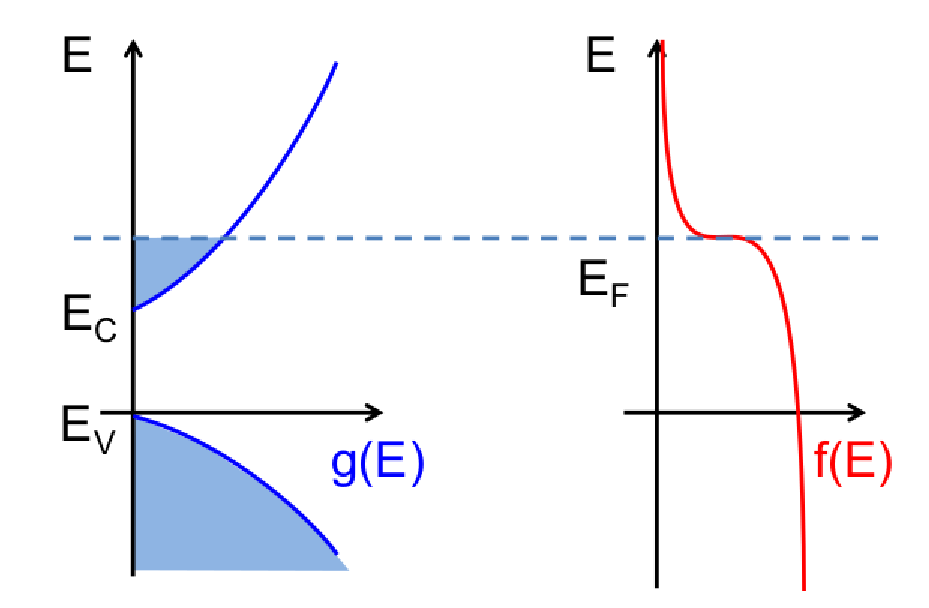
\includegraphics[width=.45\textwidth]{SemiconductorModel/BandeMetalli.eps}}
\psp{5}
\subfloat[][Insulator]
{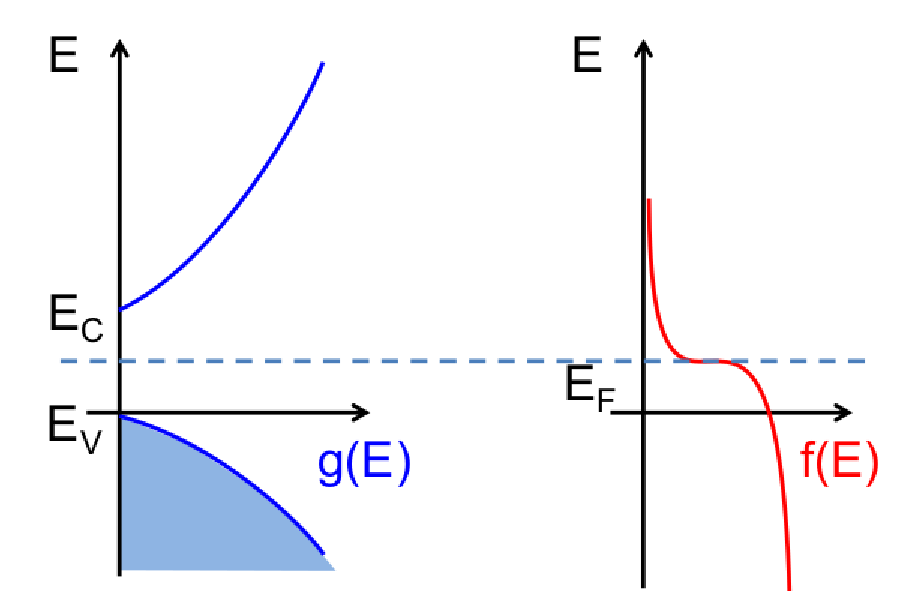
\includegraphics[width=.45\textwidth]{SemiconductorModel/BandeSemiconduttori.eps}}
\caption{Two typical examples of state density occupation (g(E)) and probability distribution (f(E)).  }
\end{figure}

Because in silicon the band gap is on the order of 1 [eV], at room temperature a small fraction of the electrons are excited into the conduction band, leaving behind vacancies (called \textit{holes}) in the valence band.
In contrast, an insulator has a much larger forbidden gap making room-temperature conduction virtually impossible, while metals have partially filled conduction bands even at absolute zero temperature, this make them good conductors at any temperature. 

A suitable formulation of che carrier concentration which is given, for electrons, by the follow integral:
\begin{equation}
\label{eq: carrier densiy integral}
n = \int_{E_c}^\infty g(E)f(E) \, dE
\end{equation}
With $g(E)dE$ we indicate the number of electronic states per unit volume with an energy between $E$ and $E+dE$ in the conduction band and $f(E)$ is a suitable probability ditribution.

The energy distribution of electrons in a solid is governed by the laws of Fermi-Dirac statistics. For a system in thermal equilibrium, the principal result of these statistics is the \textit{Fermi-Dirac distribution function}, which gives the probability that an electronic state at energy E is occupied by an electron,
\begin{equation}
\label{eq: fermi dirac distribution}
f_D(E) = \dfrac{1}{1+exp\left(\dfrac{E-E_f}{k_BT}\right)} 
\end{equation}
here $k_B=1.38\times10^{-23}[J/K]$ is Boltzmann's constant, $T$ is the absolute temperature and $E_f$ is the \textit{Fermi level}.

\begin{Definizione}
The Fermi level ($E_f$) is the energy at which the probability of occupation of an energy state by an electron is exactly one-half.
\end{Definizione}

In most cases when the energy is at least several $k_BT$ above or below the Fermi level \referenzaeq{eq: fermi dirac distribution} can be approximated with the Maxwell-Boltzmann statistics for classical particles, which read as follows:

\begin{equation}
\label{eq: maxwell distribution}
f_D(E)\simeq f_{MB}(E) = 
\begin{cases}
exp\left(-\dfrac{E-E_f}{KT}\right) & E\gg E_f \\
1-exp\left(-\dfrac{E_f-E}{KT}\right) & E \ll E_f
\end{cases}
\end{equation}

Fermi level plays an essential role in characterizing the equilibrium state of a stystem, it is important to keep in mind the sequent observation.

\begin{Osservazione}
When two systems are in thermal equilibrium with no current flow between them, their Fermi levels must be equal, in other words for a continuous region of metals and/or semiconductors in contact, the Fermi level at thermal equilibrium is flat (spatially constant throughout the region).
\end{Osservazione}

 In general \referenzaeq{eq: carrier densiy integral} is a Fermi integral of the order $1/2$ and must be evaluated numerically. In the case of non-degenerate semiconductor, Fermi levels stay at least $3KT/q$ below the edge of the conduction band (for holes we consider the same approximation above the valence band).  The Fermi-Dirac distribution can be approximated by the Maxwell-Boltzmann distribution and \referenzaeq{eq: carrier densiy integral} can be solved in the analytically way, obtaining,

\begin{align}
n & = N_c exp\left(-\dfrac{E_c-E_f}{KT}\right) \label{eq: n density fd}\\
p & = N_v exp\left(-\dfrac{E_f-E_v}{KT}\right)  \label{eq: p density fd}
\end{align}

where $N_c$ and $N_v$ are the \textit{effective density of states}.
In intrisic semiconductor $n=p$ and the \textit{intrinsic Fermi level} $E_i$ can be calculated using equations \referenzaeq{eq: n density fd} and \referenzaeq{eq: p density fd} as:

\begin{equation}
\label{eq: midgap equilibrium}
E_i=E_f=\dfrac{E_c+E_v}{2} - \dfrac{KT}{2}ln\left(\dfrac{N_c}{N_v}\right)
\end{equation}

By replacing \referenzaeq{eq: midgap equilibrium} in \referenzaeq{eq: n density fd} we have the expression of the intrinsic carrier concentration $n_i=n=p$:


\begin{equation}
\label{eq: ni equilibrium NcNv}
n_i = \sqrt{N_cN_v}exp\left(-\dfrac{E_g}{2KT}\right)
\end{equation}

\begin{Osservazione}
Since the thermal energy, $k_BT$ is muc smaller than the usual semiconductor bandgap $E_g$, the intrinsic Fermi level is very close to the midpoint between the conduction band and the valence band.
\end{Osservazione}

Equations \referenzaeq{eq: n density fd} and \referenzaeq{eq: p density fd} can be rewritten in terms of the intrinsic carrier density ($n_i$) and energy ($E_i$) :

\begin{align}
n & = n_i exp\left(\dfrac{E_f-E_i}{KT}\right) \label{eq: n density mb}\\
p & = n_i exp\left(\dfrac{E_i-E_f}{KT}\right)  \label{eq: p density mb}
\end{align}

Finally we remark a fundamental and useful relation holds at the thermical equilibrium

\begin{equation}
\label{eq: legge di azione di massa}
np=n_i^2
\end{equation}

this relation is usually note as \textit{mass action law}.

One of the most used graphical tool for the anlysis of the functionality of devices is the band diagram \figref{fig: band diagram}, which summarizes the informations presented above.
\begin{figure}[!h]
\centering
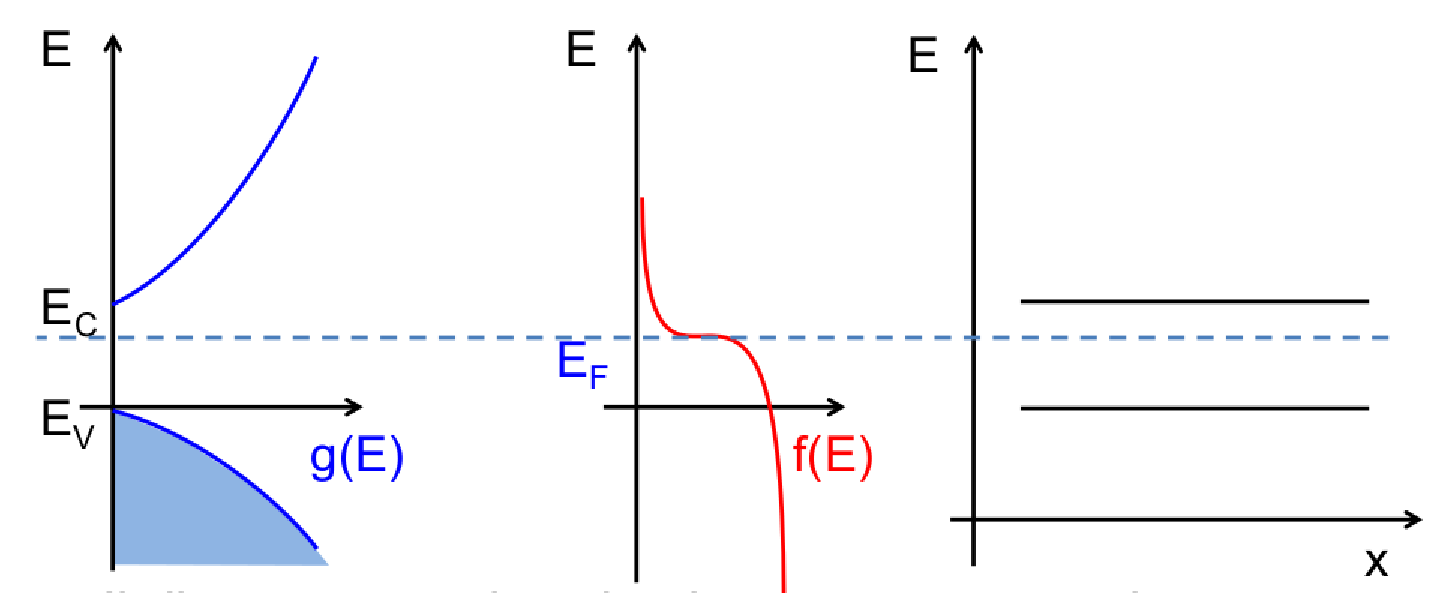
\includegraphics[width=.8\textwidth]{SemiconductorModel/DiagrammaBande.eps}
\caption{Construction of tha band diagram.}
\label{fig: band diagram}
\end{figure}

\subsection{Extrinsic semiconductor}
At room temperature intrinsic semiconductor has an extremely low free-carrier concentration, therefore, its resistivity is very high. In order to make semiconductor a better conductor it's usual add impurities atoms which introduce additional energy levels in the forbidden gap: these impurities are easily ionized adding either electrons to the conduction band or holes to the valence band. Here the electrical conductivity is dominated by the type and concentration of the impurity atoms.

In the case of silicon two are the types of impurities which are electrically active: those from column V such as arsenic or phosphorus, and those from column III such as boron or indium.

A column-V atom in a silicon lattice tends to have one extra electron loosely bonded after forming covalent bonds with other silicon atoms. In most cases, the thermal energy at room temperature is sufficient to ionize the impurity atom and free the extra electron to the conduction band. Such type of impurities are called \textit{donors}; they become positively charged when ionized. Silicon material doped with column-V impurities or donors is called \textit{n-type} silicon.

A column-III impurity atom in a silicon lattice tends to be deficient by one electron when forming covalent bonds with other silicon atoms. Such an impurity atom can also be ionized by accepting an electron from the valence band, which leaves a free-moving hole that contributes to electrical conduction. These impurities are called \textit{acceptors}: they become negatively charged when ionized. Silicon material doped with column-III impurities or acceptors is called \textit{p-type} silicon.

A p-type or an n-type is named as \textit{extrinsic} silicon.
In terms of the energy-band diagrams, donors add allowed electron states in the bandgap close to the conduction-band edge, while acceptors add allowed states just above the valence-band edge.

In contrast to intrinsic silicon, the Fermi level in an extrinsic silicon is not located at the midgap. The Fermi level in n-type silicon moves up towards the conduction band while in p-type silicon moves down towards the valence band.
The exact position of the Fermi level depends on both the ionization energy and the concentration of dopants. For example, for an n-type material with a donor impurity concentration, $N_d$, the charge neutrality condition requires that
\begin{equation}
\label{eq: equilibrium charge in n-type}
n = N_d^+ + p
\end{equation}
 where $N_d^+$ is the density of ionized donors.  Similarly for a p-type material with acceptor impurity concentration $N_a$ we have
\begin{equation}
\label{eq: equilibrium charge in p-type}
p = N_a^- + n
\end{equation}
 
 For the sake of simplicity we consider in this work that at room temperature all impurties are ionized ($N_d = N_d^+$ and $N_a = N_a^-$). Typcally the magnitude of impurities is between $10^{16}\ast 10^{20} [cm^{-3}]$, while the usual intrinsic carrier concentration is almost $10^{10}[cm_3]$, for this reason we can approximate the equilibrium densities concentration:
  
\begin{equation}
\begin{array}{ll}
n \simeq N_d & p \simeq \dfrac{n_i^2}{N_d} \\ \\
p \simeq N_a & n \simeq \dfrac{n_i^2}{N_a}
\end{array}
\end{equation}

 Take into account this approximation and substituting \referenzaeq{eq: n density fd} and \referenzaeq{eq: p density fd} in \referenzaeq{eq: equilibrium charge in n-type} and \referenzaeq{eq: equilibrium charge in p-type}, solving the algebraic equationwe have
 
 \begin{align}
 E_c-E_f = KTln\left(\dfrac{N_c}{N_d}\right)  \label{eq: Ef in n-type}\\
 E_f-E_v= KTln\left(\dfrac{N_v}{N_a}\right) \label{eq: Ef in p-type}
 \end{align}

Equation \referenzaeq{eq: legge di azione di massa} is indipendent of the dopant type and Fermi level position.
Instead of using $N_c$, $N_v$ and referring to $E_c$ and $E_v$ equation \referenzaeq{eq: Ef in n-type} and \referenzaeq{eq: Ef in p-type} can be written in a more useful form in terms of $n_i$ and $E_i$ defined by equations \referenzaeq{eq: ni equilibrium NcNv} and \referenzaeq{eq: midgap equilibrium}:

 \begin{align}
 E_f-E_i = KTln\left(\dfrac{N_d}{n_i}\right)  \label{eq: Ef in n-type Ei} \\
 E_i-E_f = KTln\left(\dfrac{N_a}{n_i}\right)  \label{eq: Ef in p-type Ei} 
 \end{align}

\begin{Osservazione}
The distance between the Fermi level and the intrinsic Fermi level near the midgap is a logarithmic function of doping concentration.
\end{Osservazione}

As a consequences:
\begin{itemize}
\item non linearity relations between potential and desities,
\item exponential dependence of densities from potential.
\end{itemize}

\begin{figure}[!h]
\centering
\subfloat[][n-type]
{\begin{tikzpicture}
[scale=1.0]
\def\Ecxa{0.0}
\def\Ecya{2}
\def\Ecxb{3}
\def\Ecyb{2}

\def\Evxa{\Ecxa}
\def\Evya{0}
\def\Evxb{\Ecxb}
\def\Evyb{0}

\def\Efxa{\Ecxa}
\def\Efya{1.7}
\def\Efxb{\Ecxb}
\def\Efyb{1.7}

\def\Eixa{\Ecxa}
\def\Eiya{1}
\def\Eixb{\Ecxb}
\def\Eiyb{1}

\node at (\Ecxb+0.5,\Ecyb){$E_C$};
\node at (\Evxb+0.5,\Evyb){$E_V$};
\node at (\Efxa-0.5,\Efya){$E_f$};
\node at (\Eixa-0.5,\Eiya){$E_i$};

\draw[ultra thick](\Ecxa,\Ecya)--(\Ecxb,\Ecyb);
\draw[ultra thick](\Evxa,\Evya)--(\Evxb,\Evyb);
\draw[ultra thick,dashed](\Efxa,\Efya)--(\Efxb,\Efyb);
\draw[dashed](\Eixa,\Eiya)--(\Eixb,\Eiyb);
\end{tikzpicture}}
\psp{20}
\subfloat[][p-type]
{\begin{tikzpicture}
[scale=1.0]
\def\Ecxa{0.0}
\def\Ecya{2}
\def\Ecxb{3}
\def\Ecyb{2}

\def\Evxa{\Ecxa}
\def\Evya{0}
\def\Evxb{\Ecxb}
\def\Evyb{0}

\def\Efxa{\Ecxa}
\def\Efya{0.3}
\def\Efxb{\Ecxb}
\def\Efyb{0.3}

\def\Eixa{\Ecxa}
\def\Eiya{1}
\def\Eixb{\Ecxb}
\def\Eiyb{1}

\node at (\Ecxb+0.5,\Ecyb){$E_C$};
\node at (\Evxb+0.5,\Evyb){$E_V$};
\node at (\Efxa-0.5,\Efya){$E_f$};
\node at (\Eixa-0.5,\Eiya){$E_i$};

\draw[ultra thick](\Ecxa,\Ecya)--(\Ecxb,\Ecyb);
\draw[ultra thick](\Evxa,\Evya)--(\Evxb,\Evyb);
\draw[ultra thick,dashed](\Efxa,\Efya)--(\Efxb,\Efyb);
\draw[dashed](\Eixa,\Eiya)--(\Eixb,\Eiyb);
\end{tikzpicture}}
\caption{Band diagrams of estrinsic silicon.}
\label{fig: Band diagrams of estrinsic silicon}
\end{figure}

\subsection{Densities at nonequilibrium condition}

In VLSI device operation a nonequilibrium sistuations is often possible: the densities of one or both types of carriers depart from their equilibrium values given by \referenzaeq{eq: n density mb} and \referenzaeq{eq: p density mb}.
In particular, the minority carrier concentration can be easily overwhelmed by injection from neighboring regions. Under these circumstances, while the electrons and holes are in local equilibrium with themselves, they are not in equilibrium with each other. In order to extend the relationship between Fermi level and densities discussed above, we can introduce separate Fermi levels for electrons and holes. They are called \textit{quasi Fermi levels} defined as $E_{fn}$ and $E_{fp}$ replacing equation \referenzaeq{eq: n density mb} and \referenzaeq{eq: p density mb}:

\begin{align}
n & = n_i exp\left(\dfrac{E_{fn}-E_i}{k_BT}\right) \label{eq: non eq n density mb}\\
p & = n_i exp\left(\dfrac{E_i-E_{fp}}{k_BT}\right)  \label{eq: non eq p density mb}
\end{align}

In non equilibrium condition quasi Fermi levels have a similar physical interpretation in terms of the state occupancy as the Fermi level.
\begin{Osservazione}
The electron density in the conduction band can be calculated using $E_{fn}$, and the hole density in the valence band using $E_{fp}$.
\end{Osservazione}

\subsection{Carrier transport in semiconductor}

Carrier transport or current flow in silicon is driven by two different mechanisms:
\begin{itemize}
\item the \textbf{drift} of carriers, which is caused by the presence of an electric field;
\item the \textbf{diffusion} of carriers, which is caused by and electron or hole concentration gradient.
\end{itemize}

\subsubsection{Drif current - Ohm's law}

When an electric field is applied to a media, the free carriers are accelerated and acquire a drift velocity superimposed upon their random thermal motion.

\begin{Osservazione}
The drift velocity of holes ($h$) is in the direction of the applied field, and the drift velocity of electrons ($e$) is opposite to the field.
\end{Osservazione}

The velocity of the carriers does not increase indefinitely under field acceleration, since they are scattered frequently and lose their acquired momentum after each collision.
During their motion throughout the lattice structure, carriers travel at an average speed definded as
\begin{equation}
\label{eq: velocities}
\vect{v}_d^e = - \dfrac{q\vect{E}\tau_e}{m_e}  \psp{20} 
\vect{v}_d^h = + \dfrac{q\vect{E}\tau_h}{m_h}
\end{equation}

where $q=1.602e^{-19}[C]$ is the elementary charge, $\vect{E}$ the electric field, $\tau_\eta$ the average time of flight of the carrier between two consecutive interactions with the atoms of the lattice and $m_\eta$ is the effective mass.
The coefficient $q\tau_\eta / m_\eta$ characterizes how quickly a carrier can move through the lattice and it's well known as carrier mobility $[m^2V^{-1}s^{-1}]$.
In general, to include different contributions to the mobility \textit{Matthiessen's rule} is used:
\begin{equation}
\dfrac{1}{\mu} = \dfrac{1}{\mu_L} + \dfrac{1}{\mu_I} + \cdots
\end{equation}
where $\mu_L$ and $\mu_I$ correspond to the lattice and impurity scattering limited components of mobility (for a more detailed description of mobility models see \cite{ModernVLSIdevices}). 

Therefore the drift electron, hole, current density, reads as follows:

\begin{align}
\vect{J}_n =& -qn\vect{v}_d^n = qn\mu_n\vect{E}   = \sigma_n\vect{E} \label{eq: drift electron} \\ 
\vect{J}_p =& +qp\vect{v}_d^p = qp\mu_p\vect{E} = \sigma_p\vect{E} \label{eq: drift hole}
\end{align}

The scalar coefficient $qn\mu_n(qp\mu_p)$ is often summerized by the electron (hole) conductivity $\sigma_n(\sigma_p)$. 

Relations \referenzaeq{eq: drift electron} and \referenzaeq{eq: drift hole} expresses the well known \textit{Ohm' law} stating that the current density is directly proportional to the applied electric field.


\subsubsection{Diffusion current - Fick's law}

In semiconductor devices it's usual have different profiles of dopant in order to allow particular behaviors, this implies a not uniform concentration of carriers which they also diffuse as a result of the concentration gradient. This leads to an additional current contribution accordingly to the \textit{Fick's law}:
\begin{align}
\vect{J}_n = -D_n(-q\nabla n) \label{eq: diff electron}\\
\vect{J}_p = -D_p(+q\nabla p) \label{eq: diff hole}
\end{align}

The proportionally constants $D_n$ and $D_p$ are called the electron and hole diffusion coefficients and have units of $[cm^2s^{-1}]$. Physically, both drift and diffusion are closely associated with the random thermal motion of carriers and their collisions with the silicon lattice in thermal equilibrium. A simple relationship between the diffusion coefficient and the mobility is the well known \textit{Einstein relation}:
\begin{equation}
D_\eta = \dfrac{k_BT}{q}\mu_\eta
\end{equation}

\subsubsection{Drift-Diffusion transport equations}
\label{subsub:driftdiffusion transport}

By considering \referenzaeq{eq: drift electron}, \referenzaeq{eq: drift hole}, \referenzaeq{eq: diff electron} and \referenzaeq{eq: diff hole}, the total electron and hole current densities are:

\begin{align}
\vect{J}_n &= qn\mu_n\vect{E} + qD_n\nabla n  \label{eq: drift diff electron}\\ 
\vect{J}_p &= qp\mu_p\vect{E} - qD_p \nabla p \label{eq: drift diff hole}
\end{align}
The total conduction current density is $\vect{J}=\vect{J}_n+\vect{J}_p$.

We remark that these constitutive laws can be rewritten in two other ways highlighting different physical explanations of the same phenomenon. Moreover these reinterpreations  give different start points for the discrete solver algorithm.

Considering that electric field is related to the scalar potential as:
\begin{equation}
\label{eq: relazione pot electric}
\vect{E}  = -\nabla \varphi
\end{equation}

the current densities can be :

\begin{align*}
\vect{J}_n &= -qn\mu_n\left(\nabla \varphi - \dfrac{k_BT}{qn}\nabla n \right)\\ 
\vect{J}_p &= -qp\mu_p\left(\nabla \varphi+ \dfrac{k_BT}{qp} \nabla p \right)
\end{align*}

Considering equations \referenzaeq{eq: non eq n density mb} and \referenzaeq{eq: non eq p density mb} the above can be written as:

\begin{align}
\vect{J}_n = -qn\mu_n\nabla \varphi_n \\
\vect{J}_p = -qn\mu_p\nabla \varphi_p 
\end{align}

With these equations we underlying an important aspect which occur in semiconductor material:
\begin{Osservazione}
The current density is proportional to the gradient of the quasi Fermi potential.
\end{Osservazione}

The third way to represent the current density is based on \textit{Slotboom variables}. In 1973 Jan Slotboom proposed this change in variables for the two-dimensional numercal simulation of a bipolar transistor:

\begin{align}
u_n &= n_iexp\left(-\dfrac{\varphi_n}{V_{th}} \right) \label{eq: un slotboom} \\
u_p &= n_iexp\left(\dfrac{\varphi_p}{V_{th}} \right) \label{eq: up slotboom} 
\end{align}

where $V_{th}=k_BT/q$. Using the above equations into \referenzaeq{eq: drift diff electron} and \referenzaeq{eq: drift diff hole} we obtain:

\begin{align}
\vect{J}_n &= qD_n exp\left(\dfrac{\varphi}{V_{th}}\right) \nabla u_n \label{eq: Jn slotboom} \\
\vect{J}_p &= -qD_p exp\left(-\dfrac{\varphi}{V_{th}}\right)  \nabla u_p 
\end{align}

This interpretation results is:
\begin{Osservazione}
The drift-diffusion current density in a semiconductor, is a totally diffusive flux of a new kind of carrier and diffusivity coefficient. 
\end{Osservazione}


\section{Drift Diffusion Model for semiconductor}
\label{section: dd model for semi}

Simulations on integrated devices works on several different scale, the \textit{Drift Diffusion model} (DD) is the most widely used mathematical tool for industrial simulaiton of semiconductor devices. In this section we'll show how is possible to deduce the DD model.

\subsection{Drift Diffusion formulation}
 The system of Maxwell equations describes the propagation of electromagnetic signal in a medium:

\begin{align}
\nabla \times \vect{H} & =  \vect{J} + \dfrac{\partial \vect{D}}{\partial t} \label{eq: magnetic equation} \\ 
\nabla \times \vect{E} & =  - \dfrac{\partial \vect{B}}{\partial t} \label{eq: ampere law}\\ 
\nabla \cdot \vect{D} & =  \rho \label{eq: gauss law}\\ 
\nabla \cdot \vect{B} &  =  0 \label{eq: no magetic charge law}
\end{align}

we complete the system with the following set of constitutive laws that characterize the electromagnetic properties of the medium:

\begin{equation}
\begin{array}{rcl}
\vect{D} & = & \epsilon \vect{E} \\
\vect{B} & = & \mu_m \vect{H} \label{eq: magnetic costitutive}
\end{array}
\end{equation}

where $\epsilon$ is the material dielectric permettivity $[F cm^{-1}]$ and $\mu_m$ is the magnetic permeability $[H cm^{-1}]$. Since $\nabla \cdot (\nabla \times \vect{A})=0$ for any vector $\vect{A}$, \referenzaeq{eq: no magetic charge law} is satisfied by introducing a vector potential $\vect{A}$ such that $\vect{B}= \nabla \cdot \vect{A}$. We replace it in \referenzaeq{eq: ampere law} and we obtain

\begin{equation}
\nabla \times \left( \vect{E} + \dfrac{\partial \vect{A}}{\partial t} \right) = 0.
\end{equation}

From this we can state that exist a scalar potential $\varphi$ such that

\begin{equation}
\label{eq: potenziale scalare}
\vect{E} + \dfrac{\partial \vect{A}}{\partial t} = -\nabla \varphi
\end{equation}


We multiply \referenzaeq{eq: potenziale scalare} by $\epsilon$, we apply the divergence operator and we obtain using \referenzaeq{eq: relazione pot electric}, \referenzaeq{eq: magnetic costitutive} and \referenzaeq{eq: gauss law}

\begin{equation}
\rho + \dfrac{\partial \vect{A}}{\partial t}  = -\nabla \cdot (\epsilon \nabla \varphi)
\end{equation}

We now assume that $\dfrac{\partial \vect{A}}{\partial t} = 0$ (quasi static approximation) and we obtain the \textit{Poisson Equation}

\begin{equation}
\label{eq: Poisson equation}
\nabla \cdot (\epsilon \nabla \varphi) = \rho.
\end{equation} 
	
	We apply the divergence operator on the equation \referenza{eq: magnetic equation}  and we get the \textit{Continuity Equation}

\begin{equation}
\dfrac{\partial \rho}{\partial t} + \nabla \cdot \vect{J}  =  0 \end{equation} 




To close the above system we need to specify the mathematical form of the electric charge density ($\rho$) and the electric conduction current density ($\vect{J}$).
As we introduced in the preview section, devices are usually formed by extrinsic semiconductor and this causes the presence in the lattice of two kind of charge:

\begin{itemize}
\item free charge ($\rho_{free}$) (free electron and holes carriers),
\item fixed charge ($\rho_{fixed}$) (ionoized dopant impurities).
\end{itemize} 

\begin{equation}
\label{eq: charge balance}
\rho = \underbrace{q(p-n)}_{\rho_{free}} +\underbrace{q(N_D^+-N_A^-)}_{\rho_{fixed}}
\end{equation}

 Notice that we assume $N_D^+$ and $N_A^-$ time invariant ($\partial N_D^+ / \partial t=\partial N_A^- / \partial t = 0$).

 Accordingly with the preview hypotesis and replacing \referenzaeq{eq: charge balance}, \referenzaeq{eq: drift diff electron} and \referenzaeq{eq: drift diff hole}, we can split the continuity equation into the contribute of electrons and holes, the DD model formulation looks as follows:
 
\begin{equation}
\label{eq: full problem}
\left\{
\begin{array}{rcl}
\nabla \cdot (-\epsilon \nabla \varphi) & = & q(p-n+N_D^+-N_A^-)\\ \\
-q\dfrac{\partial n}{\partial t} + \nabla \cdot ( - q\mu_n n \nabla \varphi + qD_n \nabla n )& = & qR\\ \\
q\dfrac{\partial p}{\partial t} + \nabla \cdot (- q\mu_p p \nabla \varphi - qD_p \nabla p )& = & -qR 
\end{array}
\right.
\end{equation}

The system is an incompletely parbolic initial value/boundary problem in three scalar unkown dependent variables $\varphi(\vect{x},t)$, $n(\vect{x},t)$ and $p(\vect{x},t)$. Notice that the problem is a nonlinearly coupled system of PDE's, because of the presence of the drift terms ($n\nabla \varphi$ and $p \nabla 	\varphi$). 

From Maxwell equations we are able to guarantee only that $\vect{J}$ is a solenoidal field, we can't say nothing about the properties of $\vect{J_n}$ and $\vect{J_p}$. We can interpret $R(\vect{x},t)$ as the net rate of generation and recombination.

The stationary form can be easily derivate from \referenzaeq{eq: full problem} by not considering the temporal derivative.

%\begin{equation}
%\label{eq: stationary problem}
%\left\{
%\begin{array}{rcl}
%\nabla \cdot (-\epsilon \nabla \varphi) & = & q(p-n+N_D^+-N_A^-) \\ \\
%\nabla \cdot ( - q\mu_n n \nabla \varphi + qD_n \nabla n )& = & qR \\ \\
%\nabla \cdot (- q\mu_p p \nabla \varphi - qD_p \nabla p )& = & -qR
%\end{array}
%\right.
%\end{equation}




\subsection{Generation and Recombination phenomenon}
\label{subsection: RG}

The modelling of $R(\vect{x},t)$ is one of the most important feature due to the important role in determining the current-voltage characteristic of devices.
 
It's important to keep in mind that electrons and holes are in continuos fluctuation due to their thermal energy, but the macroscopic result of such a process at equilibrium is that the net recombination rate is identically zero at each point and at each time level. Therefore our interest is to analyze the deviations from this condition. 

In every moment the system try to mantain the equilibrium, so it's important underlying that the response with a recombination event happens in order to neutralize an excess of charge, while generation event are usually due to thermal agitation or an external input source.

The phenomenological model for the net recombination rate $R$ is often given by the sequent formulation:
\begin{equation}
\label{eq: generic RG}
R(n,p) = (pn-n_i^2)F(n,p)
\end{equation}
where $F$ is a function modelling the specific recombination/generation (R/G) event.

In the following we present the classical theory about three kind of contribute. 

\subsubsection{Shockley-Read-Hall recombination (SRH)}

Electron and hole generation and recombination can take place directly between the valence band and the conduction band, or inderactly via trap centers in the energy gap (we indicate with $E_T$ the energy level at where these traps live). The latter category includes Shockley-Read-Hall phenomena (SRH), more precisely SRH rate is a two-particle process which matematically expresses the probality that:
\begin{itemize}
\item[$R_{SRH}$] an electron in the conduction band neutralizes a hole at the valence band through the mediation of an unoccupied trapping level located in the energy gap,
\item[$G_{SRH}$] an electron is emitted from the valence band to the conduction band, through he mediation of an unoccupied trapping level located in the energy gap.
\end{itemize}

The following expression is usually employed for the modulating function $F$:

\begin{equation}
F_{SRH}(n,p) = \dfrac{1}{\tau_n\left(p+n_i cosh\left(\dfrac{E_T}{k_BT} \right) \right)+\tau_p\left(n+n_i cosh\left(\dfrac{E_T}{k_BT}\right) \right)}
\end{equation}

the quantiaties $\tau_n$ and $\tau_p$ are called \textit{carrier lifetimes} and are phisically defined as the reciprocals of the capture rates per single carrier associated with the energy trap distribution within the semiconductor energy gap. Their typical order of magnitude lies in the range $10^{-3}\mu s\div 1 \mu s$.

\begin{table}[!h]
\centering
\begin{tabular}{cccc}
\toprule
Parameter & Unit & Electrons & Holes \\
\midrule
$\tau$ & s & $1.0\times 10^{-5}$ & $3.0 \times 10^{-6}$\\
$E_T$ & eV & 0.0 & 0.0\\
\bottomrule
\end{tabular}
\caption{List of parameters in the electron and hole mobility models including scattering from lattice thermal vibrations}
\end{table}

\subsubsection{Auger recombination (AU)}

Auger R/G is a three-particle process and take place directly between the valence band and the conduction band. We distinguish four cases which depend to the kind of carriers involved in the phenomena:
\begin{itemize}
\item[$R_{AU}^{2n,1p}$] a high-energy electron in the conduction band moves to the valence band where it neutralizes a hole, transmitting the excess energy to another electron in the conduction band;
\item[$G_{AU}^{2n,1p}$] an electron in the valence band moves to the conduction band by taking the energy from a high energy electron in the conduction band and leaves a hole in the valence band;
\item[$R_{AU}^{2p,1n}$] an electron in the conduction band moves to the valence band where it neutralizes a hole, transmitting the excess energy to another hole in the valence band;
\item[$G_{AU}^{2p,1n}$] an electron in the valence band moves to the conduction band by taking the energy from a high energy hole in the valence band and leaves a hole in the valence band.
\end{itemize}

The following expression is usually employed for the modulating function $F$:

\begin{equation}
F_{AU}(n,p) = C_nn+C_pp
\end{equation}

where the quantitaties $C_n$ and $C_p$ are the so called  Auger capture coefficients tipically of the order of magnitude of $10^{-25}[cm^6s^{-1}]$.
Note that Auger R/G is relevant only when both carrier densities attain high values.

\begin{table}[!h]
\centering
\begin{tabular}{ccc}
\toprule
Parameter & Unit & Magnitude \\
\midrule
$C_n$ & $cm^6s^{-1}$ & $2.9 \times 10^{-31}$ \\
$C_p$ & $cm^6s^{-1}$ & $1.028 \times 10^{-31}$ \\
\bottomrule
\end{tabular}
\caption{List of parameters in the electron and hole Auger generation/recombination model.}
\end{table}

\subsubsection{Impact ionization (II)}

The impact ionization mechanism is a three-particle generation  process and it is dissimilar from the previously phenomenon because we can't express its contribute with a relation like \referenzaeq{eq: generic RG}. The high energy carrier generation is triggered by the presence of very high electric fields. Due to these fields an electron could gains enough energy to excite an electron-hole pair out of a silicon lattice bond. Then the process can be repeated until an avalanche of generated carriers is produced within the region.
There are several different models for the II generation, inside our code we implemented the van Overstraeten - de Man \textcolor{red}{referenza manuale sdevice} model based on the Chynoweth law \textcolor{red}{referenza dentro sdevice}:
\begin{equation}
G_{II}(n,p)= \alpha_n n |\vect{v}_n| + \alpha_p p |\vect{v}_p|
\end{equation}

where:

\begin{equation}
\alpha(E_{ava}) = \gamma exp\left(-\dfrac{\gamma b}{E_{ava}} \right)
\end{equation} 
\begin{equation}
\gamma = \dfrac{tanh\left(\dfrac{\hbar \omega_{op}}{2k_BT_0} \right) }{tanh\left(\dfrac{\hbar \omega_{op}}{2k_BT} \right)}
\end{equation}

The factor $\gamma$ with the optical phono energy $\hbar \omega_{op}$ expresses the temperature dependence of the phonon gas against which carriers are accelerated.
$E_{ava}$ is the driving force which takes into account how the electric field influence the generation event. There are two possibilties to compute this quantity:
\begin{itemize}
\item compute the component of the elctrostatic field in the direction of the current
\begin{equation}
E_{ava}^{n,p} = \dfrac{\vect{E}\cdot\vect{J}_{n,p}}{||\vect{J}_{n,p}||}
\end{equation}
\item consider the module of the quasi fermi gradient
\begin{equation}
E_{ava}^{n,p} = |\nabla \varphi_{n,p}|
\end{equation}
\end{itemize}

\begin{table}[!h]
\centering
\begin{tabular}{ccccc}
\toprule
Parameter & Unit & Electrons & Holes  & Valid range of electric field\\
\midrule
$E_0$ & $V \, cm^{-1}$ & $4.0 \times 10^{5}$ & $4.0 \times 10^{5}$ & \\
$a_{high}$ & 1 & $7.03 \times 10^{5}$ & $6.71 \times 10^{5}$ & $E_0$ to $6.0 \times 10^{5}$\\
$a_{low}$ & 1 & $7.03 \times 10^{5}$ & $1.582 \times 10^{6}$ & $1.75 \times 10^{5}$ to $E_0$\\
$b_{high}$ & 1 & $1.231 \times 10^{6}$ & $1.693 \times 10^{6}$ & $E_0$ to $6.0 \times 10^{5}$\\
$b_{low}$ & 1 & $1.231 \times 10^{6}$ & $2.036 \times 10^{6}$ &$1.75 \times 10^{5}$ to $E_0$\\
$\hbar\omega_{op}$ & eV & 0.063 & 0.063\\
\bottomrule
\end{tabular}
\caption{List of parameters in the electron and hole of van Overstraeten-de Man model}
\end{table}

\subsection{Mobility models}

In the following section we illustrate the most commonly used phenomenological models to describe carrier mobilities. More precisely we want describe  the several mechanisms that characterize the average time of flight \referenzaeq{eq: velocities}.
Scattering phenomenon slow down the motion of carriers throughout the lattice and the three main physical principles governing these events are:
\begin{itemize}
\item interaction with the thermally generated vibrations of the silicon atoms;
\item presence of ionized dopant impurities in the crystal;
\item reduction to the velocity saturation at high electric fields.
\end{itemize}

\subsubsection{Scattering from thermal vibrations}


Intuitively, carrier mobility is to be a decreasing function of temperature, as we expect collisions to become more and more frequent as T gets higher. This idea is commonly represented using a simple power law of the form

\begin{equation}
\label{eq: mobility thermal}
\mu_\nu^L = \mu_\nu^0\left( \dfrac{T}{T_0}\right)^{-\beta_\nu} \psp{15} \nu = n,p
\end{equation}



where $\mu_\nu^0$ is the low-field mobility, $\beta_\nu$ are positive numbers and $T_0$ is a reference temperature typically $T_0=300[K]$.

\begin{table}
\centering
\begin{tabular}{cccc}
\toprule
Parameter & Unit & Electrons & Holes \\
\midrule
$\mu^0$ & $cm^2V^{-1}s^{-1}$ & 1417.0 & 470.5\\
$\beta$ & 1 & 2.5 & 2.2\\
\bottomrule
\end{tabular}
\caption{List of parameters in the electron and hole mobility models including scattering from lattice thermal vibrations}
\end{table}

\subsubsection{Scattering from Ionized Impurities}
Dopant ionized impurities represent local perturbations of the periodic distribution of silicon atoms. They strongly influence the carrier motion through electrostatic interaction, reducing the mobility of electrons and holes. The model used to simulate doping-dependent mobility in silicon was proposed by \textit{Masetti}:


\begin{equation}
\label{eq: mobility impurities}
\mu = \mu_{min1}exp\left( 	- \dfrac{P_c}{N_{tot}}\right)
 + \dfrac{\mu^L-\mu_{min2}}{1 + \left( \dfrac{N_{tot}}{C_r} \right)^{\alpha} } 
 - \dfrac{\mu_1}{1 + \left( \dfrac{C_s}{N_{tot}} \right)^{\beta} } 
\end{equation}

where $N_{tot} = N_D^+ + N_A^-$, $\mu_\nu^L$ is given by \referenzaeq{eq: mobility thermal}, $\mu_{min1}$ and $\mu_{min2}$  are a positive quantities representing the minimum value of $\mu$, $P_c$, $C_r$ and $C_s$ are reference doping values.


\begin{table}[!h]
\centering
\begin{tabular}{cccc}
\toprule
Parameter & Unit & Electrons & Holes \\
\midrule
$\mu_{min1}$ & $cm^2V^{-1}s^{-1}$ & 52.2 & 44.9\\
$\mu_{min2}$ & $cm^2V^{-1}s^{-1}$ & 52.2 & 0\\
$\mu_1$ & $cm^2V^{-1}s^{-1}$ & 43.4 & 29.0 \\
$P_c$ & $cm^{-3}$ & 0 & $9.23\times 10^{16}$\\
$C_r$ & $cm^{-3}$ &  $9.68\times 10^{16}$ & $2.23\times 10^{17}$ \\
$C_s$ & $cm^{-3}$ & $3.43\times 10^{20}$ & $6.10\times 10^{20}$\\
$\alpha$& 1 & 0.680 & 0.719  \\
$\beta$& 1 & 2.0 & 2.0 \\
\bottomrule
\end{tabular}
\caption{List of parameters in the electron and hole mobility models including scattering from ionized dopant impurities.}
\end{table}


\subsubsection{Veclocity saturation at high electric field}

Under the assumption of low electric field, mobilities are reasonably constant and the carrier drift velocity is proportional to the electric field. As the applied field strength increases, the above assumption is completely wrong as it would predict an unbounded carrier velocity in the material as $|\vect{E}| \rightarrow \infty$.
On the contrary, carrier scattering with lattice phonos produces a limitation to carrier velocity according to the following mathematical expression

\begin{equation}
\label{eq: velocity saturation}
\lim_{|\vec{E}| \to \infty} \mu |\vect{E}| = v_{sat}
\end{equation} 

A common adopted formula is the \textit{Canali model} with temperature dependent parameters

\begin{equation}
\label{eq: mobility canali}
\mu = \dfrac{\mu_{L}}{\left[ 1 + \left( \dfrac{\mu_{L}|\vect{E}|}{v_{sat}} \right)^{\beta}   \right]^{1/\beta}} 
\end{equation}
\vspace{0.5cm}
\begin{equation}
\label{eq: mobility canali beta}
v_{sat} = v_0exp\left( 	\dfrac{300}{T} \right)^{v_{exp}} 
\psp{15}
\beta= \beta_0 \left( \dfrac{T}{300} \right)^{\beta_{exp}}.
\end{equation}


\begin{table}[!h]
\centering
\begin{tabular}{cccc}
\toprule
Parameter & Unit & Electrons & Holes \\
\midrule
$v_0$ & $cm\,s^{-1}$ & $1.07\times 10^{7}$ & $8.37\times 10^{6}$\\
$v_{exp}$ & 1 & 0.87 & 0.52\\
$\beta_0$ & 1 & 1.109 & 1.213 \\
$\beta_{exp}$ & 1 & 0.66 & 0.17\\
\bottomrule
\end{tabular}
\caption{List of parameters in the electron and hole mobility models including scattering from velocity saturation.}
\end{table}


\clearpage
\section{Resolution of the system}

\subsection{Drawbacks of the Box Methods}
While the box method has become the standard technique for the discretization of the continuity equations, it suffers from several drawbacks arising from geometrical considerations. Satisfactory results can be obtained only for acute triangulations. Even one obtuse triangle can lead to a large spike in the solution of the equation.

In this form we can approach to the resolution of the problem only with a completely coupled Newton method. It's well known that there are several issues adopting this way of resolution:
\begin{itemize}
\item the jacobian matrix is often quite ill-conditioned and needs appropriate scaling and balancing in order to avoid problems associated with round-off error;
\item to ensure convergence of the Newton iterative process, it is particularly important to ensure a very good initial guess for the unknown variables;
\item dimension of the linearized problem is of the order of $N_{dofs}^3$ ($N_{dofs}$ is the number of degree of freedom used for the numerical approximation).
\end{itemize}

These considerations urges us to pursue an alternative approach: the decoupled Gummel Map.
First of all we have to introduce the Maxwell-Boltzamann approximation for the carriers:
\begin{equation}
\begin{array}{rcl}
n&=&n_iexp\left(\dfrac{\varphi-\varphi_n}{V_{th}}\right) \\
p&=&n_iexp\left(\dfrac{\varphi_p-\varphi}{V_{th}} \right)\\
\end{array}
\end{equation} 
Thanks to these expressions we are able to shift the nonlinearity on the poisson equation. Finally we obtain the following system:
\begin{equation}
\label{eq: gummel map system}
\left\{
\begin{array}{rcl}
\nabla \cdot (-\epsilon \nabla \varphi) + n_i\left( exp\left(\dfrac{\varphi-\varphi_n}{V_{th}}\right) - exp\left(\dfrac{\varphi_p-\varphi}{V_{th}}\right) \right) & = & q(N_D^+-N_A^-) \\ \\
-q\dfrac{\partial n}{\partial t} + \nabla \cdot ( - q\mu_n n \nabla \varphi + qD_n \nabla n )& = & qR\\ \\
q\dfrac{\partial p}{\partial t} + \nabla \cdot (- q\mu_p p \nabla \varphi - qD_p \nabla p )& = & -qR
\end{array}
\right.
\end{equation}

Referring on system \referenzaeq{eq: gummel map system} it's trivial introduce the Gummel Map algorithm:
\mybox{
Given $\varphi_n^{(0)}$ and $\varphi_p^{(0)}$, $\forall k$ until convergence:
\\
\begin{itemize}
\item Solve the Nonlinear Poisson Equation (NLP):
\begin{equation*}
\nabla \cdot (-\epsilon \nabla \varphi) + n_i\left( exp\left(\dfrac{\varphi-\varphi_n^{(k)}}{V_{th}}\right) - exp\left(\dfrac{\varphi_p^{(k)}-\varphi}{V_{th}}\right) \right)  =  q(N_D^+-N_A^-)
\end{equation*}
Set $\varphi^{(k)}=\varphi$.
\\
\item Solve the Linear Electron Contintuity Equation (LEC):
\begin{equation*}
-q\dfrac{\partial n}{\partial t} + \nabla \cdot ( - q\mu_n n \nabla \varphi^{(k)} + qD_n \nabla n ) = qR
\end{equation*}
Set $n^{(k)}=n$.
\\
\item Solve the Linear Hole Contintuity Equation (LHC):
\begin{equation*}
q\dfrac{\partial p}{\partial t} + \nabla \cdot (- q\mu_p p \nabla \varphi^{(k)} - qD_p \nabla p ) =  -qR
\end{equation*}
Set $p^{(k)}=p$.
\end{itemize}

}{Gummel Map}

Actually there are several methods to set up this algorithm and basically they depends on how we represent the conduction current density. Take for example this well-known change of variables proposed by the physicist Jan Slotboom:
\begin{equation}
\label{eq: slotboom formulas}
\begin{array}{rcl}
u_n & := & n_i exp\left(-\dfrac{\varphi_n}{V_{th}} \right)\\
u_p & := & n_i exp\left(\dfrac{\varphi_p}{V_{th}} \right) \\
\end{array}
\end{equation}
As a consequence we can reformulate \referenzaeq{eq: full problem} taking into account this interesting series of equivalences:
\begin{multline*}
\footnotesize
\vect{J_n}=
q\mu_n \left( - n \nabla \varphi + V_{th} \nabla \left( u_n exp\left(\dfrac{\varphi}{V_{th}} \right) \right) \right) \\ = 
q \mu_n \left(  -n \nabla \varphi + V_{th}\nabla u_n exp\left(\dfrac{\varphi}{V_{th}} \right) + n \nabla \varphi \right) \\ =
q D_n exp\left(\dfrac{\varphi}{V_{th}} \right) \nabla u_n 
\end{multline*}

The new Gummel Map algorithm read as follows:

\mybox{
Given $u_n^{(0)}$ and $u_p^{(0)}$, $\forall k$ until convergence:
\\
\begin{itemize}
\item Solve the Nonlinear Poisson Equation (NLP):
\begin{equation*}
\nabla \cdot (-\epsilon \nabla \varphi) + u_n^{(k)}exp\left(\dfrac{\varphi}{V_{th}}\right) - u_p^{(k)}exp\left(\dfrac{-\varphi}{V_{th}}\right) =  q(N_D^+-N_A^-)
\end{equation*}
Set $\varphi^{(k)}=\varphi$.
\\
\item Solve the Linear Electron Contintuity Equation (LEC):
\begin{equation*}
-q\dfrac{\partial u_nexp\left(\dfrac{\varphi^{(k)}}{V_{th}}\right)}{\partial t} + \nabla \cdot ( q D_n exp\left(\dfrac{\varphi^{(k)}}{V_{th}} \right) \nabla u_n ) = qR
\end{equation*}
Set $u_n^{(k)}=u_n$.
\\
\item Solve the Linear Hole Contintuity Equation (LHC):
\begin{equation*}
q\dfrac{\partial u_pexp\left(\dfrac{-\varphi^{(k)}}{V_{th}}\right)}{\partial t} + \nabla \cdot (q D_n exp\left(\dfrac{-\varphi}{V_{th}} \right) \nabla u_p ) =  -qR
\end{equation*}
Set $u_p^{(k)}=u_p$.
\end{itemize}

}{Gummel Map}



\section{Nonlinear Poisson Equation}
In this section we'll show how the NLP is resolved in the code. Many decisions have been taken on the management of the interface. Note that the electrostatic problem must be resolved on the whole domain and the right hand side changes from region to region.

\textcolor{blue}{Qui dipende da come vogliamo introdurre FEMOS...sarebbe carino far capire la scelta che è stata fatta di porre nei nodi di frontiera del silicio il valore della forzante e della reazione del silicio.Ma ovviamente questo discorso necessita una introduzione sui casi test.}

\subsection{Weak formulation}
Let us consider the linearized problem \textcolor{blue}{(qua ci vuole la referenza a quella linearizzata)} in a more generalized form which reads as follows:
\begin{equation}
\left\{
\begin{array}{rcll}
\nabla \cdot (-\epsilon \nabla \varphi) + \sigma^{(k)}(\vect{x}) \varphi & = &  f^{(k)}(\vect{x}) & \psp{15} in \psp{2} \Omega \\
\varphi & = & \varphi_D & \psp{15} on \psp{2} \Gamma_D \\
\nabla \varphi \cdot \vect{n} & = & 0 & \psp{15} on \psp{2} \Gamma_N
\end{array}
\right.
\end{equation}

For the sake of simplicity we summerize the reaction and force term in $\sigma$ and $f$, but we kept visible the iteration dependence.
The well-posedness of such problem is ensured by several (and reasonable) hypotesis:
\begin{itemize}
\item $\epsilon \in L^{\infty}(\Omega)$ and $\exists m$ s.t. $0 < m \leq \epsilon$ (a.e.) in $\Omega$;
\item  $\sigma \in L^{\infty}(\Omega)$ and $\exists m$ s.t. $0 < m \leq \sigma$ (a.e.) in $\Omega$.
\end{itemize}

We proceed with the classical displacement weak formulation.
Given $\varphi_D \in H^{1/2}(\Gamma_D)$ and $f \in L^2(\Omega)$ find $\varphi \in H^1(\Omega)$ such that 

\begin{equation}
\int_{\Omega} \epsilon \nabla \varphi \nabla v \, d\Omega + \int_{\Omega} \sigma^{(k)}\varphi v \, d\Omega = \int_{\Omega} f^{(k)}v \, d\Omega \psp{15} \forall v \in H^1_{\Gamma_D}(\Omega)
\end{equation}

\subsection{Numerical approximation}

\subsection{Damping}
\textcolor{blue}{Interessante fare vedere qualche grafico con qualche controllo della convergenza...}



\section{Continuity Equation}


\subsection{Weak formulation}
Without loss of generality we consider only the electron continuity equation (similar reasoning could be make for the hole continuity equation). Problem \textcolor{blue}{referenza al problema} is a classical diffusion-advection-reaction (DAR) problem written in conservative form. We will treat this PDE's equation likewise Poisson equation with the standard displacement weak formulation.

Be carefull about the right hand side: in the operation of many devices this term generates mass; this implies that a new reaction term is usually added in the left side of the equation:
\begin{equation}
R_n = \sigma n - f
\end{equation}

\begin{equation}
\left\{
\begin{array}{rcll}
\dfrac{\partial n}{\partial t} + \nabla \cdot ( - D_n \nabla n ) + \nabla \cdot ( \mu_n \nabla \varphi^{(k)} n )  + \sigma n & = & f  & \psp{15} in \psp{2} \Omega \\
n & = &  n_D & \psp{15} on \psp{2} \Gamma_D \\
\nabla n \cdot \vect{n} & = & 0 & \psp{15} on \psp{2} \Gamma_N
\end{array}
\right.
\end{equation}

Given $n_D \in H^{1/2}(\Gamma_D)$ and $f \in L^2(\Omega)$ find $n \in H^1(\Omega)$ such that:

\begin{equation}
\left\{
\begin{array}{rcll}
\dfrac{\partial n}{\partial t} + \nabla \cdot ( - D_n \nabla n ) + \mu_n \nabla \varphi^{(k)} \nabla n  + (\mu_n \Delta \varphi^{(k)} + \sigma) n & = & f  & \psp{15} in \psp{2} \Omega \\
n & = &  n_D & \psp{15} on \psp{2} \Gamma_D \\
\nabla n \cdot \vect{n} & = & 0 & \psp{15} on \psp{2} \Gamma_N
\end{array}
\right.
\end{equation}

with $\Gamma_D\cap\Gamma_N=\varnothing$, $\Gamma_D\cup\Gamma_N=\partial \Omega$ and where $\vect{n}$ is the outward normal vector on $\Omega$.
We respect the standard hypotesti for the wellposdness of the problem:
\begin{itemize}
\item $D_n \in L^{\infty}(\Omega)$ and $\exists \, m$ s.t. $0<m\leq D_n$ a.e. in $\Omega$;
\item $\sigma \in L^{\infty}(\Omega)$ and $\exists \, m$ s.t. $0<m\leq \sigma$ a.e. in $\Omega$;
\item $\mu_n \nabla \varphi \in (W^{1,\infty}(\Omega))^d$.
\end{itemize}

\textcolor{blue}{formulazione con tempo?}


\subsection{Numerical approximation}

\textcolor{blue}{Partiamo con una semidiscretizzazione spaziale e poi trattiamo anche quella temporale?}

\textcolor{blue}{Descrizione dettagliata (o meno?) del metodo implementato FVSG}

\section{Maximum discrete principle}
\textcolor{blue}{Scriviamo qualcosa in merito?Quanto approfondito?}


\section{The current calculation problem}

In many physical and engineering problems the real interesting variable of the conservation law is the flux in the domain or on specific surfaces and boundaries. The study of micro and nano electronics devices doesn't except this observation, in fact most of all models are oriented to obtain a satisfactory description of the current density.
 We know that the primal and not mixed formulation for  the continuity equation doesn't resolved  the flux density. The conseguence of this fact is a binding post-processing of the quantities computed in order to reconstruct the current density of electrons and holes.
It's evident which this part covers a lead role in the device simulation: 
as we are satisfied of the impressive results of the finite element scheme, it will be reather regrettable to lost the accuracy of our simulation during the computation of the current density.
About this question many academics propose different solutions and  the relative literature is boundless.
 
Tuttavia il problema ha vari livelli di complicazione:
3D problem
costi computazionali
conservazione flussi ortogonali

Quindi avere un metodo che soddisfi tutti i criteri non e banale

Cominciamo a descirvere la pietra miliare di tale argomento. 
 
 
\textcolor{blue}{Qua dobbiamo trovare un'introduzione che mette in luce i problemi di conto che escono fuori nel postprocessing del calcolo della corrente. Se davvero il problema fosse la non ottimale risoluzione del potenziale si potrebbero fare delle prove con il modulo mechanical (di fondo lo sforzo \`e assimiliabile alla densit\`a di corre potrebbero fare delle probe con float (occorre generalizzare il codice al tipo voluto lavoro lungo ma si pu\o fare))}

\subsection{Scharfetter Gummel method}

We remark the well known \textit{Scharfetter Gummel} equation for the carriers current density over the $k^{th}$ 1D element. It was proposed in 1969 by D. Scharfetter and H.K. Gummel (two scientists of Bell Labs). We point out some specific notation for the 1D case:

\begin{tikzpicture}
[scale=1.5]
\footnotesize
\def\SC{0.8}
\def\hx{8}
\def\hy{3}

%Solid line
\def\ax{0.5}
\def\ay{0}
\def\bx{3}
\def\by{0}

%Dash line
\def\cx{0}
\def\cy{0}
\def\dx{3.5}
\def\dy{0}

\def\Np{4}
\def\step{\bx/\Np-\ax/\Np}
%\tikzstyle{Normal}=[rectangle,draw=white];
\useasboundingbox (0,-1) rectangle (\hx,\hy);

\draw [dashed] (\cx,\cy)--(\ax,\ay);
\draw [dashed] (\bx,\by)--(\dx,\dy);
\draw (\ax,\ay)--(\bx,\by);
\draw [black,draw, fill=black] (\ax+0.15,\ay) circle [radius=0.05];
\draw [black,draw, fill=black] (\ax+0.15+1*\step,\ay) circle [radius=0.05];
\draw [black,draw, fill=black] (\ax+0.15+2*\step,\ay) circle [radius=0.05];
\draw [black,draw, fill=black] (\ax+0.15+3*\step,\ay) circle [radius=0.05];

\draw [thick] (\ax+0.15+1*\step+0.35,\ay+0.05) node[above]{\large $k$};
\draw [thick] (\ax+0.15+1*\step,\ay-0.1) node[below]{\large $n_{i}$};
\draw [thick] (\ax+0.15+2*\step,\ay-0.1) node[below]{\large $n_{i+1}$};

\node [right,text width=5cm] (texteig) at (\ax+0.15+1*\step,\ay+1.2){\large $\vect{E}$};

%Corpo
\draw (\ax+0.15+1*\step,\ay+1)--(\ax+2*\step-0.1,\ay+1);
\draw (\ax+0.15+1*\step,\ay+0.8)--(\ax+2*\step-0.1,\ay+0.8);
\draw (\ax+0.15+1*\step,\ay+1)--(\ax+0.15+1*\step,\ay+0.8);
%Punta
\draw (\ax+2*\step-0.1,\ay+1.05)--(\ax+0.15+2*\step,\ay+0.9);
\draw (\ax+2*\step-0.1,\ay+0.75)--(\ax+0.15+2*\step,\ay+0.9);

\draw (\ax+2*\step-0.1,\ay+1.)--(\ax+2*\step-0.1,\ay+1.05);
\draw(\ax+2*\step-0.1,\ay+0.8)--(\ax+2*\step-0.1,\ay+0.75);

\node [right,text width=5cm] (texteig) at (\dx+1,0.5){\large $\Delta\varphi^k = \varphi_{i+1} -\varphi_i$};

\end{tikzpicture}

\begin{equation}
\label{eq: scharfetter gummel 1D electron}
J_n^k=-q\frac{D_n}{h}
\left[ n_{i+1}\mathcal{B}\left(\frac{\Delta \varphi^k}{V_{th}}\right)- n_i\mathcal{B}\left(-\frac{\Delta \varphi^k}{V_{th}}\right)\right] 
\end{equation}

\begin{equation}
\label{eq: scharfetter gummel 1D hole}
J_p^k=-q\frac{D_p}{h}
\left[ p_{i+1}\mathcal{B}\left(-\frac{\Delta \varphi^k}{V_{th}}\right)- p_i\mathcal{B}\left(\frac{\Delta \varphi^k}{V_{th}}\right)\right] 
\end{equation} 


The extension of this formula for the 3D case is not trivial. We show the method for the computation of the current density of electrons (the extension for the current density of holes is quite similar).
We remark the quasi fermi formula for current density:
\begin{equation}
\label{eq: current density fermi}
\vect{J}_n=-q \mu_n n \nabla \varphi_n
\end{equation}
where $\varphi_n$ is the quasi fermi potential level. Let us write \referenzaeq{eq: current density fermi} in function of potential and in a canonic form:
\begin{equation}
\label{eq: current density canonic form}
\vect{J}_n\dfrac{ exp\left(\dfrac{\varphi_n-\varphi}{V_{th}}\right)}{q \mu_n n_i} + \nabla \varphi_n = 0
\end{equation}

Now consider a generic discretization for $\vect{J}_n$ and $\varphi_n$, for example finite element with $\mathbb{P}_1$ functions as bases (\textcolor{red}{vero che si pu´o scegliere qualsiasi discretizzazione con una qualsiasi base?}), we'll call these spaces $\left[ V_h \right]^d$ and $V_h$ (with $h$ we intend the step of discretization and $d$ is the dimension of simulation). We are able to test \referenzaeq{eq: current density canonic form} against $\vect{q}^h \in \left[ V_h \right]^d$, we choose three  different $\vect{q}^h$:

\begin{equation}
\label{eq: form of qh}
\vect{q}^h_{1,2,3} = \left\{ \begin{bmatrix} 1 \\ 0 \\ 0 \end{bmatrix}  \begin{bmatrix} 0 \\ 1 \\ 0 \end{bmatrix}  \begin{bmatrix} 0 \\ 0 \\ 1 \end{bmatrix}  \right\}
\end{equation}
We show the variational form for a generic element $K$ of the discretization:
\begin{equation}
\label{eq: variation form of current density}
\int_K \dfrac{ exp \left( \dfrac{\varphi_n-\varphi}{V_{th}} \right) }{q \mu_n n_i} \vect{J}_n^h \cdot \vect{q}^h_i \, dK
 + \int_K \nabla \varphi_n^h \cdot \vect{q}^h_i \, dK = 0 \psp{10} \forall i=1,2,3
\end{equation}

\textcolor{red}{La questione \`e: $\nabla \varphi_n^h \in \left[ V_h \right]^d$ ??. Possiamo dirlo sapendo che $\varphi_n^h \in V_h$ ??}

We know that $\nabla \varphi_n \in \mathbb{P}_0$ and without any approximation (except for the discretization) we obtain the sequent formula for the current density components:
\begin{equation}
\label{eq: first formula for J}
[\vect{J_n}]_i = - \mathbb{H}_K \left( q \mu_n n_i exp \left( \dfrac{\varphi-\varphi_n}{V_{th}} \right)  \right) \dfrac{\partial \varphi_n^h}{\partial x_i} \psp{5} i = 1...d \psp{5} \forall K \in \tau_h
\end{equation}
where $\mathbb{H}_K(f)$ is the armonic average on the elment $K$ of the function $f$.

Although resolve the armonic average with a comlete 3D integration may be expensive in calculation time and propably not necessary. One approximation of this integral would be pass from a 3D integration to 1D integration along one edge of the element $K$.
\begin{equation}
\label{eq: approzimation from 3D to edge}
\left(\dfrac{\int_K f^{-1} \, dK}{|K|} \right)^{-1} \simeq \left(\dfrac{\int_{e*} f^{-1} \, de}{|e^*|} \right)^{-1}
\end{equation}
  The approximation \referenzaeq{eq: approzimation from 3D to edge} is valid if we consider the correct edge.


Consider a quantity defined on the verteces:
\begin{equation}
\label{eq: differenza tra pot e qf}
\Phi := \varphi - 	\varphi_n
\end{equation}
which is the difference between the electrostatic potential and the quasi fermi potential level. Now for every element consider two vertices: $\vect{x}_m$ s.t. $\Phi(\vect{x}_m)=\Phi_m := min_K(\Phi)$ and $\vect{x}_M$ s.t. $\Phi(\vect{x}_M)=\Phi_M:=max_K(\Phi)$. Obviously it exists only one edge which connects these two points and on this one we perform the 1D integration \referenzaeq{eq: approzimation from 3D to edge}. First of all as we reduce the dimension is feasible to represent $\sigma(\vect{x})$ in a easier mode as follows:

\begin{equation}
\sigma_n(s) = q \mu_n n_i exp\left( \Phi_m + (\Phi_M-\Phi_m)\dfrac{s-s_m}{|e^*|} \right)
\end{equation}

where $s \in [s_m,s_M]$ is the parameter refered to the edge $e^*$ s.t. $\sigma_n(s_m)=\sigma_n(\vect{x}_m)$ and $\sigma_n(s_M)=\sigma_n(\vect{x}_M)$. We can easily resolve \referenzaeq{eq: approzimation from 3D to edge} with the substitution of variable:
\begin{equation*}
\eta := \dfrac{s-s_m}{|e^*|}
\end{equation*}

this lead us to the sequent steps of integration:

\begin{multline*}
\int_{e^*} \sigma_n^{-1} \, de = |e^*| \int_0^1 \dfrac{exp \left(-\Phi_m - (\Phi_M-\Phi_m)\eta \right)}{q\mu_n n_i} 
 \, d\eta \\
 = |e^*|\dfrac{exp (-\Phi_m)}{q\mu_n n_i} \dfrac{exp ( \Phi_m-\Phi_M)-1}{\Phi_m-\Phi_M} \\
 =  |e^*|\dfrac{exp (-\Phi_m)}{q\mu_n n_i} \dfrac{1}{\mathbf{B}(\Phi_m-\Phi_M)}
\end{multline*}

finally we obtain:
\begin{equation}
\label{eq: finally approzimation 3D to 1D}
\int_{K} \sigma_n^{-1} \, dK \simeq  q \mu_n n_i exp(\Phi_m) \mathbf{B}(\Phi_m-\Phi_M)
\end{equation}

Similar results may be obtained repeating the integration and considering $s_M$ as start point:

\begin{equation}
\int_{K} \sigma_n^{-1} \, dK \simeq  q \mu_n n_i exp(\Phi_M) \mathbf{B}(\Phi_M-\Phi_m)
\end{equation}

Numerical results (\textcolor{red}{qua sarebbe carino fare un po' di test con una parte o l'altra della formula per mettere in crisi}) shows that the best choice is e linea combination of these approzimations as follows:

\begin{equation}
\label{eq: first formula for J}
\vect{J_n}^K = -  q \mu_n  \left[ \dfrac{ n_{min} \mathbf{B}(-\Delta \Phi_{max})  + n_{max}\mathbf{B}(\Delta \Phi_{max})}{2} \right]\nabla \varphi_n^h
\end{equation}
This approach is the natrual extension of \referenzaeq{eq: scharfetter gummel 1D electron}.




\subsection{Residue Method}

\begin{itemize}
\item[-] $\eta$ are all verteces, $\eta^e$ are the verteces of the element $e$
\item[-] $V^h=span\{\psi_i\}_{i\in \eta-\eta_g}\oplus span\{\psi_i\}_{i\in \eta_g}$  ($\eta_g$ are the verteces on Dirichlet boundary)
\item[-] $H^h(\Omega^e)$ is the \textbf{auxiliary flux} denoted as $H(\Omega^e):\gamma^e\rightarrow\mathbb{R} \psp{15}(\gamma^e=\partial \Omega^e)$
\end{itemize}

\begin{equation*}
(W^h,H^h(\Omega^e))_{\gamma^e}=B_\Omega^e(W^h,u^h)-L_\Omega^e(W^h)-(W^h,H^h(\Omega))_{\Gamma_g\cap\Gamma_e} \psp{5} \forall W^h\in V^h
\end{equation*}
\begin{equation*}
\sum_{j\in \eta^e} (\psi_i,\psi_j)_{\gamma^e}H^h_j(\Omega^e)=\sum_{j\in \eta^e}B(\psi_i,\psi_j)_{\Omega^e}u_j-L(\psi_i)_{\Omega^e}-\sum_{j\in \eta^e}(\psi_i,\psi_j)_{\Gamma_g\cap\Gamma_e}H_j^h(\Omega) \psp{5} \forall i \in \eta^e
\end{equation*}

The residue method reads as follows:
$$\vect{J} \, in  \, \Omega \psp{10}
\vect{H_e} = K_{FSGV}^e \vect{u_e} - \vect{F_e} 
\psp{10}
\vect{J_e}(\vec{x}) = \sum_{j\in \eta^e}[\vect{H_e}]_j\vec{\tau}_j^e(\vec{x})
\psp{10}
\vec{\tau}_j^e(\vec{x})=\dfrac{\vec{x}-\vec{x}_j}{|e|}$$

$$\Phi \, on  \, \Gamma_g 
\psp{10}
\vect{H} = K_{FSGV} \vect{u} - \vect{F} 
\psp{10}
\Phi_g = \vect{H} \cdot \vect{\Upsilon}_{\eta_g}
\psp{10}
[\vect{\Upsilon}_{\eta_g}]_i=(i\in \eta_g) $$
\clearpage
\chapter{Finite element discretization}
\label{chap: finite element}

In this section we present the classical variational formulation of problems \referenzaeq{eq: newton step NLP linear}, \referenzaeq{eq: LEC system new} and \referenzaeq{eq: LHC system new}. For each kind of PDE problem we give a briefly presentation of the well-posedness analysis. Finally we describe the finite element discretization. 


\section{Non Linear Poisson Equation: weak form}
\label{sec: NLP weak form}

Let us write problem \referenzaeq{eq: newton step NLP linear} in a more compact form

\begin{equation}
\label{sys: NLP general problem linearized}
\left\{
\begin{array}{rcll}
\nabla \cdot (-\epsilon \nabla \delta \varphi^k) + \sigma^k \delta \varphi^k & = &  f^k & \psp{15} in \psp{2} \Omega \\
\delta \varphi^k & = & 0 & \psp{15} on \psp{2} \Gamma_D \\
\nabla \delta \varphi ^k\cdot \vect{n} & = & 0 & \psp{15} on \psp{2} \Gamma_N
\\
\varphi^{k+1} & = & \varphi^k + \delta \varphi^k
\end{array}
\right.
\end{equation}

having set

\begin{align*}
\epsilon & = \epsilon_s \mathcal{I}_{\Omega_{Si}} + \epsilon_{ox} \mathcal{I}_{\Omega_{ox}} \\
f & = f_s \mathcal{I}_{\Omega_{Si}} + f_{ox} \mathcal{I}_{\Omega_{ox}} \\
\sigma & = \sigma_s \mathcal{I}_{\Omega_{Si}}
\end{align*}

where $\mathcal{I}_A(\vect{x})$ is equal to $1$ if $\vect{x}\in A$ and $0$ otherwise.
System \referenzaeq{sys: NLP general problem linearized} is a classical Diffusion-Reaction (DR) problem in $\Omega$, with the respect to the variable $\delta \varphi^k$. 
Now we multiply the first equation in \referenzaeq{sys: NLP general problem linearized} with a test function $v \in H^1_{\Gamma_D}$ and by integrating over all the domain we obtain

\begin{equation}
\label{eq: integration first}
- \int_{\Omega} \epsilon \Delta \delta\varphi^k  v \, d\Omega + \int_{\Omega} \sigma^{k}\delta \varphi^k v \, d\Omega = \int_{\Omega} f^{k}v \, d\Omega \psp{15} \forall v \in H^1_{\Gamma_D}(\Omega).
\end{equation}

Applying the Green-formula on \referenzaeq{eq: integration first} and then considering the boundary conditions, we get the weak formulation which reads as: find $\delta \varphi^k \in H^1_{\Gamma_D}(\Omega)$ such that

\begin{equation}
\label{eq: NLP weakformulation}
\int_{\Omega} \epsilon \nabla \delta\varphi^k \nabla v \, d\Omega + \int_{\Omega} \sigma^{k}\delta \varphi^k v \, d\Omega = \int_{\Omega} f^{k}v \, d\Omega \psp{15} \forall v \in H^1_{\Gamma_D}(\Omega)
\end{equation}

We are able to define the following bilinear form

\begin{equation}
\label{eq: bilinear form NLP linearized}
a : H^1_{\Gamma_D}(\Omega) \times H^1_{\Gamma_D}(\Omega) \rightarrow \mathbb{R}, \psp{10} a(u,v) =  \int_{\Omega} \epsilon \nabla u \nabla v \, d\Omega + \int_{\Omega} \sigma^{k}u v \, d\Omega
\end{equation}

and the linear and bounded functional

\begin{equation}
\label{eq: functional NLP linearized}
F:H^1_{\Gamma_D}(\Omega)\rightarrow \mathbb{R}, \psp{10} F(v) = \int_{\Omega} f^{k}v \, d\Omega
\end{equation}

In order to prove the existence and uniqueness of the solution, we apply the \textit{Lax-Millgram theorem} \cite{salsa:EDP} to the weak formulation \referenzaeq{eq: NLP weakformulation}.
The well-posedness is ensured by several and physical hypotesis:

\begin{itemize}
\item $\epsilon \in L^{\infty}(\Omega)$ and $\exists m$ s.t. $0 < m \leq \epsilon$ (a.e.) in $\Omega$;
\item  $\forall k \geq 0$ $\sigma^k \in L^{\infty}(\Omega)$ and $\exists m$ s.t. $0 < m \leq \sigma^k$ (a.e.) in $\Omega_{Si}$.
\end{itemize}

We define some useful quantities:

\begin{equation*}
\begin{array}{ll}
\epsilon_M = max_{\Omega} \epsilon & \epsilon_m = min_{\Omega} \epsilon \\
\sigma_M = max_{\Omega} \sigma & \sigma_m = max_{\Omega} \sigma = 0 \\
\end{array}
\end{equation*}

Take into account the above hypotesis it's possible to demonstrate:
\begin{itemize}
\item \textbf{Continuity of the bilinear form},
\begin{equation*}
\small
\begin{array}{ll}
\forall u,v \in H^1_{\Gamma_D} &\\ \\
|\int_{\Omega} \epsilon \nabla u \nabla v + \int_{\Omega} \sigma^{k}u v| 
& \leq \epsilon_{M} ||\nabla u ||_{L^2} || \nabla v ||_{L^2} +  \sigma_{M} ||u ||_{L^2} ||v ||_{L^2} 
\\
& \leq max\{\epsilon_{M}, \sigma_{M} \}  
\left( ||\nabla u ||_{L^2} || \nabla v ||_{L^2} +   ||u ||_{L^2} ||v ||_{L^2} \right)
\\
& \leq max\{\epsilon_{M}, \sigma_{M} \}  
||u ||_{H^1_{\Gamma_D}} || v ||_{H^1_{\Gamma_D}}
\end{array}
\end{equation*}

\item \textbf{Coercivity of the bilinear form,}
\begin{equation*}
\begin{array}{ll}
\forall u \in H^1_{\Gamma_D} &\\ \\
|\int_{\Omega} \epsilon \nabla u \nabla u + \int_{\Omega} \sigma^{k}u^2| 
& \geq \epsilon_{m} ||\nabla u ||_{L^2}^2  +  \sigma_{m} ||u ||_{L^2}^2 
\\
& =  \epsilon_{m} ||\nabla u ||_{L^2}^2 
\\
& = \epsilon_{m} |\nabla u |_{H^1_{\Gamma_D}}^2 
\end{array}
\end{equation*}

\item \textbf{Continuity of the functional,}
\begin{equation*}
\begin{array}{ll}
|\int_{\Omega} f^{k} v |
& \leq ||f^{(k)} ||_{L^2}||v ||_{L^2} \psp{15} \forall v \in H^1_{\Gamma_D}
\end{array}
\end{equation*}
\end{itemize}

Then we can state that $\forall k \geq 0$ there exists a unique solution of the linearized Non Linear Poisson equation.

\section{Continuity Equations: weak form}

Without loss of generality we can consider only the electron continuity equation. System \referenzaeq{eq: LEC system new} is a classical diffusion-advection-reaction (DAR) problem written in conservative form. With a suitable change of variables we are able to treat these PDE's equations likewise the linearized Non Linear Poisson equation in the previous section. Consider the Slotboom variable \referenzaeq{eq: un slotboom}, we can rewrite system \referenzaeq{eq: LEC system new} as:

\begin{equation}
\label{eq: system continuity equation}
\small
\left\{
\begin{array}{rcll}
 \nabla \cdot \left( - q D_n e^{(\varphi^{i}/V_{th})}\nabla u_n \right) + \sigma_n^{i-1} e^{(\varphi^{i}/V_{th})} u_n& = & f^{i-1}  & \psp{15} in \psp{2} \Omega_{Si} \\
u_n & = &  n_D e^{(-\varphi^{i}/V_{th})} & \psp{15} on \psp{2} \Gamma_{D,Si} \\
\nabla u_n \cdot \vect{n} & = & 0 & \psp{15} on \psp{2} \Gamma_{N,Si}
\end{array}
\right.
\end{equation}

We can easily obtain the weak formulation as section \ref{sec: NLP weak form}. Therefore the weak formulation of the Electron Continuity equation is: find $u_n \in H^1_{\Gamma_{D,Si}}(\Omega)$ such that:

\begin{equation}
\footnotesize
\label{eq: LEC weakformulation}
\int_{\Omega_{Si}}  q D_n e^{(\varphi^{i}/V_{th})} \nabla u_n \nabla v \, d\Omega + \int_{\Omega_{Si}} \sigma_n^{i-1} e^{(\varphi^{i}/V_{th})} u_n v \, d\Omega = \int_{\Omega_{Si}} f^{i-1}v \, d\Omega \psp{10} \forall v \in H^1_{\Gamma_{D,Si}}
\end{equation}


The existence and uniqueness of the unknown variable $u_n$ ensures the same properties on $n$, thanks to the univocal relation between $u_n$ and $n$.
Further hypotheses on the coefficients $\forall i\geq 0$:
\begin{itemize}
\item $q D_n e^{(\varphi^{i}/V_{th})} \in L^{\infty}(\Omega_{Si})$ and $\exists m$ s.t. $0 < m \leq q D_n e^{(\varphi^{i}/V_{th})}$ (a.e.) in $\Omega_{Si}$;
\item  $\sigma_n^{i-1} e^{(\varphi^{i}/V_{th})} \in L^{\infty}(\Omega_{Si})$ and $\exists m$ s.t. $0 < m \leq \sigma_n^{i-1} e^{(\varphi^{i}/V_{th})}$ (a.e.) in $\Omega_{Si}$.
\end{itemize}

We define the relative bilinear form

\begin{equation}
\label{eq: bilinear form LEC}
a(u,v) =  \int_{\Omega_{Si}}  q D_n e^{(\varphi^{i}/V_{th})} \nabla u_n \nabla v \, d\Omega + \int_{\Omega_{Si}} \sigma_n^{i-1} e^{(\varphi^{i}/V_{th})} u_n v \, d\Omega
\end{equation}

and the linear and bounded functional

\begin{equation}
\label{eq: functional LEC}
F(v) = \int_{\Omega_{Si}} f^{i-1}v \, d\Omega
\end{equation}

Now the well-posedness of this problem is ensured just by following the procedure of section \ref{sec: NLP weak form}.



\section{Numerical approximation}
\label{sec: Numerical approximation}


In this section we introduce the classical Galerkin's method to approximate the weak formulation on $\Omega$. Each weak formulation could be represented in a more compact and generic form as, find $u \in V$ such that

\begin{equation}
a(u,v) = F(v) \psp{10} \forall v \in V
\end{equation}

where $V$ is the space of admissible functions, e.g. $H^1_{\Gamma_D}(\Omega)$, $H^1_{\Gamma_{D,Si}}(\Omega_{Si})$.
 Let us introduce $V_h$ which is a family of finite-dimensional subspace of $V$, depending by a positive parameter $h$, such that

\begin{equation}
V_h \subset V, \psp{5} dim V_h < \infty \, \forall h>0
\end{equation}

The \textit{Galerkin's problem} reads as, find $u_h\in V_h$ such that:

\begin{equation}
\label{eq: general galerkin problem}
 a(u_h,v_h) = F(v_h) \psp{3} \forall v_h \in V_h
\end{equation}

Let be $\mathcal{T}_h$, a finite partition of $\Omega$, and $K$ a generic element of $\mathcal{T}_h$ such that  $\bar{\Omega} =  \bigcup \bar{K}$. In this case the parameter $h$ refers to the characteristic dimension of the elements $K$.
Let us introduce the general finite element spaces of the polynomial element-wise functions:

\begin{equation}
X^r_h(\Omega) := \{v_h \in C^0(\bar{\Omega}): v_h|_K\in \mathbb{P}_r,\forall K \in \mathcal{T}_h \}
\end{equation}

and the relative space where functions vanish on boundaries

\begin{equation}
X^r_{h,\Gamma_D}(\Omega)  := \{ v_h \in X^r_h: v_h|_{\Gamma_D} = 0 \} .
\end{equation}

If $\Omega \in \mathbb{R}^3$ we have:
\begin{equation}
\small
\label{eq: dimensione polinomi}
dim\mathbb{P}_r := \dfrac{(r+1)^3}{2} + \dfrac{(r+1)^2}{2} + \dfrac{r(r+1)(2r+1)}{12} - \dfrac{r(r+1)^2}{2} - \dfrac{r(r+1)}{4}
\end{equation}

More precisely we approximate $H^1_{\Gamma_D}(\Omega)$ with $X^1_{h,\Gamma_D}(\Omega)$ and $H^1_{\Gamma_{D,Si}}(\Omega_{Si})$ with $X^1_{h,\Gamma_{D,Si}}(\Omega_{Si})$. Therefore accordingly with \referenzaeq{eq: dimensione polinomi} we have

\begin{align*}
dim \mathbb{P}_1 & = 4 \\
dim X^1_h & = N_h \\
dim X^1_{h,\Gamma_D} & = N_h - N_g
\end{align*}

where $N_h$ is the number of vertices of the partition $\mathcal{T}_h$ and $N_g$ are the number of vertices lie on Dirichlet boundaries.

We denote by $\{ \psi_j \}_{j=1}^{N_h} $ the Lagrangian basis of the space $X^1_{h}$. Naturally  as $u_h \in X^1_{h}$ there are $u_j \in \mathbb{R}$ with $j=1,\, ... \,, N_h$ such that:


\begin{equation}
u_h = \sum_{j=1}^{N_h} u_j \psi_j
\end{equation}

Because each functions of $V_h$ is a linear combination of $\psi_i$, we can test equation \referenzaeq{eq: general galerkin problem} only for each basis function rather than $\forall v_h \in V_h$. The result of the complete discretization is find $u_j$, with $j = 1, \, . \, . \, . \, , \, N_h$ such that:

\begin{equation}
\sum_{j=1}^{N_h}u_ja(\psi_j,\psi_i) = F(\psi_i) \psp{10} \forall i = 1, \, . \, . \, . \, , \, N_h
\end{equation}

In order to implement this routine it's useful make explicit the subdivision of the bilinear form on the element of the partition $\mathcal{T}_h$:

\begin{equation}
\label{eq: sistema algebrico in sommatoria}
\sum_{j=1}^{N_h}u_j\sum_{K\in \mathcal{T}_h}a_K(\psi_j,\psi_i) = \sum_{K\in \mathcal{T}_h}F_K(\psi_i) \psp{10} \forall i = 1, \, . \, . \, . \, , \, N_h
\end{equation}


\subsection{Geometrical discretization}

Each element $K\in \mathcal{T}_h$ is set as a tetrahedral of volume $|K|$; Let $\delta>0$ be a constant such that:

\begin{equation}
\label{eq: mesh regular condition}
\dfrac{h_K}{\rho_K} \leq \delta \psp{15} \forall K \in \mathcal{T}_h
\end{equation}

where $h_k=diam(K)=max_{x,y\in K}|x-y|$ and $\rho_K$ is the diameter of the sphere inscribed in the tetrahedral $K$. Condition \referenzaeq{eq: mesh regular condition} is the so called \textit{mesh regularity condition} \cite{quarteroni:modnum} and it ensures an istoropic partition.
We denote with $\mathcal{E}_h$, $\mathcal{V}_h$ and $\mathcal{F}_h$ the set of all the edges, vertices and faces  
of $\mathcal{T}_h$ respectively, and for each $K\in \mathcal{T}_h$ we denote by $\partial K$ and $\vect{n}_{\partial K}$ the boundary of the element and its outward unit normal.
  
We note that $\mathcal{T}_h$ is built such that every $K$ belongs to a single region, while it is possible that vertices belong to different regions.  
 
 \subsection{Linearized Non Linear Poisson equation}

As regards the linearized NLP equation we have:
\begin{equation}
a(\psi_j,\psi_i)  = \int_{\Omega} \epsilon \nabla \psi_j \nabla \psi_i \, d\Omega + \int_{\Omega} \sigma^{k}\psi_j \psi_i \, d\Omega 
\end{equation}
and the relative restriction on element $K$ is
\begin{equation}
\label{eq: bilinear local discrete}
a_K(\psi_j,\psi_i)  = \int_{K} \epsilon \nabla \psi_j \nabla \psi_i \, dK + \int_{K} \sigma^{k}\psi_j \psi_i \, dK
\end{equation}

Equation \referenzaeq{eq: bilinear local discrete} it's formed by two distinct contributions, the former identifies the diffusive contribution and generates the so called \textit{stiffness matrix}, while the latter refers to the reaction and generates the \textit{mass matrix}.

The coefficient $\epsilon$ is a piece-wise constant function, which changes on different material regions. Therefore $\epsilon$ is constant over each elements and integral in \referenzaeq{eq: bilinear local discrete} become easier.

As a consequence of choose the discrete space $X^1_{h}$,  we can't expect a better priori estimation error on the solution, than the first order in $||\cdot||_{1,\Omega}$ respect the characteristic discretization step $h_K$ \cite{quarteroni:modnum}. This implies that is not necessary and useful the use of an high order quadrature, and the trapezoidal rule is enough accurate. 
The main consequence of using trapezoidal quadrature rule is that extra-diagonal elements of the mass-matrix disappear.
This technique is well known as \textit{lumping procedure} applied on the mass-matrix.

Finally the contributions of the local system matrix $A_K^k$ is:

\begin{equation}
[A_K^k]_{ij}  = \epsilon_K
L_{ij}
+
\dfrac{|K|}{4} \sigma^k_i
\end{equation}

having set

\begin{equation}
\begin{array}{rcl}
L_{ij} & \simeq & \int_K \nabla \psi_i  \nabla \psi_j \, d\Omega \\ \\
\sigma^k_i & =  &\sigma^k(\vect{x}_i)
\end{array}
\end{equation}

The construction of the right hand side of \referenzaeq{eq: sistema algebrico in sommatoria} with trapezoidal rule is:

\begin{equation}
[F_K]_i^k =  f^k_i |K| / 4 \simeq \int_{\Omega} f^k \psi_i \, d\Omega 
\end{equation}

The local contributions of each element $K$ must be assembled in the global matrix $A$: let $I$ be the global index of a generic vertex belonging to the partition $\mathcal{T}_h$, we denote by $\mathcal{J}_K: \mathcal{V}_{\mathcal{T}_h} \rightarrow \mathcal{V}_{K}$ the map which connects $I$ to its corresponding local index $i=1, \, . \, . \, . \, , 4$ in the element $K$. Then we have 

\begin{equation}
A_{IJ}^k = \sum_{\substack{\forall K \in \mathcal{T}_h s.t. \\ \mathcal{J}_K(I),\mathcal{J}_K(J) \subset \mathcal{V}_K}}
 [A_K]_{ij}^k
\end{equation}

analogously for the force term $\vect{b}^{(k)}$:

\begin{equation}
b_{I}^k = \sum_{\substack{\forall K \in \mathcal{T}_h s.t. \\ \mathcal{J}_K(I) \subset \mathcal{V}_K}}
 [F_K]_{i}^k
\end{equation}

Once we have built the global matrix $A^k$ and the global vector $\vect{b}^k$ we need to take into account the essential boundary conditions. In fact the displacement formulation is a primal formulation which forces Dirichlet boundary condition in a strong way. Therefore we have to modify the algebraic system. We choose the \textit{diagonalization} technique which does not alter the matrix pattern nor introduce ill-conditioning for the system.  Let $i_D$ be the generic index of a Dirichlet node, we denote by $[\delta \varphi_{D}]_i$ (which in this case is equal to zero) the known value of the solution $\delta \varphi $ at the node. We consider the Dirichlet condition as an equation of the form $a [\delta \varphi]_i = a [\delta \varphi_{D}]_i$, where $a\neq 0$ is a suitable coefficient. In order to avoid degrading of the global matrix condition number, we take $a$ equal to the diagonal element of the matrix at the row  $i_D$.

Finally we have completed the discretization of (Step 1), which reads as follows:

\begin{equation}
\label{eq: NLP discretizated}
\left\{
\begin{array}{rcl}
A^k\vect{\delta \varphi}^k & = & \vect{b}^k \\
\vect{\varphi}^{k+1} & = & \vect{\varphi}^k +  \vect{\delta \varphi}^k 
\end{array}
\right.
\end{equation}

As every iteration procedure, problem \referenzaeq{eq: NLP discretizated} needs a suitable convergence break criterion. A good method is based on checking the satisfaction of the fixed point equation \referenzaeq{eq: abstract problem fully} by the $k$-th solution. In this case the inner loop of the Gummel Map reads as: given a tolerance $toll>0$ solve problem \referenzaeq{eq: NLP discretizated} untill:
\begin{equation}
||\vect{b}(\varphi^{k+1})||_2 > toll
\end{equation}

where $||\cdot ||_2$ is the usual Euclideian norm for a vector.
\subsubsection{Damping}

Nevertheless the theorem \referenzaeq{theorem: newton convergence}, the system \referenzaeq{eq: NLP discretizated} may be affected by difficulties on the convergence velocity.
The main problem associated with the classical Newton method is the tendency to overestimate the length of the present correction step. This phenomenon is frequently indicated as \textit{overshoot}. In the case of the semiconductor equations this overshoot problem has often been treated by simply limiting the size of the correction vector ($\delta \varphi$) determined by Newton's method. The usual established modifications to avoid overshoot are given by the follow formulations:


\begin{align}
\tilde{A}(\varphi_k)&=\dfrac{1}{t_k}A(\varphi_k) \label{eq: NLP mod used}
\end{align}

$t_k$ is a properly chosen positive parameter: for $t_k=1$ the modified Newton method reduces to the classical Newton method. We have now to deal with the question how to choose $t_k$ such that the modified Newton method exhibits superior convergence properties compared to the classical Newton method.
For the case \referenzaeq{eq: NLP mod used} there's a simple criterion suggested by Deuflhard \cite{DefulhardDamp}. $t_k$ is taken from the interval $(0,1]$ in such a manner that for any norm,

\begin{equation}
\label{eq: extended criterion}
||A(\varphi_k)^{-1}\vect{b}(\varphi_k-t_kA(\varphi_k)^{-1}\vect{b}(\varphi_k))||<||A(\varphi_k)^{-1}\vect{b}(\varphi_k)||
\end{equation}

Condition \referenzaeq{eq: extended criterion} guarantees that the correction of the k-th iterate is an improved approximation to the final solution, in other words the residual norm can only descents.
This condition is hardly to be evaluated as the presence of the inverse system matrix. If the Jacobian matrix is factored into triangular matrices the evaluation of the argument of the norm on the left hand side of \referenzaeq{eq: extended criterion} is reduced to a forward and backward substitution and the evaluation of $\vect{b}(\varphi)$. Although we use an iterative method (BCG solver based on \cite{NumericalRecipes}) which implies serious difficulties to the application of the above criterion. Another valid possibility is to use the main diagonal of $A(\varphi_k)$, denoted as $D(\varphi_k)$:
\begin{equation}
\label{eq: easy criterion}
||D(\varphi_k)^{-1}\vect{b}(\varphi_k-t_kD(\varphi_k)^{-1}\vect{b}(\varphi_k))||<||D(\varphi_k)^{-1}\vect{b}(\varphi_k)||
\end{equation}

This criterion has been adopted in our code. However the value to use for $t_k$ is a question of trial and error. Frequently the following sequence is used:

\begin{align}
t_k & = \dfrac{1}{2^i} \\
t_k & = \dfrac{1}{2^{\dfrac{i(i+1)}{2}}}  
\end{align}

where $i$ is the subiterations of damping reached when \referenzaeq{eq: easy criterion} is satisfied. Close to the solution, \referenzaeq{eq: extended criterion} (and so \referenzaeq{eq: easy criterion}) will be satisfied with $t_k=1$ so that the convergence properties of the classical Newton method are recovered.
 

\begin{figure}[!h]
\centering

\subfloat[][\emph{Non Linear Poisson residual: damping benefit prodedure.}]
{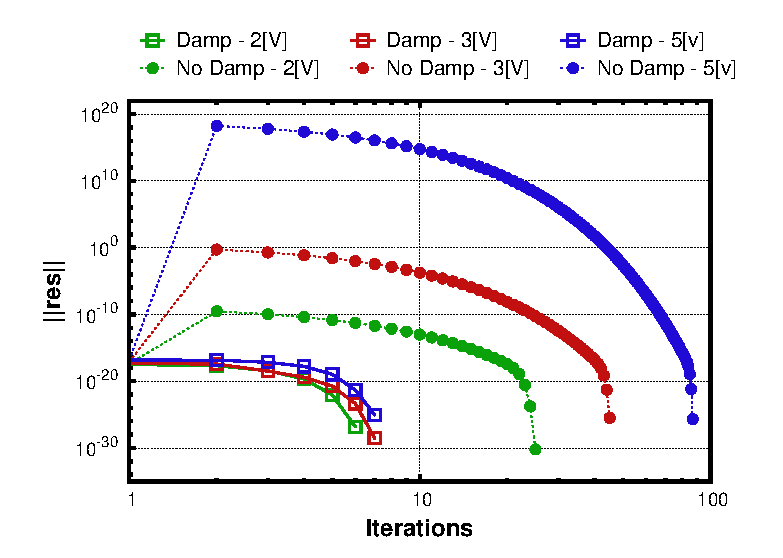
\includegraphics[height=7cm]{FiniteElementDiscretization/NLPconver/NLPconvergence.eps}}

\subfloat[][\emph{$t_k$ parameter.}]
{\includegraphics[height=7cm]{FiniteElementDiscretization/NLPconver/NLPtheta}}

\caption{(a) Number of iteration against residual for different voltages in a diode test case. (b) Magnitude of the damping parameter $t_k$.}

\end{figure}




\subsection{Continuity equations}
\label{sec: continuity equations}

As regards the \referenzaeq{eq: system continuity equation} equation we can write the bilinear form as

\begin{equation}
\label{eq: weak formulation displacement}
a(u,v) =  \int_{\Omega_{Si}}  q D_n e^{(\varphi^{i}/V_{th})} \nabla \psi_j \nabla \psi_i \, d\Omega + \int_{\Omega_{Si}} \sigma_n^{i-1} e^{(\varphi^{i}/V_{th})} \psi_j \psi_i \, d\Omega
\end{equation}

Even if this form guarantees an easily analysis of well-posedness, the choice of using Slotboom variables $u_n$ and $u_p$ causes the onset of overflow problems due to the evaluation of $exp(\varphi/V_{th})$, which can be a rapidly varying function according to the behaviour of the potential $\varphi$.

Therefore special care has to be taken in the treatment of the diffusion coefficient. In view of further discussions of this issue, we introduce some useful notation. For each set $S \subset \Omega$ having measure $|S|$, we introduce the following averages of a given function $g$ that is integrable on $S$:

\begin{equation*}
\mathcal{M}_S(g) = \dfrac{\int_S g \, dS}{|S|} \psp{15} \mathcal{H}_S = (\mathcal{M}_S(g^{-1}))^{-1} 
\end{equation*}

Notice that $\mathcal{M}_S$ is the usual integral average, while $\mathcal{H}_S$ is the \textit{harmonic average}. It is well-known that the use of the harmonic average provides a superior approximation performance \cite{BabuskaMixMet}.


The weak form \referenzaeq{eq: weak formulation displacement}  is the result of a displacement approach which is the most classical way of setting these problems, although different variational formulations and therefore different finite element approximations may be used, like a primal mixed approach (PM) (for a more complete treatment see \cite{Zikatanov:EAFE} and \cite{TesiDotDeFalco}).  First of all it's convenient to reformulate problem \referenzaeq{eq: LEC system new} by using the relation \referenzaeq{eq: un slotboom} and \referenzaeq{eq: Jn slotboom} in a more generic form. This yields the following equivalent form

\begin{equation}
\label{eq: LEC system slotboom generic}
\begin{cases}
\nabla \cdot (\vect{J}_n(n) ) +\sigma n = f & in \psp{3} \Omega_{Si}
 \\
 \vect{J}_n = qD_n e^{(\varphi/V_{th})} \nabla (e^{(-\varphi/V_{th})}n) & in \psp{3} \Omega_{Si}\\
n = n_D & on \psp{3} \Gamma_{D,Si}
 \\
 \vect{J}_n \cdot \vect{n} = 0 & on \psp{3} \Gamma_{N,Si}
\end{cases}
\end{equation}

We report here the weak formulation of \referenzaeq{eq: LEC system slotboom generic} which is well investigated in \cite{TesiDotDeFalco}, find $\vect{J}_n \in [L^2(\Omega)]^d$ and $n \in H^1_{\Gamma_{D,Si}}(\Omega)$ such that

\begin{align}
- \int_{\Omega_{Si}} \vect{J}_n\cdot \nabla v \, d\Omega + \int_{\Omega_{Si}} \sigma n v \, d\Omega = \int_{\Omega_{Si}} f v \, d\Omega \psp{10} \forall v \in H^1_{\Gamma_{D,Si}}(\Omega)
\label{eq: weak form PM1} \\
\int_{\Omega_{Si}} (qD_n e^{(\varphi/V_{th})})^{-1} \vect{J}_n\cdot \vect{q} \, d\Omega + \int_{\Omega_{Si}} \nabla(e^{(\varphi/V_{th})}n) \cdot \vect{q} \, d\Omega = 0 \psp{10} \forall \vect{q} \in [L^2(\Omega)]^d \label{eq: weak form PM2} 
\end{align}

In order to approximate $[L^2(\Omega)]^d$ we introduce a new discrete space

\begin{equation}
\Sigma_h := \left\{   \vect{q}_h \in  [L^2(\Omega)]^d : \vect{q}|_{K} \in [\mathbb{P}_0]^d \forall K \in \mathcal{T}_h\right\}
\end{equation} 

as usual $d$ is the dimension of $\Omega$ and if $d=3$, $\vect{q}_h$ is characterized for every $K \in \mathcal{T}_h$ by the triplet

\begin{equation}
\label{eq: form of qh}
\vect{q}^h_{1,2,3} = \left\{ \begin{bmatrix} 1 \\ 0 \\ 0 \end{bmatrix}  \begin{bmatrix} 0 \\ 1 \\ 0 \end{bmatrix}  \begin{bmatrix} 0 \\ 0 \\ 1 \end{bmatrix}  \right\}
\end{equation}

Therefore \referenzaeq{eq: weak form PM1} and \referenzaeq{eq: weak form PM2} can restricted on a generic element $K$ and the related bilinear form reads

\begin{equation}
\label{eq: LEC discretized general}
\left\{
\begin{array}{rcl}
a_h^K(n_h,v_h) & = & \int_{K}\vect{ J}_{n,h}^K(n_h) \nabla v_h \, dK + \int_{K} \sigma n_h v_h \, dK 
\\
\\
F(v_h)^K & = & \int_K f v_h \, dK
\\
\\
\vect{J}_{n,h}^K & = & D_K(qD_n e^{(\varphi/V_{th})}) \nabla  (e^{(-\varphi / V_{th})}n_h)
\end{array}
\right.
\end{equation}

where $D_K \in \mathbb{R}^{3\times 3}$ is the element stiffness matrix. Several treatments may be performed on this matrix

\begin{equation}
\label{eq: vari diffusion coeff}
 D_K(qD_n e^{(\varphi/V_{th})}) = 
 	\begin{cases}
		  \mathcal{M}_K(qD_n e^{(\varphi/V_{th})}) \\
		  \mathcal{H}_K(qD_n e^{(\varphi/V_{th})}) \\
 		  \dfrac{1}{|K|}\sum_{i=1}^6 \mathcal{H}_{e_i}(qD_ne^{(\varphi/V_{th})}) |e_i| s_i \vect{t}_i \vect{t}_i^T
 		 \end{cases}
\end{equation}


These different approaches in the computation of the average of the diffusion coefficient are responsible for the quite different numerical perfomance of the relative methods.
We already presented the standard average and the armonic average and we discussed briefly the advantages of them. 
The latter equation in \referenzaeq{eq: vari diffusion coeff} introduces an exponentially treatment of the diffusion coefficient along each edge of the boundary $\partial K$ of the subdomain $K$. 

Considering that along the edges the approximate flux density can be written as a function of its tangential components. We have for each edge $e_i$, the tangential component of $J_h^K(n_h)$

\begin{align*}
j_{e_i}  & =   \mathcal{H}_{e_i} \dfrac{\delta_i(e^{-\varphi /V_th}n_h)}{|e_i|} = \mathcal{H}_{e_i} \nabla (e^{-\varphi / V_{th}}n_h) \vect{t}_i \\
& =  \mathcal{H}_{e_i}(qD_n e^{(\varphi/V_{th})}) \dfrac{\mathcal{B}(\delta_i(\varphi / V_{th}))n_{h,k} -  \mathcal{B}(-\delta_i(\varphi / V_{th}))n_{h,j}}{|e_i|}
\end{align*}

where 

\begin{equation}
\label{eq: peclet number}
\delta_i(\varphi / V_{th}) = \dfrac{\varphi_k - \varphi_j}{V_{th}} = 2 \dfrac{(\vect{E}_K\cdot \vect{t}_{e_i}) |e_i|}{2\mathcal{H}_{e_i}(qD_n e^{(\varphi/V_{th})}) } = 2 \gamma_i
\end{equation}

\begin{equation}
\mathcal{B}(z) = \left\{ \begin{array}{cl}
\dfrac{z}{e^z-1} & z \neq 0
\\
1 & z = 0
\end{array}
\right.
\end{equation}

being $\vect{E}_K$ the relative electric field on $K$ and $|\gamma_i|$ the P\`eclet number associated with the edge $e_i$. 
From \referenzaeq{eq: LEC discretized general} we immeditaly obtain:

\begin{equation}
\label{eq: exp fitted flux}
\vect{J}_h^K = \dfrac{1}{|K|}\sum_{i=1}^6 |e_i| s_i j_{e_i} \vect{t}_i 
\end{equation}

Furthermore having defined the flux vector over $K$ in the form \referenzaeq{eq: exp fitted flux}, it is possible to construct a fimily of Galerkin finite element approximations for the continuity equations by a proper choice of the quantities $j_{e_i}$ (e.g. upwind techniques). 




\subsubsection{The discretization scheme}

Given the choice for $j_{e_i}$ and replacing the equation for $\vect{J}_h^K$ in the bilinear form \referenzaeq{eq: LEC discretized general}, we can compute the local system matrix as

\begin{equation}
\Phi_K  = 
{
\tiny 
\left[
\begin{array}{cccc}
- \left( \begin{array}{c}
a_{e12}\mathcal{B}_{12}L^K_{21} + \\
a_{e13}\mathcal{B}_{13}L^K_{31} + \\
a_{e14}\mathcal{B}_{14}L^K_{41}
\end{array} \right)

& a_{e12}\mathcal{B}_{12}L^K_{21} 
& a_{e13}\mathcal{B}_{13}L^K_{31}
& a_{e14}\mathcal{B}_{14}L^K_{41}
\\

%-----------------------------
a_{e21}\mathcal{B}_{21}L^K_{12}
&
- \left( \begin{array}{c}
a_{e21}\mathcal{B}_{21}L^K_{12} + \\
a_{e23}\mathcal{B}_{23}L^K_{32} + \\
a_{e24}\mathcal{B}_{24}L^K_{42}
\end{array} \right)
& a_{e23}\mathcal{B}_{12}L^K_{32}
& a_{e24}\mathcal{B}_{12}L^K_{42}
\\

%-----------------------------
a_{e31}\mathcal{B}_{31}L^K_{31}
& a_{e31}\mathcal{B}_{32}L^K_{32}
&
- \left( \begin{array}{c}
a_{e31}\mathcal{B}_{31}L^K_{31} + \\
a_{e32}\mathcal{B}_{32}L^K_{32} + \\
a_{e34}\mathcal{B}_{34}L^K_{34}
\end{array} \right)

&a_{e34}\mathcal{B}_{34}L^K_{34}
\\

%-----------------------------
a_{e41}\mathcal{B}_{41}L^K_{41}
& a_{e42}\mathcal{B}_{42}L^K_{42}
&a_{e43}\mathcal{B}_{43}L^K_{43}
&
- \left( \begin{array}{c}
a_{e41}\mathcal{B}_{41}L^K_{41} + \\
a_{e42}\mathcal{B}_{42}L^K_{42} + \\
a_{e43}\mathcal{B}_{43}L^K_{43}
\end{array} \right)

\end{array}
\right]
}
\end{equation}

\begin{equation}
\label{eq: matrice continuità}
A_K = \Phi_K + \dfrac{|K|}{4} diag (\sigma)
\end{equation}

\begin{equation}
\vect{F}_K = \dfrac{|K|}{4} (f_1,f_2,f_3,f_4)^T
\end{equation}

denoting by  $\mathcal{B}_{ij}$ the Bernoulli function applied to the potential difference between node $j$ and node $i$.

The discretization scheme just presented is well known as \textit{Edge Averaged Finite Elements} (EAFE) and it's particularly suitable for problems with  highly variable coefficient. Furthermore this approach has several good properties, e.i. in 2D simulation if $\mathcal{T}_h$ is a Delauny partition the system matrix is an \textit{M-matrix} \cite{BankMmatrixEAFE}. The main consequence of this statement is that the solution could satisfy the \textit{Discrete Maximum Principle}. This is a notable property which implies that no negative concentrations are admitted. Unfortunately this property is not anymore valid in 3D framework, indeed the Delauny condition of the mesh is not sufficient to guarantee that the system matrix is an M-matrix. A more general condition is presented in \cite{ZikatanovXu}.

\begin{Teorema}[Zikatanov condition]
The system matrix of the EAFE scheme is an M-matrix if and only if for any fixed edge E of the partition $\mathcal{T}_h$ the following inequality holds:

\begin{equation}
\label{eq: mesh delaunay condition}
\omega_E = \dfrac{1}{n(n-1)} \sum_{T\supset E} |k_E^T|cot\theta_E^T \geq 0,
\end{equation}

where $n$ is the dimension, $\sum_{T \supset E}$ means summation over all simplexes $T$ containing $E$, $\theta_E^T$ is tha angle between the faces $f_i$, $f_j \in \mathcal{T}_h$ such that $f_i \bigcap f_j = E$  and $k_E^T$ is the edge in $T$ which doesn't share any verticies with $E$.
\end{Teorema}

\begin{Osservazione}
For $n=2$ the condition \referenzaeq{eq: mesh delaunay condition} means that the sum of the angles opposite to any edge is less than or equal to $\pi$, this condition implies that the partition is a Delaunay triangulation.
\end{Osservazione}

\begin{Osservazione}
Condition \referenzaeq{eq: mesh delaunay condition} highlights that in order to satisfy the discrete maximum principle, a partion without obtuse angles is preferable.
\end{Osservazione}

We remark that presently meshing algorithm are oriented to care about the minimum angle of the elements, rather than the maximum, resulting that obtain a mesh which satisfied the condition \referenzaeq{eq: mesh delaunay condition} it's a really difficult task. 

\figref{fig: cubo zikatanov} shows a simple partition of a cube performed with the Synopsis tool SNMESH. For every element we evaluated how many edges don't satisfy the condition \referenzaeq{eq: mesh delaunay condition}.
It's clear that there are a lot of edges which don't fulfill the condition and a precise pattern can't be individuated. When several bad edges belong to a single element we can indentify the presence of many obtuse angles.

In order to avoid this problem some alternative solutions are proposed in the literature, like the \textit{Orthogonal Subdomain Collocation method} \cite{OSCputticorded}, but also this approach is not definitely. 

Therefore in presence of negative concentration the most used technique during 3D numerical simulation is the increasing of the degree of freedom in the problematic regions, which often are the ones where the carrier density decrease.



\begin{figure}[!b]
\centering
{\includegraphics[width=0.75\textwidth , height = 5.5cm]{FiniteElementDiscretization/CuboElementi.png}}
\caption{Evaluation of the Zikatanov condition over a simple partition. Red elements doesn't satisfy condition  \referenzaeq{eq: mesh delaunay condition} over four edges while blue elements fully accomplished the criterion.}
\label{fig: cubo zikatanov}
\end{figure}

%\textcolor{red}{Vale la seguente uguaglianza?}
%\begin{equation}
%L_{ij} = s_{ij} \vect{t}_{ij} \cdot \nabla \psi_i
%\end{equation}
\clearpage
\chapter{Simulation results}

In this chapter we present the results obtained to validate the numerical performance of the discretization method described in the previously chapters, compared with a reference simulation tool (SDEVICE \textcolor{red}{ref}). Moreover we describe (and compare) the algorithm used to calculate the current at contacts.

\section{Test cases}

We consider three kind of semiconductor devices: 

\begin{itemize}
\item {\bf p-n junction}
\item {\bf p-n junction in oxide}
\item {\bf MOSFET n-channel / p-channel}
\end{itemize}

\subsection{p-n junction}
\label{sec: PN}

In this example we consider a simple p-n junction. \figref{fig: diodo struttura} presents the partition used and the doping profile of this test case. The section of the parallelepiped is a $0.05 \times 0.05 [\mu m^2]$ square while the device is $0.1 [\mu m]$ long.  The number of verticises are $4933$, while the elements are $24576$.  The doping concentration is obtained setting a constant profile of acceptors over all the domain ($N_A = 1.0\times 10^{17}$) overhelmed by a doping profile of  donors ($N_D=1.0 \times 10^{18}$) bounded on one side of the device resulting in an almost abrupt junction. 
Two contacts are defined: (A) contact is placed at $Z=0.1[\mu m]$ and (B) contact is placed at $Z=0.0 [\mu m]$.  


\begin{figure}[!t]
\centering
\subfloat[][\emph{Mesh}]
{\includegraphics[height=3.5cm]{Results/DIODE/AAA_structureandcontactFINITO.png}}
\hspace{1cm}
\subfloat[][\emph{Doping concentration}]
{\includegraphics[height=3.5cm]{Results/DIODE/AAADopingConcentrationFINITO.png}}
\label{fig: diodo struttura}
\end{figure}


We proceed in order to analyze the operating function of the diode, therefore two cases in direct polarization are performed. The setting values and the parameters are summerized in \ref{tab: diode direct}. 




\figref{fig: Solutions case test 0.3} and \figref{fig: Solutions case diode 1V} report the behaviour of the solutions along a line parallel to the Z-axis and placed at the center of the device. 

Because the built-in voltage is around $0.7 \div 0.8 [V]$ the behaviour of the device is different when the applied bias is below or above the built-in voltage. 
At $0.3[V]$ of polarization potential drop is almost bounded around the junction, and due to the asymmetric doping, is major extended in the p-side. The carriers can't easily cross the potential barrier and this will cause a low current flux inside the device.
At $1.0[V]$ the minority carriers density becomes almost ten order bigger, resulting in a large ammount of current toward the contacts:  the device turns from exponential to linear resistive. This is clear in \figref{fig: diode 1v pot} where the potential shape becomes similar to a resistence voltage profile.  

Comparing the quasi-fermi potential of \figref{fig: qf pot diode 03} and \figref{fig: qf pot diode 1} the boundary layers at contacts increase with the polarization. This effect is related to the ohmic contact hypotesis, and can be avoided with different boundary condition, this occurs also for the carrier concentration because at the contacts the charge neutrality and the thermodynamic equilibrium  are imposed.

\figref{fig: diode potential 03V}$\div$\ref{fig: pdensity 03V} shows the comparison between SDEVICE and FEMOS in 3D plots for electrostatic potential, electron and hole densities for bias at $0.3[V]$, while \figref{fig: diode potential 1V}$\div$\ref{fig: pdensity 1V} show the shape comparison for bias at $1.0[V]$. In both of the condition the agreement is very good.


\begin{figure}[!h]
\centering

\subfloat[][\emph{Potential}]
{\includegraphics[height=4.5cm]{DatiImmaginiTESI/Diode/PotentialZaxis03volt.eps}}
\subfloat[][\emph{Potential} \label{fig: diode 1v pot}]
{\includegraphics[height=4.5cm]{DatiImmaginiTESI/Diode/PotentialZaxis1volt.eps}}


\subfloat[][\emph{Carriers}]
{\includegraphics[height=4.5cm]{DatiImmaginiTESI/Diode/DensitiesZaxis03volt.eps}}
\subfloat[][\emph{Carriers}]
{\includegraphics[height=4.5cm]{DatiImmaginiTESI/Diode/DensitiesZaxis1volt.eps}}


\subfloat[][\emph{Quasi fermi potential} \label{fig: qf pot diode 03}]
{\includegraphics[height=4.5cm]{DatiImmaginiTESI/Diode/QuasiFermiZaxis03volt.eps}}
\subfloat[][\emph{Quasi fermi potential} \label{fig: qf pot diode 1}]
{\includegraphics[height=4.5cm]{DatiImmaginiTESI/Diode/QuasiFermiZaxis1volt.eps}}

\caption{Solutions case test diode $V=0.3[V]$.}
\label{fig: Solutions case test 0.3}
\end{figure}

\begin{table}[!h]
\centering
\begin{tabular}{ccccc}
\toprule
 Test case & Mobility model & R/G model & $\epsilon_{Si}$ & $\epsilon_{0x}$  \\
\midrule
$V_A=0.3 [V]$ & $\mu_n = 1417$, $\mu_p = 470.5$ & SRH, Auger & 11.6 & - \\
$V_A=1.0 [V]$ & $\mu_n = 1417$, $\mu_p = 470.5$ & SRH, Auger & 11.6 & - \\\bottomrule
\end{tabular}
\caption{p-n junction - list of parameters.}
\label{tab: diode direct}
\end{table}



\clearpage 

\begin{figure}[!h]
\centering
\subfloat[][\emph{FEMOS}]
{\includegraphics[height=3.7cm]{Results/DIODE/FEMOS1817_potential03volt.png}}
\hspace{1cm}
\subfloat[][\emph{SDEVICE}]
{\includegraphics[height=3.7cm]{Results/DIODE/SDEVICE1817_potential03voltONLYDEVICE.png}}
\caption{p-n junction 0.3[V] - Potential.}
\label{fig: diode potential 03V}
\end{figure}

\vspace{1cm}

\begin{figure}[!h]
\centering
\subfloat[][\emph{FEMOS}]
{\includegraphics[height=3.7cm]{Results/DIODE/FEMOS1817_edensity03volt.png}}
\hspace{1cm}
\subfloat[][\emph{SDEVICE}]
{\includegraphics[height=3.7cm]{Results/DIODE/SDEVICE1817_edensity03voltONLYDEVICE.png}}
\caption{p-n junction 0.3[V] -  Electron density.}
\label{fig: ndensity 03V}
\end{figure}

\vspace{1cm}

\begin{figure}[!h]
\centering
\subfloat[][\emph{FEMOS}]
{\includegraphics[height=3.7cm]{Results/DIODE/FEMOS1817_hdensity03volt.png}}
\hspace{1cm}
\subfloat[][\emph{SDEVICE}]
{\includegraphics[height=3.7cm]{Results/DIODE/SDEVICE1817_hdensity03voltONLYDEVICE.png}}
\caption{p-n junction 0.3[V] - Hole density.}
\label{fig: pdensity 03V}
\end{figure}


\clearpage

\begin{figure}[!h]
\centering
\subfloat[][\emph{FEMOS}]
{\includegraphics[height=3.7cm]{Results/DIODE/FEMOS1817_potential1voltONLYDEVICE.png}}
\hspace{0.7cm}
\subfloat[][\emph{SDEVICE}]
{\includegraphics[height=3.7cm]{Results/DIODE/SDEVICE1817_potential1volt.png}}
\caption{p-n junction 1.0[V] - Potential.}
\label{fig: diode potential 1V}
\end{figure}

\vspace{1cm}

\begin{figure}[!h]
\centering
\subfloat[][\emph{FEMOS}]
{\includegraphics[height=3.7cm]{Results/DIODE/FEMOS1817_edensity1voltLINEARONLYDEVICE.png}}
\hspace{0.7cm}
\subfloat[][\emph{SDEVICE}]
{\includegraphics[height=3.7cm]{Results/DIODE/SDEVICE1817_edensity1voltLINEARWITHLEGEND.png}}
\caption{p-n junction 1.0[V] -  Electron density.}
\label{fig: ndensity 1V}
\end{figure}

\vspace{1cm}

\begin{figure}[!h]
\centering
\subfloat[][\emph{FEMOS}]
{\includegraphics[height=3.7cm]{Results/DIODE/FEMOS1817_hdensity1voltLINEARONLYDEVICE.png}}
\hspace{0.7cm}
\subfloat[][\emph{SDEVICE}]
{\includegraphics[height=3.7cm]{Results/DIODE/SDEVICE1817_hdensity1voltLINEARWITHLEGEND.png}}
\caption{p-n junction 1.0[V] - Hole density.}
\label{fig: pdensity 1V}
\end{figure}

\clearpage

\subsubsection{Computational cost and initial condition}

It's well known that the convergence time is strictly related to the kind of initial condition on device. However predict in every situations the possibly shape of the solutions is hard, if not even impossible. For this reason we have adopted a common and general approach splitting the domain in several regions accordingly to their doping concentration: each of the semiconductor regions are treated as they are in equilibrium with the nearest contact then the guess value for $\varphi$ is obtained thanks to the relations \referenzaeq{eq: non eq n density mb} or \referenzaeq{eq: non eq p density mb}. 

It's quite simple implement this kind of initial profile and it's reasonable thinking that for solutions near the equilibrium this method will guarantee good converging performances. 

In order to analyze the response of the system at different bias an additional case test is proposed. In the range between $0.0[V]$ and $3.0[V]$ several voltages were applied on the previous device. For every bias point the initial guess is computed with the above mentioned way. 

\figref{fig: tempi computazionali 1} shows how the computational cost of computing the solution increases with the increasing of the applied bias. Moreover as expected if the mesh is finer the time needed to find the solution increases, resulting in a rigid shift of the curve toward high time value.


\begin{figure}[!b]
\centering
\includegraphics[height=7cm]
{Results/Caratteristiche/Diode/ComputationalTimeDifferentMeshes.eps}
\caption{Total time Gummel Map.}
 \label{fig: tempi computazionali 1}
 \end{figure}
 
 
Focusing on the case test related to the coarser mesh additional considerations may be done. In \figref{fig: tempi computazionali 2} it's evident how the average time spent to solve the NLP and the DD equations remains almost unchanged. On the contrary the number of GM iterations needed by the system to reach the solution, increases for voltages above $1.5[V]$.

A reasonable explanation of this phenomenon could be found comparing solution and initial guess for a bias below and above $1.5[V]$ (similar considerations may be done if we consider the carrier densities). When voltage is low, like in \figref{fig: different biast initial step 1} ($V_A = 0.1[V]$), the potential shape is well predicted by the initial guess, resulting easier for the Gummel map converging toward the solution. On the contrary in \figref{fig: different biast initial step 2} ($V_A=1.6[V]$) the device operates as a resistence and the potential profile seems more to a linear function, this implies that from an initial condition of equilibrium the algorithm have to spent more steps in order to reach the solution. 


 
 \begin{figure}[!t]
\centering
\includegraphics[height=7cm]{Results/Caratteristiche/Diode/ConfrontoTempiNLPDDGMiterations.eps}
\caption{Time NLP and DD, iteration GM.}
\label{fig: tempi computazionali 2}
\end{figure}

\begin{figure}[!b]
\centering
\subfloat[][\label{fig: different biast initial step 1}]
{\includegraphics[height=4.5cm]{DatiImmaginiTESI/Diode/PotentialZaxis01volt.eps}}
\subfloat[][\label{fig: different biast initial step 2}]
{\includegraphics[height=4.5cm]{DatiImmaginiTESI/Diode/PotentialZaxis15volt.eps}}
\caption{Initial step for different bias.}
\label{fig: different biast initial step}
\end{figure}
 



\clearpage


\subsection{p-n junction in oxide}
\label{sec: PNOX}

In this test case a silicon p-n junction of $0.3[\mu m]$ long has been surrounded by an oxide layer of $0.025[\mu m]$ thick. The section of the slicon part is a $0.1 \times 0.1 [\mu m^2]$ square.  We spent $6334$ verticies overall the domain \textcolor{red}{elements}. The structure and the doping are well defined in \figref{fig: structure diodeox}. The setting of the electrode is similar to the previously test case and contacts are defined only on silicon surface. 
\tabref{tab: diodeox 3d} reports the models and parameters used.

\figref{fig: plot 1D diodeox} reports the behaviour of the solutions and the quasi fermi potential levels along a line parallel to the Z-axis and placed at the center of the device. The main features are similar to the previous device, indeed notice the boundary layers at contact for the carrier densities and the quasi fermi potential levels.
\figref{fig: potential diodeox} $\div$ \ref{fig: hdensity diodeox} show the 3D solutions for the case at $0.3[V]$, while \figref{fig: potential diodeox 1V}$\div$\ref{fig: hdensity diodeox 1V} refer to the case at $1.0[V]$. Both in 1D and 3D comparison charts the agreement with the commercial software is good. 

\vspace{0.5cm}

\begin{figure}[!h]
\centering
\subfloat[][\emph{Mesh}]
{\includegraphics[height=4.5cm]{Results/DIODEOX/AAA_structureandcontact2.png}}
\hspace{1.5cm}
\subfloat[][\emph{Doping concentration}]
{\includegraphics[height=4.5cm]{Results/DIODEOX/AAA_Dopingconcentration2ONLYDEVICE.png}}
\caption{Test case p-n junction in oxide.}
\label{fig: structure diodeox}
\end{figure}


\vspace{0.5cm}

\begin{table}[!h]
\centering
\begin{tabular}{ccccc}
\toprule
 Test case & Mobility model & R/G model & $\epsilon_{Si}$ & $\epsilon_{0x}$  \\
\midrule
$V_A=0.3 [V]$ & $\mu_n = 1417$, $\mu_p = 470.5$ & SRH, Auger & 11.6 & 3.9 \\
$V_A=1.0 [V]$ & $\mu_n = 1417$, $\mu_p = 470.5$ & SRH, Auger & 11.6 & 3.9 \\\bottomrule
\end{tabular}
\caption{List of parameters.}
\label{tab: diodeox 3d}
\end{table}




\begin{figure}[!t]
\centering

\subfloat[][\emph{Electrostatic potential.}]
{\includegraphics[height=4.6cm]{DatiImmaginiTESI/DiodeOx/PotentialZaxis.eps}}
\subfloat[][\emph{Electrostatic potential.}]
{\includegraphics[height=4.6cm]{DatiImmaginiTESI/DiodeOx/PotentialZaxis1VOLT.eps}}


\subfloat[][\emph{Hole and electron densities.}]
{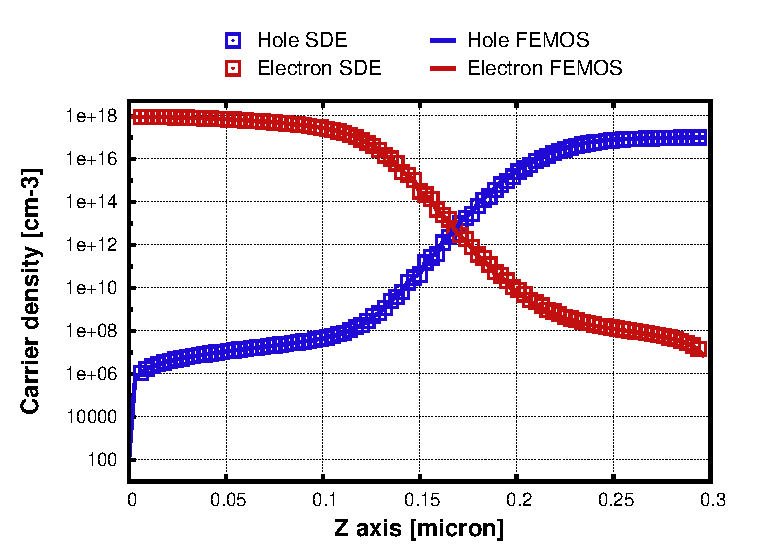
\includegraphics[height=4.6cm]{DatiImmaginiTESI/DiodeOx/DensityZaxis.eps}}
\subfloat[][\emph{Hole and electron densities.}]
{\includegraphics[height=4.6cm]{DatiImmaginiTESI/DiodeOx/DensityZaxis1VOLT.eps}}


\subfloat[][\emph{Quasi fermi potential levels.}]
{\includegraphics[height=4.6cm]{DatiImmaginiTESI/DiodeOx/QFPotentialZaxis.eps}}
\subfloat[][\emph{Quasi fermi potential levels.}]
{\includegraphics[height=4.6cm]{DatiImmaginiTESI/DiodeOx/QFPotentialZaxis1VOLT.eps}}


\caption{Plots of the solutions and the quasi fermi potential levels along the line parallel to the Z-axis and placed at the center of the device. On the left is presented the test case at $V_a=0.3[V]$ while on the left at $V_A=1.0[V]$.}
\label{fig: plot 1D diodeox}
\end{figure}

\clearpage


\begin{figure}[!h]
\centering
\subfloat[][\emph{FEMOS}]
{\includegraphics[height=4.5cm]{Results/DIODEOX/FEMOS1817_potential03volt.png}}
\hspace{1cm}
\subfloat[][\emph{SDEVICE}]
{\includegraphics[height=4.5cm]{Results/DIODEOX/SDEVICE1817_potential03voltONLYDEVICE.png}}
\caption{p-n junction in oxide 0.3[V] - Potential.}
\label{fig: potential diodeox}
\end{figure}

\vspace{0.5cm}

\begin{figure}[!h]
\centering
\subfloat[][\emph{FEMOS}]
{\includegraphics[height=4.5cm]{Results/DIODEOX/FEMOS1817_edensity03volt.png}}
\hspace{1cm}
\subfloat[][\emph{SDEVICE}]
{\includegraphics[height=4.5cm]{Results/DIODEOX/SDEVICE1817_edensity03voltONLYDEVICE.png}}
\caption{p-n junction in oxide 0.3[V] - Electron density.}
\label{fig: edensity diodeox}
\end{figure}

\vspace{0.5cm}

\begin{figure}[!h]
\centering
\subfloat[][\emph{FEMOS}]
{\includegraphics[height=4.5cm]{Results/DIODEOX/FEMOS1817_hdensity03volt.png}}
\hspace{1cm}
\subfloat[][\emph{SDEVICE}]
{\includegraphics[height=4.5cm]{Results/DIODEOX/SDEVICE1817_hdensity03voltONLYDEVICE.png}}
\caption{p-n junction in oxide 0.3[V] - Hole density.}
\label{fig: hdensity diodeox}
\end{figure}

\clearpage


\begin{figure}[!h]
\centering
\subfloat[][\emph{FEMOS}]
{\includegraphics[height=4.5cm]{Results/DIODEOX/FEMOS1817_potential1voltONLYDEVICE.png}}
\hspace{1cm}
\subfloat[][\emph{SDEVICE}]
{\includegraphics[height=4.5cm]{Results/DIODEOX/SDEVICE1817_potential1voltONLYDEVICE.png}}
\caption{p-n junction in oxide 1.0[V] - Potential.}
\label{fig: potential diodeox 1V}
\end{figure}

\vspace{0.5cm}

\begin{figure}[!h]
\centering
\subfloat[][\emph{FEMOS}]
{\includegraphics[height=4.5cm]{Results/DIODEOX/EdensityLINEARDIODEOXONLYDEVICE.png}}
\hspace{1cm}
\subfloat[][\emph{SDEVICE}]
{\includegraphics[height=4.5cm]{Results/DIODEOX/EdensityLINEARDIODEOXONLYDEVICEsde.png}}
\caption{p-n junction in oxide 1.0[V] - Electron density.}
\label{fig: edensity diodeox 1V}
\end{figure}

\vspace{0.5cm}

\begin{figure}[!h]
\centering
\subfloat[][\emph{FEMOS}]
{\includegraphics[height=4.5cm]{Results/DIODEOX/HdensityLINEARDIODEOXONLYDEVICE.png}}
\hspace{1cm}
\subfloat[][\emph{SDEVICE}]
{\includegraphics[height=4.5cm]{Results/DIODEOX/HdensityLINEARDIODEOXONLYDEVICEsde.png}}
\caption{p-n junction in oxide 1.0[V] - Hole density.}
\label{fig: hdensity diodeox 1V}
\end{figure}

\clearpage





\subsubsection{3D effect of the electric field}


Looking at \figref{fig: potential diodeox} it's clear that for low bias the electrostatic potential behaves differently in the two materials.
This phenomena could be explained if we think about the relation \referenzaeq{eq: relazione pot electric} between electric field and potential.
In fact, as we imposed $\nabla \varphi \cdot \vect{n}=0$ on the oxide boundary no field lines of the electric field could cross that boundary. The consequence is that all the field lines could start and end only from the contact A or B.
Polarization can't operate directly on the oxide and the behaviour of the the electric field inside the device is due only to the displacement effect in the junction of the silicon, which imposes the electric response in the oxide material. \figref{fig: electric field diode} reports the field lines of the electric field in the case $V_A=0.3[V]$ comparing with the commercial software. The visible effect is a lower magnitude of the electric field in the oxide, resulting a more diffused potential.

This phenomena seems to disappear for high bias: in \figref{fig: potential diodeox 1V} the influence of the contact (A) becomes much higher and the electorstatic potential tends to conform over the entire domain.



\begin{figure}[!h]
\centering
\subfloat[][\emph{FEMOS}]
{\includegraphics[height=4.7cm]{Results/DIODEOX/FEMOS1817_electricfield03volt.png}}
\hspace{1.5cm}
\subfloat[][\emph{SDEVICE}]
{\includegraphics[height=4.7cm]{Results/DIODEOX/SDEVICE1817_electricfield03voltONLYDEVICE.png}}
\caption{Test case dide p-n in ox 0.3[V], electric field.}
\label{fig: electric field diode}
\end{figure}






It is important to note that displacment approach doesn't satisfied  in a strong manner the pricinple of action and reaction.
This is equivalent to say that given two element $K_i,K_j\in \mathcal{T}_h$ such that $K_i \bigcap K_j = f_i$ where $f_i \in \mathcal{F}_h$ and let be  $\vect{n}_{i}$ the outward normal vector of $\partial K_i$ and $\vect{n}_{j}$ the outward normal vector of $\partial K_j$,  we ensure the following equations only in a weak way

\begin{align}
\vect{D}|_{K_i}\cdot \vect{n}_{i} & = \vect{D}|_{K_j} \cdot \vect{n}_{j} \label{eq: conservazione vettore spostamento}\\
\vect{J}_n|_{K_i}\cdot \vect{n}_{i} & = \vect{J}_n|_{K_j}\cdot \vect{n}_{j} \\
\vect{J}_p|_{K_i}\cdot \vect{n}_{i} & = \vect{J}_p|_{K_j}\cdot \vect{n}_{j} 
\end{align}


In fact taking in consideration equation \referenzaeq{eq: conservazione vettore spostamento}, we can state that along the interface silicon-oxide the following equality holds

\begin{equation}
\epsilon_{ox}\vect{E}|_{K_i}\cdot \vect{n}_{i} = \epsilon_{Si}\vect{E}|_{K_j} \cdot \vect{n}_{j} \psp{5} \Rightarrow \psp{5}  [\vect{E}|_{K_i}]_y = \dfrac{\epsilon_{Si}}{\epsilon_{ox}}[\vect{E}|_{K_j}]_y
\end{equation}  

Accordingly with the parameters used during the simulations $\epsilon_{Si}/\epsilon_{ox}=2.97$, which means that the normal component on the interface of the electric field has a gap passing from oxide to semicondctor and vice versa. \figref{fig: salto electric field} shows a plots of $E_y$ along a line parallel to the Y-axis which crosses both oxide and silicon material. For this setting $E_y\equiv\vect{E}\cdot \vect{n}$ on the interface and the drop of magnitude is quite visible. The ratio between the two interfaces is almost $3.8$ for both $y=0.05[\mu m]$ and $y = 0.15[\mu m]$.
This example really shows the effect of the phenomena we mentionend before and the consequence which the solutions could own.

 Furthermore every tetrahedral interfaces of the partition are affected by this problem, which means that inside an omogenous material the normal component of the electric field doesn't conserve from one element of the grid to the neighbouring ones. Even the presence of this drawback, the solutions obtained are good, but if you would satisfy equation \referenzaeq{eq: conservazione vettore spostamento} in a strong manner you need to move for mixed-hibryd formulation \textcolor{red}{ref} which ensures the conservation of the flux even under possbile strong discontinuities of material properties.


\begin{figure}[!h]
\centering
\includegraphics[height=5cm]{DatiImmaginiTESI/DiodeOx/ElectricFieldYaxis.eps}
\caption{$E_y$ along a line parallel to Y-axis, $z=0.22[\mu m]$ and $x=0.1[\mu m]$.}
\label{fig: salto electric field}
\end{figure}


\clearpage





\subsection{MOSFET n-channel}
\label{sec: MOS}


The description of MOSFET device can be found in \cite{ModernVLSIdevices}: it is a four-terminal device with the electrodes designeted as gate (G), source (S), drain (D) and substrate or bulk (B). The gate electrode is usually made of metal or heavily doped polysilicon and is separated from the substrate by a thin silicon dioxide. The surface region under the gate  oxide between source and drain is called the \textit{channel} region.
Because the current in a MOSFET is transported predominantly by carriers of one polarity, the MOSFET is usually referred to as a unipolar or majority-carrier device, as a propose of test we consider a n-channel (n-MOSFET) or a p-channel (p-MOSFET). An \textit{n-MOSFET} (p-MOSFET) consists of a p-type (n-type) silicon substrate into which two n-regions (p-regions) are the designing source and drain. The n-regions (p-regions) are doped accordingly with a gaussain profile as occuring from an implantation. 
\figref{fig: mos geometry 1} and \figref{fig: mos geometry 2} shows the geometry and the doping concentration for n-MOSFET and p-MOSFET respectively. 
We note that the mesh has been refined where the more interesting phenomena occur: along channel and over the deplation regions.

When no voltage is applied to the gate, no current flows between the source and drain, while if a sufficiently large positive voltage is applied to the gate, the silicon surface is inverted to n-type (p-type), which forms a conducting channel between the source and drain: applying a positive voltage to the drain (source) the electrons (holes) start to flow from source to drain and therefore a current is generated. 

\begin{figure}[!b]
\centering
\subfloat[][\emph{Mesh}\label{fig: mos geometry 1}]
{\includegraphics[height=4.2cm]{Results/MOS/AAA_MeshAndContact.png}}
\hspace{0.5cm}
\subfloat[][\emph{Doping concentration}\label{fig: mos geometry 2}]
{\includegraphics[height=4.2cm]{Results/MOS/AAA_DopingConcentrationONLYDEVICE.png}}
\caption{Geometry of the test case MOS n-channel.}
\label{fig: mos geometry}
\end{figure}




The explanation of the MOSFET working principle has ben clarified in \figref{fig: energy levels MOS} where for the case of n-channel the band profile along the channel axis has been reported for two different gate bias.
The voltage applyed to the gate tends to decrease the flow of the electron as the energy barrier doesn't exist anymore.
\figref{fig: channel figures 1D} shows for an n-channel the profile of carrier concentrations in the middle of the channel cut perpendicular to the gate, for off-state and on-state: the inversion occurs when the gate voltage is higher than MOSFET threshold.
The voltage applyed to the gate tends to decrease the band levels in the channel region: in this configuration the drain voltage causes the flow of the electron as the energy barrier doesn't exist anymore (see \figref{fig: energy levels MOS}).
\figref{fig: channel figures 3D} shows the 3D view of the n-channel space charge after inversion.



\begin{figure}[!t]
\centering
\subfloat[][\emph{$V_G=0.0[V]$, $V_D=0.1[V]$}]
{\includegraphics[scale=0.55]{DatiImmaginiTESI/Mos/BandDiagramMOS0volt.eps}}
\subfloat[][\emph{$V_G=2.0[V]$, $V_D=0.1[V]$}]
{\includegraphics[scale=0.55]{DatiImmaginiTESI/Mos/BandDiagramMOS2volt.eps}}
\caption{Energy band levels.}
\label{fig: energy levels MOS}
\end{figure}



The parameters and models used for these simulations are summerized in \tabref{tab: mos direct pol}. \figref{fig: potential mos off}$\div$\ref{fig: pdensity mos off} shows the 3D components of the electrostatic potential, electron density and hole density between the FEMOS results and the commercial code for the off-state MOSFET, while \figref{fig: potential mos}$\div$\ref{fig: pdensity mos} for the on-state MOSFET: the agreement is very good.


\begin{figure}[!b]
\centering
\subfloat[][1D cut perpendicular to the channel. \label{fig: channel figures 1D}]
{\includegraphics[height=4.5cm]{DatiImmaginiTESI/Mos/DensityZaxis.eps}}
\hspace{1cm}
\subfloat[][Space charge.\label{fig: channel figures 3D}]
{\includegraphics[height=4.5cm]{Results/PlotOverLine/Mos/Contour3DSpacechargeONLYDEVICE}}
\caption{Channel formation of the nMOSFET.}
\label{fig: channel figures}
\end{figure}


Finally \figref{fig: electric field mos} reports the streamline plot of the electric field inside the device for FEMOS and the SDEVICE:
\textcolor{red}{????}

\begin{figure}[!h]
\centering
\subfloat[][\emph{FEMOS}]
{\includegraphics[height=4.5cm]{Results/MOS/FEMOS181718_ElectricField2voltONLYDEVICE.png}}
\hspace{0.5cm}
\subfloat[][\emph{SDEVICE}]
{\includegraphics[height=4.5cm]{Results/MOS/SDEVICE181718_ElectricField2voltONLYDEVICE.png}}
\caption{Electric field density - $V_G = 2.0 [V]$.}
\label{fig: electric field mos}
\end{figure}

\vspace{0.5cm}



\begin{table}[!h]
\centering
\begin{tabular}{ccccc}
\toprule
 Test case & Mobility model & R/G model & $\epsilon_{Si}$ & $\epsilon_{0x}$  \\
\midrule
 $V_G=0.0 [V]$, $V_D=0.0[V]$,& $\mu_n = 1417$ & \multirow{2}*{SRH, Auger, II} & \multirow{2}*{11.6} & \multirow{2}*{3.9} \\
 $V_S=V_B=0.0[V]$ & $\mu_p = 470.5$ & & & \\ 
\midrule
$V_G=2.0 [V]$, $V_D=0.1[V]$,& $\mu_n = 1417$ & \multirow{2}*{SRH, Auger} & \multirow{2}*{11.6} & \multirow{2}*{3.9} \\
 $V_S=V_B=0.0[V]$ & $\mu_p = 470.5$ & & & \\
 \bottomrule
\end{tabular}
\caption{List of parameters.}
\label{tab: mos direct pol}
\end{table}

\clearpage

\begin{figure}[!h]
\centering
\subfloat[][\emph{FEMOS}]
{\includegraphics[height=4.4cm]{Results/MOS/MOSNelectrostaticpotSUBTHRESONLYDEVICE.png}}
\hspace{0.8cm}
\subfloat[][\emph{SDEVICE}]
{\includegraphics[height=4.4cm]{Results/MOS/MOSNelectrostaticpotSUBTHRESwithlegend.png}}
\caption{Electrostatic potential - $V_G = 0.0 [V]$.}
\label{fig: potential mos off}
\end{figure}

\vspace{0.5cm}

\begin{figure}[!h]
\centering
\subfloat[][\emph{FEMOS}]
{\includegraphics[height=4.4cm]{Results/MOS/MOSNedensitySUBTHRESONLYDEVICE.png}}
\hspace{0.8cm}
\subfloat[][\emph{SDEVICE}]
{\includegraphics[height=4.4cm]{Results/MOS/MOSNedensitySUBTHRESwithlegend.png}}
\caption{Electron density - $V_G = 0.0 [V]$.}
\label{fig: ndensity mos off}
\end{figure}

\vspace{0.5cm}

\begin{figure}[!h]
\centering
\subfloat[][\emph{FEMOS}]
{\includegraphics[height=4.4cm]{Results/MOS/MOSNhdensitySUBTHRESONLYDEVICE.png}}
\hspace{0.8cm}
\subfloat[][\emph{SDEVICE}]
{\includegraphics[height=4.4cm]{Results/MOS/MOSNhdensitySUBTHRESwithlegend.png}}
\caption{Electron density - $V_G = 0.0 [V]$.}
\label{fig: pdensity mos off}
\end{figure}






\clearpage

\begin{figure}[!h]
\centering
\subfloat[][\emph{FEMOS}]
{\includegraphics[height=4.5cm]{Results/MOS/FEMOS181718_potential2voltONLYDEVICE.png}}
\hspace{0.8cm}
\subfloat[][\emph{SDEVICE}]
{\includegraphics[height=4.5cm]{Results/MOS/SDEVICE181718_potential2voltONLYDEVICE.png}}
\caption{Electrostatic potential - $V_G = 2.0 [V]$.}
\label{fig: potential mos}
\end{figure}

\vspace{0.5cm}

\begin{figure}[!h]
\centering
\subfloat[][\emph{FEMOS}]
{\includegraphics[height=4.5cm]{Results/MOS/FEMOS181718_ndensity2voltONLYDEVICE.png}}
\hspace{0.8cm}
\subfloat[][\emph{SDEVICE}]
{\includegraphics[height=4.5cm]{Results/MOS/SDEVICE181718_ndensity2voltONLYDEVICE.png}}
\caption{Electron density - $V_G = 2.0 [V]$.}
\label{fig: ndensity mos}
\end{figure}

\vspace{0.5cm}

\begin{figure}[!h]
\centering
\subfloat[][\emph{FEMOS}]
{\includegraphics[height=4.5cm]{Results/MOS/FEMOS181718_pdensity2volt.png}}
\hspace{0.8cm}
\subfloat[][\emph{SDEVICE}]
{\includegraphics[height=4.5cm]{Results/MOS/SDEVICE181718_pdensity2voltONLYDEVICE.png}}
\caption{Electron density - $V_G = 2.0 [V]$.}
\label{fig: pdensity mos}
\end{figure}




\subsubsection{Inverse polarization}
\label{sec: inv pol mos}

In section \ref{sec: continuity equations} we pointed that the discretization scheme (EAFE) can't satisfy the discrete maximum principle in 3D simulations unless we satisfy condition  \referenzaeq{eq: mesh delaunay condition}.  Therefore it is possible encounter negative solution and we usually have to deal with this problem when the concentration of electrons and holes become low.

In order to hilight this possible critical situation n-channel MOSFET has put in inverse polarization by grounded all contacts except the drain: ramped to $0.5[V]$.

\figref{fig: negative carriers MOS} reports the solutions of the electron density computed with FEMOS and SDEVICE using the meshe presented in \figref{fig: mos geometry 2}: the results are comparable, but near the drain-bulk junction the FEMOS solution presents some points with negative concentrations. Increasing drain bias  the phenomenon will tend to spread over a larger area, untill it affects irremediably the computation.
The most practice technique to avoid this problem is the fitting of the mesh around the problematic regions.
\figref{fig: drain stress mos 13000 1} represents a more fine mesh with $13000$ points and $67388$ elements. Using this mesh the correctness of the solution is recovered \figref{fig: drain stress mos 13000 2}. \figref{fig: zikatanov mos} shows how the satisfaction of condition \referenzaeq{eq: mesh delaunay condition} changes between the different meshes used: increasing the number of degree of freedom over the critical region guarantees a better fulfillment of \referenzaeq{eq: mesh delaunay condition}. 

In order to treat this situation it may be useful implement suitable a-posteriori error estimation and adaptive mesh refinement techniques \textcolor{red}{ref.}. 

Finally \figref{fig: pot MOS negative} and \figref{fig: hole MOS negative} presents the solution of electrostatic potential and hole density computed on the finer mesh and compared with the commercial tool: also for that quantitaty the agreement is good.

\begin{table}[!h]
\centering
\begin{tabular}{ccccc}
\toprule
 Test case & Mobility model & R/G model & $\epsilon_{Si}$ & $\epsilon_{0x}$  \\
\midrule
 $V_G=0.0 [V]$, $V_D=0.5[V]$,& $\mu_n = 1417$ & \multirow{2}*{SRH, Auger, II} & \multirow{2}*{11.6} & \multirow{2}*{3.9} \\
 $V_S=V_B=0.0[V]$ & $\mu_p = 470.5$ & & & \\ 
 \bottomrule
\end{tabular}
\caption{List of parameters.}
\end{table}


\begin{figure}[!h]
\centering

\subfloat[][\emph{FEMOS}]
{\includegraphics[height=4.4cm]{Results/Drainstress/MOSNelectrostaticpotDRAINSTRESSONLYDEVICE.png}}
\hspace{1cm}
\subfloat[][\emph{SDEVICE}]
{\includegraphics[height=4.4cm]{Results/Drainstress/MOSNelectrostaticpotDRAINSTRESSwithlegend.png}}

\caption{Electrostatic potential - Inverse polarization.}
\label{fig: pot MOS negative}
\end{figure}


\begin{figure}[!h]

\subfloat[][\emph{FEMOS}]
{\includegraphics[height=4.4cm]{Results/Drainstress/MOSNhdensityDRAINSTRESSONLYDEVICE.png}}
\hspace{1cm}
\subfloat[][\emph{SDEVICE}]
{\includegraphics[height=4.4cm]{Results/Drainstress/MOSNhdensityDRAINSTRESSwithlegend.png}}

\caption{Hole density - Inverse polarization.}
\label{fig: hole MOS negative}
\end{figure}

\clearpage 



\begin{figure}[!h]
\centering
\subfloat[][\emph{FEMOS}]
{\includegraphics[height=4.3cm]{Results/Drainstress/NegativeCarrierOnlydevice.png}}
\hspace{1cm}
\subfloat[][\emph{SDEVICE}]
{\includegraphics[height=4.3cm]{Results/Drainstress/CarrierSDEonlydevicewithlegend.png}}
\caption{Negative carriers in the electron density solution.}
\label{fig: negative carriers MOS}
\end{figure}

\begin{figure}[!h]
\centering
\subfloat[][\emph{Mesh} \label{fig: drain stress mos 13000 1}]
{\includegraphics[height=4.3cm]{Results/Drainstress/MosMeshFitted.png}}
\hspace{1cm}
\subfloat[][\emph{FEMOS} \label{fig: drain stress mos 13000 2}]
{\includegraphics[height=4.3cm]{Results/Drainstress/NegativeCarrier13000withlegend.png}}
\caption{Test case with finer mesh.}
\label{fig: drain stress mos 13000}
\end{figure}

\begin{figure}[!h]
\centering
\subfloat[][\emph{Coarse mesh.}]
{\includegraphics[height=4cm]{Results/Drainstress/Zikatanov3000.png}}
\hspace{1cm}
\subfloat[][\emph{Fine mesh.}]
{\includegraphics[height=4cm]{Results/Drainstress/Zikatanov13000withlegend.png}}
\caption{Satisfaction of the Zikatanov condition.}
\label{fig: zikatanov mos}
\end{figure}

\clearpage


\section{Calculation of the current at contacts}

During the analysis of an electric device, one of the most useful information is the electrical response at terminals. In order to accomplish this target we have to compute the integral of the electron and hole current density over a generic 2D electrode. We report here the the procedure found in \cite{ContactCurrentRM} (\textit{residue method}) in the case of 3D: the analysis make is easiliy extendable to our case if we consider also the work \cite{GalerkMethConsHughes}. Moreover we remark that the method can be succesfully applied to a wide spread of applications, including contact charges, carrier quantum probability fluxes and heat fluxes.

A contact is defined by a surface and more precisely we can consider $\Gamma_{D,Si} = \bigcup_{c=1}^d \Gamma_c$ where $d$ is the number of terminals on the device and $\forall c=1,...,d$, $\Gamma_c$ is the $c$-th contact. For each contact we need to compute the total current $I_c$ as:

\begin{equation}
\mathcal{I}_c = \mathcal{I}_c^n + \mathcal{I}_c^p
\end{equation}

where $\mathcal{I}_c^n$ is the contribution of the electron current and $\mathcal{I}_c^p$ is the contribution of the hole current.
For a given contact $\Gamma_c$, the fluxes of the current density assume the following form:

\begin{equation}
\label{eq: current flux}
\mathcal{I}_c^\nu = \int_{\Gamma_c}\vect{J}_\nu(\nu) \cdot \vect{n} \, d{\Gamma} \psp{10} \nu = \{n,p\}
\end{equation}

where as usual $\vect{n}$ is the unit outward normal of the domain boundary. It's well known that the evaluation of boundary integrals is a difficult task. Many difficulties in the numerical evalutaion of \referenzaeq{eq: current flux} arise from singularities in spatial derivatives of the approximate solution $n_h$ or $p_h$ near the contact edges, due to a change in the boundary condition type from Dirichlet to Neumann at the contact ends.



Consider the discretized electron continuity problem \referenzaeq{eq: weak formulation displacement} and let be $\eta$  the set of all vertices of the partition $\mathcal{T}_h$.  We can split the set of total nodes in contact node $\eta_g \in \Gamma_{D,Si}$ and the complementary part $\eta_n \in \Gamma_{N,Si}$. We define an \textit{auxiliary flux} $H_h$ on $\Gamma_{D,Si}$ as

\begin{equation}
H_h = \sum_{i\in\eta_g} H_{h,i} \psi_i 
\end{equation}


Now given the spaces:

\begin{align*}
\mathcal{V}_h = & span\{\psi_i\}_{i \in \eta_n} \\
\vect{V}_h = & span\{\psi_i\}_{i \in \eta_g}  \\
\mathcal{S}_h = & \{u \in \mathcal{V}_h \oplus \vect{V}_h: u|_{\Gamma_{D,Si}} = n_D \}
\end{align*}

it's possible write a modified form of Glakerin's method which reads as: 

find $n_h  \in \mathcal{S}_h$ and $H_h \in \vect{V}_h$ such that

\begin{equation}
\label{eq: modified galerkin}
(W_h,H_h)_{\Gamma_{D,Si}} = a(W_h,n_h)-F(W_h) \psp{10} \forall W_h \in \mathcal{V}_h \oplus \vect{V}_h
\end{equation}

where $a(\cdot,\cdot)$ is the bilinear form \referenzaeq{eq: weak formulation displacement} and $F(\cdot)$ the relative functional.
Equation \referenzaeq{eq: modified galerkin} splits into two subproblems:

\begin{align}
0  & = a(w_h,n_h)-F(w_h) \psp{10} \forall w_h \in \mathcal{V}_h \label{eq: usual problem}\\
(W_h,H_h)_{\Gamma_{D,Si}} & = a(W_h,n_h)-F(W_h) \psp{10} \forall W_h \in \vect{V}_h \label{eq: flux problem}
\end{align}

Problem \referenzaeq{eq: usual problem} is identical to the unmodified case and can be treated as before or using a different discretization scheme. Once obtained the solution $n_h$ problem \referenzaeq{eq: flux problem} is fully decoupled from \referenzaeq{eq: usual problem} and we can determines $H_h$ as follows

\begin{equation}
\label{eq: flux problem complete}
(H_h,\psi_i)_{\Gamma_{D,Si}} = a(\psi_i,n_h)-F(\psi_i) \psp{10} \forall i \in \eta_g 
\end{equation} 


\cite{GalerkMethConsHughes} demonstrates that $H_h$ defines the conserved total flux along $\Gamma_{D,Si}$ and accordingly with the boundary condition, the following equality is obtained

\begin{equation}
\label{eq: conservative flux}
\int_{\Gamma_{D,Si}} H_h \, d\Gamma = - \int_{\Omega_{Si}} qR \, d \Omega
\end{equation}


On the other hand if we apply the Divergence theorem on \referenzaeq{eq: LEC system} we can state 

\begin{equation}
\label{eq: lec divergence theor}
\int_{\Gamma_{D,Si}} \vect{J}_n \cdot \vect{n} \, d\Gamma = \int_{\Omega} - qR \, d\Omega
\end{equation}

Equation \referenzaeq{eq: conservative flux} and \referenzaeq{eq: lec divergence theor}  lead us to conclude that for all contacts holds

\begin{equation}
\label{eq: flux current formula}
\mathcal{I}_c^n = \int_{\Gamma_c} H_h \, d\Gamma
\end{equation}

In order to compute \referenzaeq{eq: flux current formula} let be $\eta_{c}$ the set of nodes of the contact $\Gamma_c$, the following equalities hold

\begin{equation}
\label{eq: equalities integrals}
\sum_{l \in \eta_c} \int_{\Gamma_c} H_h \psi_l \, d\Gamma 
=  \int_{\Gamma_c} H_h \sum_{l \in \eta_{c}} \psi_l \,d\Gamma 
= \int_{\Gamma_c} H_h \, d\Gamma
\end{equation}


Accordingly with  \referenzaeq{eq: equalities integrals} we can reinterpret $(H_h,\psi_i)_{\Gamma_{D,Si}}$ as the contribution to the flux at node $i$ and therefore the current at contact $c$ is given by summing over the verticies $\eta_{c}$ this quantity.

Therefore the residue method is:
given the system matrix $A$ of the Drif-Diffusion equation, the solution $n_h$ and the right hand side $\vect{b}$, $\forall c = 1,...,d$ the contribution to the total contact current is

\begin{equation}
\mathcal{I}_c^n = (An_h-\vect{b})\cdot \mathbb{I}_c
\end{equation} 

where

\begin{equation}
[\mathbb{I}_c]_i := \left\{ \begin{array}{ll}
0 & i \notin \eta_c \\
1 & i \in \eta_c
\end{array}  \right.
\end{equation} 

Obiouvsly the result is holds also for the hole continuity equation. 

%Let be $A$ the system matrix of the continuity equation \referenzaeq{eq: matrice continuità} and $\vect{b}$ the relative right hand side before applying boundary conditions.  The linear problem looks as:
%
%\begin{equation}
%\label{eq: discretization before bc}
%\sum_{j\in\eta} A_{ij} \nu_j = b_i \psp{10} \forall i \in \eta
%\end{equation}
%
%
%Notice that the values of $\nu_j$ are known on the contacts and \referenzaeq{eq: discretization before bc} can be rewritten as follows:
%
%\begin{equation}
%\label{eq: discretization before bc 2}
%\begin{cases}
%
%\sum_{j\in\eta_n} A_{ij} \nu_j = b_i - \sum_{j\in\eta_g} A_{ij} \nu_j & \forall i \in \eta_n \\
%\\
%\sum_{j\in\eta_n} A_{ij} \nu_j = b_i - \sum_{j\in\eta_g} A_{ij} \nu_j & \forall i \in \eta_g \\
%
%\end{cases}
%\end{equation}
%
%The first set of equations is the usual linear system which we solve, while the second can be used for boundary flux estimation. 
% Now we define a new test function $v^h_i$ as:
%
%\begin{equation}
%\label{eq: new test function}
%v^h_i=\sum_{j\in\eta_{gi} }\psi_j
%\end{equation}
%
%where $\eta_{gi}$ is the set of nodes lying on $\Gamma_i$. Substituting \referenzaeq{eq: new test function} in \referenzaeq{eq: current flux} we can state that:
%
%\begin{multline}
%\mathcal{I}_i^\nu 
%= \int_{\Gamma_i}\vect{J}_\nu(\nu) \cdot \vect{n} \, d{\Gamma_i}
%= \sum_{j=1}^{n_d}\int_{\Gamma_j}\vect{J}_\nu(\nu) \cdot \vect{n} \,v_i^h \, d{\Gamma_j} \\
%=\sum_{i\in\eta_{gi}}\sum_{j=1}^{n_d}\int_{\Gamma_j}\vect{J}_\nu(\nu) \cdot \vect{n} \, \psi_i \, d{\Gamma_j} 
%= \sum_{i\in \eta_{gi}}\int_{\partial \Omega}\vect{J}_\nu(\nu) \cdot \vect{n} \, \psi_i \, d{\partial \Omega} \\
%= \sum_{i\in \eta_{gi}} \left[ \int_{\Omega}\nabla \cdot \vect{J}_\nu(\nu) \psi_i \, d{\Omega} + \int_{\Omega}\vect{J}_\nu(\nu) \cdot \nabla\psi_i \, d{\Omega} \right] \\
%= \sum_{m\in \eta_{gi}} \left[ \sum_{j\in\eta} A_{ij} \nu_j - b_i  \right] \\
%\end{multline}
%
%The current at contact $i$ is performed by summing the residuals of the matrix $A$.
%
%Per questo è detto metodo dei residui ...
%
%Nel seguito mostriamo alcuni risultati ...

\subsection{Results}

We shall apply the residue method and compare the calculation of the current at the contact with the result of SDEVICE, for the devices previously presented. In this section we compare also the different mobility and recombination/generation model.

\subsubsection{p-n junction}

First of all we are intersted to reproduce the well known characteristic of the diode. Considering the device presented in section \ref{sec: PN} we grounded the B contact and then A contact is ramped from $-7.5[V]$ to $2.0[V]$. 
\tabref{tab: caratt diodo} reports the parameters used in simulation.
In  \figref{fig: caratteristica diode} we plot the electron and hole current at contact A.
Diode breakdown voltage is appearing around $-7.0[V]$ and it's quite aligned with the one guess by SDEVICE.






\begin{figure}[!h]
\centering
\includegraphics[height=9cm]{Results/Caratteristiche/Diode/CaratteristicaDiode.eps}
\caption{Diode characteristic.}
\label{fig: caratteristica diode}
\end{figure}

\begin{table}[!h]
\centering
\begin{tabular}{ccccc}
\toprule
 Test case & Mobility model & R/G model & $\epsilon_{Si}$ & $\epsilon_{0x}$  \\
\midrule
$V_A=-7.5 \div 1.5[V]$, & $\mu_n = 1417$& SRH & \multirow{2}*{11.6} & \multirow{2}*{-} \\
 $V_B=0.0[V]$ & $\mu_p = 470.5$ & II, Auger  & & \\
 \bottomrule
\end{tabular}
\caption{List of test cases.}
\label{tab: caratt diodo}
\end{table}




\clearpage



\subsubsection{p-n junction in oxide}

We obtained correct results also for the diode surrounded by the oxide. For this test case we analyzed the influence of the Masetti mobility model to the current. In order to appreciate significative changes, the device operates only in direct polarization between $0.0[V]$ and $1.5[V]$.
In \figref{fig: diode ox const} are shown the electron and hole current at contact A with the constant mobility model, while in \figref{fig: diode ox masetti} we switched on the Masetti model.The effect due to the dopant concentration is clearer in \figref{fig: diode ox masetti focus}, where a focus on the  operation region of the diode is made (above $0.8[V]$). As you can see the total current with Masetti mobility is lower and still aligned with the SDEVICE result.

\begin{table}[!h]
\centering
\begin{tabular}{ccccc}
\toprule
 Test case & Mobility model & R/G model & $\epsilon_{Si}$ & $\epsilon_{0x}$  \\
\midrule
$V_A=0.0 \div 1.5[V]$, & $\mu_n = 1417$ & SRH & \multirow{2}*{11.6} & \multirow{2}*{3.9} \\
 $V_B=0.0[V]$ & $\mu_p = 470.5$ & II, Auger  & & \\
\midrule
$V_A=0.0 \div 1.5[V]$, & \multirow{2}*{Masetti} & SRH & \multirow{2}*{11.6} & \multirow{2}*{3.9} \\
 $V_B=0.0[V]$ & & II, Auger  & & \\
 \bottomrule
\end{tabular}
\caption{List of test cases.}
\end{table}

\begin{figure}[!h]

\centering
\subfloat[][Constant mobility. \label{fig: diode ox const}]
{\includegraphics[height = 4.5cm]{Results/Caratteristiche/DiodeOx/CurrentDiodeOxide.eps}}
\subfloat[][Masetti mobility. \label{fig: diode ox masetti}]
{\includegraphics[height = 4.5cm]{Results/Caratteristiche/DiodeOx/CurrentDiodeOxideMasetti.eps}}


\subfloat[][$I_{tot}$ over the on-region.\label{fig: diode ox masetti focus}]
{\includegraphics[height = 4.5cm]{Results/Caratteristiche/DiodeOx/CurrentDiodeOxideConstantVsMasetti.eps}}

\caption{Direct polarization constant and masetti mobility models.}

\end{figure}



%\begin{figure}[!h]
%\centering
%\caption{Direct polarization Masetti mobility.}
%\end{figure}
%
%\begin{figure}[!h]
%\centering
%
%\caption{Masetti mobility effect Vs. constant mobility effect.}
%\end{figure}



\clearpage

\subsubsection{MOSFET n-channel/p-channel}

Finally we present the results for the nMOSFET and the pMOSFET. In order to validate the code we tested the device on the following situations:

\begin{itemize}
\item[1.] $I_D-V_G$ {\bf characteristic at low drain bias with several mobility models};
\item[2.] $I_D-V_G$ {\bf characteristic for different drain bias};
\item[3.] $I_D-V_D$ {\bf characteristic in off-state (inverse polarization)}.
\end{itemize}

\figref{fig: current drain mos direct} shows the results related to the first case. The on-state is reached for gate bias over $1.0[V]$ and the models influence the solution as expected: \figref{fig: current drain mos direct focus} shows a focus of characteristic in the on-state, it's visible how non-constant mobility tend to decrease the drain current value. Furthermore the agreement with the commercial tool over several different mobility models is good.  

Similar test is performed for the pMOSFET, considering that a p-channel usually operates for negative values of the gate bias and in order to let move the holes we have to apply a positive polarization on the source terminal. \textcolor{red}{fig scelta} shows the results obtained: also for the pMOSFET mobility models influence the current at contact as expected, although the agreement with the commercial tool isn't \textcolor{red}{non siamo soddisfatti? Va bene cmq?}.
Comparing FEMOS results with SDEVICE we can state that the first tends to oversimate the subthreshold current and understimate the current for the on-state MOSFET: although the difference seems to be  accetable.


All values and models used are summerized in \ref{tab: mos charact N} for the nMOSFET and \ref{tab: mos charact P} for the pMOSFET.

\begin{table}[!h]
\centering
\begin{tabular}{ccccc}
\toprule
 Test case & Mobility model & R/G model & $\epsilon_{Si}$ & $\epsilon_{0x}$  \\
\midrule
$V_G=-0.5 \div 2.0 [V]$,& $\mu_n = 1417$ & \multirow{2}*{SRH, Auger} & \multirow{2}*{11.6} & \multirow{2}*{3.9} \\
 $V_D=0.1[V]$,$V_S=V_B=0.0[V]$ & $\mu_p = 470.5$ & & & \\
\midrule
$V_G=-0.5 \div 2.0 [V]$,& \multirow{2}*{Masetti} & \multirow{2}*{SRH, Auger} & \multirow{2}*{11.6} & \multirow{2}*{3.9} \\
 $V_D=0.1[V]$, $V_S=V_B=0.0[V]$ & & & & \\
\midrule
$V_G=-0.5 \div 2.0 [V]$,& \multirow{2}*{Canali} & \multirow{2}*{SRH, Auger} & \multirow{2}*{11.6} & \multirow{2}*{3.9} \\
  $V_D=0.1[V]$, $V_S=V_B=0.0[V]$ & & & & \\
 \bottomrule
\end{tabular}
\caption{List of test cases for nMOSFET.}
\label{tab: mos charact N}
\end{table}



\begin{table}[!h]
\centering
\begin{tabular}{ccccc}
\toprule
 Test case & Mobility model & R/G model & $\epsilon_{Si}$ & $\epsilon_{0x}$  \\
\midrule
$V_G=-1.5 \div 0.5 [V]$,& $\mu_n = 1417$ & \multirow{2}*{SRH, Auger} & \multirow{2}*{11.6} & \multirow{2}*{3.9} \\
 $V_S=0.1[V]$,$V_D=V_B=0.0[V]$ & $\mu_p = 470.5$& & & \\
\midrule
$V_G=-1.5 \div 0.5 [V]$,& \multirow{2}*{Masetti} & \multirow{2}*{SRH, Auger} & \multirow{2}*{11.6} & \multirow{2}*{3.9} \\
 $V_S=0.1[V]$, $V_D=V_B=0.0[V]$ & & & & \\
\midrule
$V_G=-1.5 \div 0.5 [V]$,& \multirow{2}*{Canali} & \multirow{2}*{SRH, Auger} & \multirow{2}*{11.6} & \multirow{2}*{3.9} \\
  $V_S=0.1[V]$, $V_D=V_B=0.0[V]$ & & & & \\
 \bottomrule
\end{tabular}
\caption{List of test cases for pMOSFET.}
\label{tab: mos charact P}
\end{table}

\begin{figure}[!h]
\centering

\subfloat[][\emph{All models.}\label{fig: current drain mos direct}]
{\includegraphics[width=0.45\textwidth , height=5cm]{Results/Caratteristiche/Mos/CurrentIDVG.eps}}
\subfloat[][\emph{Constant.}\label{fig: current drain mos direct focus}]
{\includegraphics[width=0.45\textwidth , height=5cm]{Results/Caratteristiche/Mos/CurrentIDVGConst.eps}}

\subfloat[][\emph{Masetti.}\label{fig: current drain mos direct}]
{\includegraphics[width=0.45\textwidth , height=5cm]{Results/Caratteristiche/Mos/CurrentIDVGMasetti.eps}}
\subfloat[][\emph{Canali.}\label{fig: current drain mos direct focus}]
{\includegraphics[width=0.45\textwidth , height=5cm]{Results/Caratteristiche/Mos/CurrentIDVGCanali.eps}}

\caption{$I_D-V_G$ nMOSFET characteristic - mobility models.}

\end{figure}


\begin{figure}[!h]
\centering

\subfloat[][\emph{All models.}]
{\includegraphics[width=0.45\textwidth , height=5cm]{Results/Caratteristiche/MosP/MOSPdirect_ISVG_mobilityALL.eps}}
\subfloat[][\emph{Constant.}]
{\includegraphics[width=0.45\textwidth , height=5cm]{Results/Caratteristiche/MosP/MOSPdirect_ISVG_mobilitysdeCONST.eps}}

\subfloat[][\emph{Masetti.}]
{\includegraphics[width=0.45\textwidth , height=5cm]{Results/Caratteristiche/MosP/MOSPdirect_ISVG_mobilitysdeMASETTI.eps}}
\subfloat[][\emph{Canali.}]
{\includegraphics[width=0.45\textwidth , height=5cm]{Results/Caratteristiche/MosP/MOSPdirect_ISVG_mobilitysdeCANALI.eps}}

\caption{$I_D-V_G$ nMOSFET characteristic - mobility models.}

\end{figure}


\clearpage


\figref{fig: current drain mos different} presents the characteristic of the nMOSFET for different values of the drain voltage. Notice that in the subthreshold region the current increses much more than the operating region between $V_D=0.05[V]$ and $V_D=0.5[V]$. \figref{fig: current drain mos different P} shows similar test perfomed on the pMOSFET: we can state yet the results for the pMOSFET are worse than for the nMOSFET but also for increasing source voltage the agreement is acceptable.


All values and models used are summerized in \ref{tab: mos charact N vary bias} for the nMOSFET and \ref{tab: mos charact P vary bias} for the pMOSFET.

\begin{figure}[!h]
\centering
{\includegraphics[height=9cm]{Results/Caratteristiche/Mos/CurrentIDVG_Vdvary.eps}}
\label{fig: current drain mos different}
\end{figure}


\begin{table}[!h]
\centering
\begin{tabular}{ccccc}
\toprule
 Test case & Mobility model & R/G model & $\epsilon_{Si}$ & $\epsilon_{0x}$  \\
\midrule
$V_G=-0.5 \div 2.0 [V]$,& \multirow{2}*{Canali} & \multirow{2}*{SRH, II} & \multirow{2}*{11.6} & \multirow{2}*{3.9} \\
  $V_D=0.1[V]$, $V_S=V_B=0.0[V]$ & & & & \\
\midrule
$V_G=-0.5 \div 2.0 [V]$,& \multirow{2}*{Canali} & \multirow{2}*{SRH, II} & \multirow{2}*{11.6} & \multirow{2}*{3.9} \\
  $V_D=0.2[V]$, $V_S=V_B=0.0[V]$ & & & & \\
  \midrule
$V_G=-0.5 \div 2.0 [V]$,& \multirow{2}*{Canali} & \multirow{2}*{SRH, II} & \multirow{2}*{11.6} & \multirow{2}*{3.9} \\
  $V_D=0.5[V]$, $V_S=V_B=0.0[V]$ & & & & \\
  \midrule
$V_G=-0.5 \div 2.0 [V]$,& \multirow{2}*{Canali} & \multirow{2}*{SRH, II} & \multirow{2}*{11.6} & \multirow{2}*{3.9} \\
  $V_D=1.0[V]$, $V_S=V_B=0.0[V]$ & & & & \\
  \midrule
$V_G=-0.5 \div 2.0 [V]$,& \multirow{2}*{Canali} & \multirow{2}*{SRH, II} & \multirow{2}*{11.6} & \multirow{2}*{3.9} \\
  $V_D=2.0[V]$, $V_S=V_B=0.0[V]$ & & & & \\ 
 \bottomrule
\end{tabular}
\caption{List of test cases - nMOSFET.}
\label{tab: mos charact N vary bias}
\end{table}


\clearpage




\begin{figure}[!h]
\centering
{\includegraphics[height=9cm]{Results/Caratteristiche/MosP/MOSPdirect_ISVG_varyVS.eps}}
\label{fig: current drain mos different P}
\end{figure}


\begin{table}[!h]
\centering
\begin{tabular}{ccccc}
\toprule
 Test case & Mobility model & R/G model & $\epsilon_{Si}$ & $\epsilon_{0x}$  \\
\midrule
$V_G=-1.5 \div 0.5 [V]$,& \multirow{2}*{Canali} & \multirow{2}*{SRH, II} & \multirow{2}*{11.6} & \multirow{2}*{3.9} \\
  $V_S=0.05[V]$, $V_D=V_B=0.0[V]$ & & & & \\
\midrule
$V_G=-1.5 \div 0.5 [V]$,& \multirow{2}*{Canali} & \multirow{2}*{SRH, II} & \multirow{2}*{11.6} & \multirow{2}*{3.9} \\
  $V_S=0.1[V]$, $V_D=V_B=0.0[V]$ & & & & \\
  \midrule
$V_G=-1.5 \div 0.5 [V]$,& \multirow{2}*{Canali} & \multirow{2}*{SRH, II} & \multirow{2}*{11.6} & \multirow{2}*{3.9} \\
  $V_D=0.2[V]$, $V_D=V_B=0.0[V]$ & & & & \\
  \midrule
$V_G=-1.5 \div 0.5 [V]$,& \multirow{2}*{Canali} & \multirow{2}*{SRH, II} & \multirow{2}*{11.6} & \multirow{2}*{3.9} \\
  $V_S=0.5[V]$, $V_D=V_B=0.0[V]$ & & & & \\
 \bottomrule
\end{tabular}
\caption{List of test cases - pMOSFET.}
\label{tab: mos charact P vary bias}
\end{table}






Finally we treat for the nMOSFET the case of inverse polarization. As the drain and source junctions are simmetric we didn't investagate both the case of drain and source inversion. We refer to the test case already presented in the previous section \ref{sec: inv pol mos}. Here we focus on the effect of the impact ionization phenomenon and the bulk current computation. When all contact are grounded if we increase the drain voltage a large amount of generation is produced around the drain-bulk junction, \figref{fig: II MOS} compares the contribution due to the Van Overstraeten - de Man model computed at $V_D = 0.5 [V]$ between FEMOS and SDEVICE. 

Under this condition no channel is formed beneath the oxide layer, therefore there isn't a preferential path which electrons (or holes in the case of a pMOSFET) may follow. As a consequence carriers generated can move from both source and bulk contact. In \figref{fig: tutte le correnti mos stress} this phenomenon is well predicted by FEMOS, indeed while the drain voltage increased the bulk current raise consistently. Furthermore the agreement with SDEVICE is good.
The test case parameters are summerized in \tabref{tab: inverse mos}.

\begin{table}[!h]
\centering
\begin{tabular}{ccccc}
\toprule
 Test case & Mobility model & R/G model & $\epsilon_{Si}$ & $\epsilon_{0x}$  \\
 \midrule
  $V_D=0.0 \div 1.0[V]$,& $\mu_n = 1417$ & SRH & \multirow{2}*{11.6} & \multirow{2}*{3.9} \\
 $V_G=V_S=V_B=0.0[V]$ & $\mu_p = 470.5$ & Auger, II & & \\ 
 \bottomrule
\end{tabular}
\caption{List of test cases.}
\label{tab: inverse mos}
\end{table}

\begin{figure}[!t]
\centering
\subfloat[][\emph{FEMOS}]
{\includegraphics[height=4.3cm]{Results/Drainstress/IIFEMOSonlydevice.png}}
\hspace{1cm}
\subfloat[][\emph{SDEVICE}]
{\includegraphics[height=4.3cm]{Results/Drainstress/IISDEonlydevice.png}}
\caption{Contribution of the impact ionization with the Van Overstraeten - de Man model.}
\label{fig: II MOS}
\end{figure}

\begin{figure}[!h]
\centering
\includegraphics[height=6cm]{Results/Caratteristiche/Mos/Inverse/MOScaratteristicaDrainstress.eps}
\caption{$I_D$, $I_B$ and $I_S$ against $V_D$.}
\label{fig: tutte le correnti mos stress}
\end{figure}


\clearpage
\chapter{The current calculation problem}

In many physical and engineering problems the real interesting variable of the conservation law is the flux inside the domain. The study of micro and nano electronics devices doesn't except this observation and a good description of the current density is a basic requirement.

However we recall that we chose to follow a displacement approach and this implies that the current density is not a variable of the system. Therefore we need to post-processing the carrier solutions in order to reconstruct the current density of electrons and holes.

It will be reather regrettable to lost the accuracy of our results during this computation, for this reason in this chapter we investigate some techniques in order to compute a correct current density inside the device.



\section{Drift-Diffusion formula}

In section \ref{sec: carrier transport} we saw that exist three way to represent the current density, but due to numerical issues not all of them perform a good approximation. As example we exluded from our analysis the \textit{Slotboom equations} \referenzaeq{eq: Jn slotboom} \referenzaeq{eq: Jp slotboom} because  the exponential dependency by the factor $\varphi / V_{th}$ brings unavoidable numerical instability. 
The classical \textit{Drift-Diffusion formula} \referenzaeq{eq: drift diff electron} \referenzaeq{eq: drift diff hole} presents also some difficulties: the drift and the diffusion contributions are respectively well defined but the combination of them brings often problematic oscillations.

Let us introduce some useful notations: with the subscript $K$  we refer to a quantity defined on elements, while the $h$ subscript refers to a quantity defined on vertices. The solutions $\varphi_h$, $n_h$ and $p_h$ obtained with the discretization scheme presented in chapter \ref{sec: Numerical approximation} are linear continuous functions. Accordingly to  \referenzaeq{eq: drift diff electron} and \referenzaeq{eq: drift diff hole},  in order to compute $\vect{J}_n$ and $\vect{J}_p$ numerical derivatives of the solutions must be done. As a consequence in this framework the discrete current densities live in different discretized spaces, indeed they are naturally constant element piecewise functions ($\vect{J}_{n},\vect{J}_{p} \in [X_h^0]^3$). If we want combine solutions and their derivatives, we have to compute appropriate projection of $n_h$ and $p_h$
 
 \begin{align*}
 n|_K := <n_h> \\ 
p|_K := <p_h>
 \end{align*}

where with the symbol $<\cdot >$ we refer to a suitable average on the element, for example this operation could be the standard integral or the armonic average. If the diffusion and the mobility coefficients are variable functions of the space and defined on vertices they also have to be projected on the space $X_h^0$.

We implemented a numerical derivation based on the Lagrange polynomial interpolator of the first order

\begin{equation}
\nabla n \simeq \nabla (\Pi^1_h n) = \sum_{i=1}^{N_h} n_i \nabla \psi_i = \nabla n_h
\end{equation}
 
Notice that $\nabla n_h \in X_h^0$.
The discretized form of the equations \referenzaeq{eq: Jn DD}, \referenzaeq{eq: Jp DD} reads as

\begin{align}
\vect{J}_n|_K &= -qn|_K\mu_n\nabla \varphi + qD_n n|_K\nabla n_h \label{eq: Jn DD discrete}\\ 
\vect{J}_p|_K &= -qp|_K\mu_p\nabla \varphi - qD_p p|_K \nabla p_h \label{eq: Jp DD discrete} 
\end{align}
 
 for the sake of the simplicity we consider only constat diffusion and mobility coefficients.
%  \referenzaeq{eq: Jn qf} and \referenzaeq{eq: Jp qf}
%\vect{J}_n^k &= -q<n>\mu_n\nabla \varphi_n \label{eq: Jn qf discrete}\\
%\vect{J}_p^k &= -q<p>\mu_p\nabla \varphi_p \label{eq: Jp qf discrete}

Equations \referenzaeq{eq: Jn DD discrete} and \referenzaeq{eq: Jp DD discrete} can be easily computed over each elements of $\mathcal{T}_h$, but the results are often bad. 
 
 \textcolor{red}{Aggiungere figure dei contributi drift a diffusion separati e del bilancio oscillante per un caso semplice come il diodo. Aggiungere inoltre un caso con il MOS n-channel che verr\`a confrontato con le modifiche apportate dalla formula nella sezione upwinding.}
%\begin{figure}[!h]
%\centering
%
%\subfloat[][\emph{Jn}]
%{\includegraphics[height=4.5cm]{Corrente/ConfrontiCorrentiBulkJN_SDEVsDD.eps}}
%\subfloat[][\emph{Jp}]
%{\includegraphics[height=4.5cm]{Corrente/ConfrontiCorrentiBulkJP_SDEVsDD.eps}}
%
%\subfloat[][\emph{Jn}]
%{\includegraphics[height=4.5cm]{Corrente/ConfrontiCorrentiBulkJN_SDEVsQF.eps}}
%\subfloat[][\emph{Jp}]
%{\includegraphics[height=4.5cm]{Corrente/ConfrontiCorrentiBulkJP_SDEVsQF.eps}}
%
%
%\end{figure} 
 

%\begin{figure}[!h]
%\centering
%
%\subfloat[][\emph{Jn}]
%{\includegraphics[height=4.5cm]{Corrente/ConfrontiCorrentiBulkJN_SDEVsDDcorretto.eps}}
%\subfloat[][\emph{Jp}]
%{\includegraphics[height=4.5cm]{Corrente/ConfrontiCorrentiBulkJP_SDEVsDDcorretto.eps}}
%
%\subfloat[][\emph{Jn}]
%{\includegraphics[height=4.5cm]{Corrente/ConfrontiCorrentiBulkJN_SDEVsSG.eps}}
%\subfloat[][\emph{Jp}]
%{\includegraphics[height=4.5cm]{Corrente/ConfrontiCorrentiBulkJP_SDEVsSG.eps}}
%
%
%\end{figure} 

 
 
 \clearpage
 
 
 
 
 
\section{Edge average techiniques} 
 
 It's well known that the classical Scharfetter-Gummel scheme for discretizing drift-diffusion models has proven  itself to be the workhorse for semiconductor device modeling codes, indeed the EAFE scheme proposed in section \ref{sec: continuity equations} is strictly related to the FVSG (Finite Volume Scharfetter-Gummel) method presented by Bank, Fichtner and Rose \cite{Bank:FVSG}. 

In this section we exposed briefly the Scharfetter-Gummel formula for  a one spatial domain and we reported the extension for the 2D proposed in \cite{Bank:FEvsBOX}. Finally we present an innovative method in order to extend the Scharfetter-Gummel approach to the 3D framework.

\subsection{Scharfetter-Gummel 1D}

Consider the resolution of the continuity equation along a monodimensional domain. For the sake of simiplicity we contemplate a uniform partition (this hypotesis is not necessary for a more generic analysis). Moreover on every nodes is defined the electrostatic potential $\varphi$, and on every elements the relative electrostatic field $\vect{E}$. In order to avoid redundant considerations and calculuses, we proceed with our analysis considering only the current density of electrons ($\vect{J}_n$).

 In 1969 D. Scharfetter and H.K. Gummel (two scientists of Bell Labs), introduced a formula to compute the current density in this case, given $\varphi$ and the density solution ($n$) on every nodes. This innovative approach led for the twenty years to follow every simulation which contemplates electric-devices. 
 
We know that the constituve law is composed by a drift component, which depends on the electric field, and a diffusion component, which depends on the variation of the carrier density. Consider a generic element $K$, we define the drop in voltage $\Delta \varphi^k=\varphi_{i+1}-\varphi_{i}$. There are three possible situations which are well explain in \figref{fig: SF figure}:
\begin{itemize}
\item $\Delta \varphi \gg0$, mainly drift component from right to left 
\item $\Delta \varphi \ll0$, mainly drift component from left to right
\item $\Delta \varphi \simeq 0$, mainly diffusion component
\end{itemize} 
 
 
\begin{figure}[!h]
\centering
\begin{tikzpicture}
[scale=1.0]
%Solid line
\def\ax{0.5}
\def\ay{0}
\def\bx{4.5}
\def\by{0}

\def\delta{0.3}

%Dash line
\def\cx{0}
\def\cy{0}
\def\dx{5}
\def\dy{0}

\def\Np{3}
\def\step{\bx/\Np-\ax/\Np-2*\delta/\Np}
\def\halfstep{0.5*\bx/\Np-0.5*\ax/\Np-\delta/\Np}

\draw [dashed] (\cx,\cy)--(\dx,\dy);
\draw [thick](\ax,\ay)--(\bx,\by);

\draw [black,draw, fill=black] (\ax+\delta,\ay) circle [radius=0.05];
\draw [black,draw, fill=black] (\ax+\delta+\step,\ay) circle [radius=0.05];
\draw [black,draw, fill=black] (\ax+\delta+\step+\step,\ay) circle [radius=0.05];
\draw [black,draw, fill=black] (\ax+\delta+\step+\step+\step,\ay) circle [radius=0.05];

\draw [thick] (\ax+\delta +\step+\halfstep,\ay+0.05) node[above]{\large $k$};
\draw [thick] (\ax+\delta+\step,\ay-0.1) node[below]{\large $n_{i}$};
\draw [thick] (\ax+\delta+\step + \step,\ay-0.1) node[below]{\large $n_{i+1}$};


\draw [black,draw] (\ax+\delta+\halfstep,\ay+1.15) circle [radius=0.15];
\draw [black,draw] (\ax+\delta+\step + \step + \halfstep,\ay+1.15) circle [radius=0.15];
\node at (\ax+\delta + \halfstep,\ay+1.15){\large $+$};
\node at (\ax+\delta +\step + \step + \halfstep,\ay+1.15){\large $-$};

\node at (\ax+\delta +\step + \halfstep,\ay+1.8){\large $\vect{E}$};
\node at (\ax+\delta +\step + \halfstep,\ay-2.0){\large $\vect{J}_n=q\mu_n n_{i}\vect{E}$};

%Freccia
\draw (\ax+ \delta + \step,\ay+1)--(\ax+\delta+\step+\halfstep,\ay+1);
\draw (\ax+\delta + \step,\ay+1.3)--(\ax+\delta+\step+\halfstep,\ay+1.3);
\draw (\ax+\delta+ \step,\ay+1)--(\ax+\delta+\step,\ay+1.3);
\draw (\ax+\delta + \step +\halfstep,\ay+1.3)--(\ax+\delta+\step+\halfstep,\ay+1.5);
\draw (\ax+\delta + \step +\halfstep,\ay+1)--(\ax+\delta+\step+\halfstep,\ay+0.8);
\draw (\ax+\delta + \step +\halfstep,\ay+1.5)--(\ax+\delta+\step+\step,\ay+1.15);
\draw (\ax+\delta + \step +\halfstep,\ay+0.8)--(\ax+\delta+\step+\step,\ay+1.15);

%Freccia
\draw (\ax+ \delta + \step +\halfstep,\ay-1)--(\ax+\delta+\step +\step,\ay-1);
\draw (\ax+\delta + \step + \halfstep,\ay-1.3)--(\ax+\delta+\step + \step,\ay-1.3);
\draw (\ax+\delta+ \step + \step,\ay-1)--(\ax+\delta+\step+\step,\ay-1.3);

\draw (\ax+\delta + \step +\halfstep,\ay-1.3)--(\ax+\delta+\step+\halfstep,\ay-1.5);
\draw (\ax+\delta + \step +\halfstep,\ay-1)--(\ax+\delta+\step+\halfstep,\ay-0.8);
\draw (\ax+\delta + \step +\halfstep,\ay-1.5)--(\ax+\delta+\step,\ay-1.15);
\draw (\ax+\delta + \step +\halfstep,\ay-0.8)--(\ax+\delta+\step,\ay-1.15);


%Solid line
\def\ax{6.5}
\def\ay{0}
\def\bx{10.5}
\def\by{0}

\def\delta{0.3}

%Dash line
\def\cx{6}
\def\cy{0}
\def\dx{11}
\def\dy{0}

\def\Np{3}
\def\step{\bx/\Np-\ax/\Np-2*\delta/\Np}
\def\halfstep{0.5*\bx/\Np-0.5*\ax/\Np-\delta/\Np}

\draw [dashed] (\cx,\cy)--(\dx,\dy);
\draw [thick](\ax,\ay)--(\bx,\by);

\draw [black,draw, fill=black] (\ax+\delta,\ay) circle [radius=0.05];
\draw [black,draw, fill=black] (\ax+\delta+\step,\ay) circle [radius=0.05];
\draw [black,draw, fill=black] (\ax+\delta+\step+\step,\ay) circle [radius=0.05];
\draw [black,draw, fill=black] (\ax+\delta+\step+\step+\step,\ay) circle [radius=0.05];

\draw [thick] (\ax+\delta +\step+\halfstep,\ay+0.05) node[above]{\large $k$};
\draw [thick] (\ax+\delta+\step,\ay-0.1) node[below]{\large $n_{i}$};
\draw [thick] (\ax+\delta+\step + \step,\ay-0.1) node[below]{\large $n_{i+1}$};

\draw [black,draw] (\ax+\delta+\halfstep,\ay+1.15) circle [radius=0.15];
\draw [black,draw] (\ax+\delta+\step + \step + \halfstep,\ay+1.15) circle [radius=0.15];
\node at (\ax+\delta + \halfstep,\ay+1.15){\large $-$};
\node at (\ax+\delta +\step + \step + \halfstep,\ay+1.15){\large $+$};

\node at (\ax+\delta +\step + \halfstep,\ay+1.8){\large $\vect{E}$};
\node at (\ax+\delta +\step + \halfstep,\ay-2.0){\large $\vect{J}_n=q\mu_n n_{i+1}\vect{E}$};

%Freccia
\draw (\ax+ \delta + \step +\halfstep,\ay+1)--(\ax+\delta+\step +\step,\ay+1);
\draw (\ax+\delta + \step + \halfstep,\ay+1.3)--(\ax+\delta+\step + \step,\ay+1.3);
\draw (\ax+\delta+ \step + \step,\ay+1)--(\ax+\delta+\step+\step,\ay+1.3);
\draw (\ax+\delta + \step +\halfstep,\ay+1.3)--(\ax+\delta+\step+\halfstep,\ay+1.5);
\draw (\ax+\delta + \step +\halfstep,\ay+1)--(\ax+\delta+\step+\halfstep,\ay+0.8);
\draw (\ax+\delta + \step +\halfstep,\ay+1.5)--(\ax+\delta+\step,\ay+1.15);
\draw (\ax+\delta + \step +\halfstep,\ay+0.8)--(\ax+\delta+\step,\ay+1.15);

%Freccia
\draw (\ax+ \delta + \step,\ay-1)--(\ax+\delta+\step+\halfstep,\ay-1);
\draw (\ax+\delta + \step,\ay-1.3)--(\ax+\delta+\step+\halfstep,\ay-1.3);
\draw (\ax+\delta+ \step,\ay-1)--(\ax+\delta+\step,\ay-1.3);
\draw (\ax+\delta + \step +\halfstep,\ay-1.3)--(\ax+\delta+\step+\halfstep,\ay-1.5);
\draw (\ax+\delta + \step +\halfstep,\ay-1)--(\ax+\delta+\step+\halfstep,\ay-0.8);
\draw (\ax+\delta + \step +\halfstep,\ay-1.5)--(\ax+\delta+\step+\step,\ay-1.15);
\draw (\ax+\delta + \step +\halfstep,\ay-0.8)--(\ax+\delta+\step+\step,\ay-1.15);

\end{tikzpicture}

\caption{Effect of high electric field over the current density of electron.}
\label{fig: SF figure}
\end{figure}


With the $Sharfetter-Gummel$ formula it's possibile taking into account every of these situations and solve boundary layer problems which occurs often in presence of strong drift component contribute.

 \begin{equation}
\label{eq: scharfetter gummel 1D electron}
J_n^k=q\frac{D_n}{h}
\left[ n_{i+1}\mathcal{B}\left(\frac{\Delta \varphi^k}{V_{th}}\right)- n_i\mathcal{B}\left(-\frac{\Delta \varphi^k}{V_{th}}\right)\right]  
\end{equation}

In the latter case $\Delta \varphi=0$ the formula became:

\begin{equation}
J_n^k=qD_n\frac{n_{i+1}-n_{i}}{h}
\end{equation}

which is the correct approximation of the current density using $\mathbb{P}_1$ basis. 

\subsection{Scharfetter-Gummel 2D}

One of the main results presented in \cite{Bank:FEvsBOX} is the equivalence between the finite volume and Galerkin discretizations of the continuity equation. In order to facilitate the connection between these different discretization approaches the authors introduced for each $K \in \mathcal{T}_h$ a linear map $\mathcal{J}_{K}:\mathbb{R}^3\rightarrow\mathbb{R}^2$ defined by

\begin{equation}
\label{eq: map current}
\mathcal{J}_{K}(\{\gamma_i\}_{i=1}^3) = \dfrac{1}{|K|}\sum_{i=1}^3 \gamma_i |e_i| s_i \vect{t}_i
\end{equation}

where $s_i$ is the meausure of the segment from the midpoint  of $e_i$ to the intersection of the perpendicular edge bisectors and $\vect{t}_i$ denote the unit tangent vector of the edge $e_i$.
$\mathcal{J}_K$ has the following properties:
\begin{align}
\mathcal{J}_K(\{\vect{J}\cdot \vect{t}_i\}_{i=1}^3) & = \vect{J} \label{eq: map is current} \\
 \mathcal{J}_K(\{s_i^{-1}\}_{i=1}^3) & = 0 \\
 \int_K \mathcal{J}_K(\{\gamma_i\}_{i=1}^3) \cdot \nabla \psi \, dK & = \gamma_{i+1}s_{i+1} - \gamma_{i-1}s_{i-1}
\end{align}
 
 Equation \referenzaeq{eq: map is current} says that if we are able to compute the tangential componente of the current density over all edges, we can combine those values accordingly with \referenzaeq{eq: map current} and obtain the total current density $\forall K \in \mathcal{T}_h$.
 
 We already introduced a formula for the computation of $\vect{J}\cdot \vect{t}_i$ in section \ref{sec: continuity equations}, indeed for the EAFE scheme in the case of electron we have
 
\begin{equation}
\label{eq: EAFE edge formula}
\small
\vect{J}\cdot \vect{t}_i = j_{e_i} = \mathcal{H}_{e_i}(qD_n e^{(\varphi/V_{th})}) \dfrac{\mathcal{B}(\delta_i(\varphi / V_{th}))n_{h,k} -  \mathcal{B}(-\delta_i(\varphi / V_{th}))n_{h,j}}{|e_i|}
\end{equation}

similarly for the classical FVSG scheme this contribution is defined as

\begin{equation}
\vect{J}\cdot \vect{t}_i = j_{e_i}  = \mathcal{H}_{e_i}(qD_n e^{(\varphi/V_{th})}) \nabla (e^{-\varphi / V_{th}}n_h) \cdot \vect{t}_i
\end{equation}

where for both $\varphi$ is the solution of the electrostatic potential given by the resolution of the non linear poisson equation.

%Again the Sharfetter-Gummel formula play a lead role in \referenzaeq{eq: EAFE edge formula}
The extension of this procedure to the 3D case is not trivial: the meaning of the cross-section $s_i$ becomes more involved and equation \referenzaeq{eq: map current} is a sum over six edges rather than three which lead to increasing computational costs and possible numerical instabilities.


\subsection{Scharfetter-Gummel 3D}
 
In the previous sections we have discussed the goodness of the Sharfetter-Gummel formula, but in the 2D case we see also that the computation of the total current density becomes more complex as the dimension of the simulation increases. In this section we present and validate an innovative method which can go beyond the above limitations.

Without loss of generality we show the procedure only for the electron continuity equation.
We recall here the quasi fermi formula for the electron current density:

\begin{equation}
\label{eq: current density fermi}
\vect{J}_n=-q \mu_n n \nabla \varphi_n
\end{equation}

\referenzaeq{eq: current density fermi} can be rewritten considering equation \referenzaeq{eq: non eq n density mb}:

\begin{equation}
\label{eq: current density canonic form}
\vect{J}_n\dfrac{ exp\left(\dfrac{\varphi_n-\varphi}{V_{th}}\right)}{q \mu_n n_i} + \nabla \varphi_n = 0
\end{equation}

Let be $\vect{J}_n\in[L^2(\Omega)]^3$ and $\varphi_n,\varphi \in H^1(\Omega)$. We are able to multiply \referenzaeq{eq: current density canonic form} with a generic function $\vect{q}\in[L^2(\Omega)]^3$ and then intagrate over the domain $\Omega$:

\begin{equation}
\label{eq: variation form of current density continuos}
\int_\Omega \dfrac{ exp \left( \dfrac{\varphi_n-\varphi}{V_{th}} \right) }{q \mu_n n_i} \vect{J}_n \cdot \vect{q} \, d\Omega
 + \int_\Omega \nabla \varphi_n \cdot \vect{q} \, d\Omega = 0 
\end{equation}


We proceed taking the usual discrete space of the constant elemenwise functions:

\begin{equation}
\label{eq: spaces elementwise constant}
V_h=\left\{ w \in L^2(\Omega) : w|_{K}\in \mathbb{P}_0 \forall K \in \tau_h\right\}
\end{equation}

Now the discrete quantitaties are $\vect{J}_n^h\in[V_h]^3$ and $\nabla \varphi_n^h \in V_h$. We consider the following choice of the test function $\vect{q}_h \in [V_h]^3$:

\begin{equation}
\label{eq: form of qh}
\vect{q}^h_{1,2,3} = \left\{ \begin{bmatrix} 1 \\ 0 \\ 0 \end{bmatrix}  \begin{bmatrix} 0 \\ 1 \\ 0 \end{bmatrix}  \begin{bmatrix} 0 \\ 0 \\ 1 \end{bmatrix}  \right\}
\end{equation}

From \referenzaeq{eq: variation form of current density continuos} we obtain a system of equations defined for each $K \in \mathcal{T}_h$:

\begin{equation}
\label{eq: variation form of current density}
\int_K \dfrac{ exp \left( \dfrac{\varphi_n-\varphi}{V_{th}} \right) }{q \mu_n n_i} \vect{J}_n^h \cdot \vect{q}^h_i \, dK
 + \int_K \nabla \varphi_n^h \cdot \vect{q}^h_i \, dK = 0 \psp{10} \forall i=1,2,3
\end{equation}

After the intagration we obtain the formula for the generic component of the current density:

\begin{equation}
\label{eq: first formula for J}
[\vect{J_n}]_i = - \mathcal{H}_K \left( q \mu_n n_i exp \left( \dfrac{\varphi-\varphi_n}{V_{th}} \right)  \right) \dfrac{\partial \varphi_n^h}{\partial x_i} \psp{5} i = 1...d \psp{5} \forall K \in \tau_h
\end{equation}

We have no intention to resolve the armonic average with a comlete 3D integration which may be expensive in calculation time. Therefore we suppose that there is an edge of $K$ such that 

\begin{equation}
\label{eq: approzimation from 3D to edge}
\left(\dfrac{\int_K f^{-1} \, dK}{|K|} \right)^{-1} \simeq \left(\dfrac{\int_{e*} f^{-1} \, de}{|e^*|} \right)^{-1}
\end{equation}
 
 where $f=q \mu_n n_i exp((\varphi-\varphi_n)/V_{th})$.
  We are assuming that the diffusive coefficient could be predicted if we consider only the edge where the phenomena is more significative rather than the entire element. In order to define which is the correct edge consider a quantity defined on the verteces

\begin{equation}
\label{eq: differenza tra pot e qf}
\Phi := \varphi - 	\varphi_n
\end{equation}

which is the difference between the electrostatic potential and the quasi fermi potential level. Now for every element consider two vertices: $\vect{x}_m$ s.t. $\Phi(\vect{x}_m)=\Phi_m := min_K(\Phi)$ and $\vect{x}_M$ s.t. $\Phi(\vect{x}_M)=\Phi_M:=max_K(\Phi)$. Obviously it exists only one edge which connects these two points and on this one we perform the 1D integration \referenzaeq{eq: approzimation from 3D to edge}.

%\begin{equation}
%\left(\dfrac{1}{|e^*|} \int_{e*} \dfrac{   exp \left( %\dfrac{\varphi_n-\varphi}{V_{th}} \right) }{ q \mu_n n_i} \, de %\right)^{-1}
%\end{equation}


Along the edge $e^*$ we can consider

\begin{equation}
f(s) = q \mu_n n_i exp\left( \Phi_m + (\Phi_M-\Phi_m)\dfrac{s-s_m}{|e^*|} \right)
\end{equation}

where $s \in [s_m,s_M]$ is the parameter refered to the edge $e^*$ s.t. $f(s_m)=f(\vect{x}_m)$ and $f(s_M)=f(\vect{x}_M)$. We can solve \referenzaeq{eq: approzimation from 3D to edge} with the following change in variable

\begin{equation*}
\eta := \dfrac{s-s_m}{|e^*|}
\end{equation*}

and proceed with trivial integration steps

\begin{align*}
\int_{e^*} f^{-1} \, de & = |e^*| \int_0^1 \dfrac{exp \left(-\Phi_m - (\Phi_M-\Phi_m)\eta \right)}{q\mu_n n_i} 
 \, d\eta \\
  & = |e^*|\dfrac{exp (-\Phi_m)}{q\mu_n n_i} \dfrac{exp ( \Phi_m-\Phi_M)-1}{\Phi_m-\Phi_M} \\
 & =  |e^*|\dfrac{exp (-\Phi_m)}{q\mu_n n_i} \dfrac{1}{\mathbf{B}(\Phi_m-\Phi_M)}
\end{align*}

finally we obtain

\begin{equation}
\label{eq: finally approzimation 3D to 1D}
\int_{K} f^{-1} \, dK \simeq  q \mu_n n_i exp(\Phi_m) \mathbf{B}(\Phi_m-\Phi_M)
\end{equation}

Similar results may be obtained repeating the integration and considering $s_M$ as start point:

\begin{equation}
\label{eq: approssimazione sm}
\int_{K} f^{-1} \, dK \simeq  q \mu_n n_i exp(\Phi_M) \mathbf{B}(\Phi_M-\Phi_m)
\end{equation}

Equation \referenzaeq{eq: finally approzimation 3D to 1D} and \referenzaeq{eq: approssimazione sm} can be combined and find

\begin{equation}
\label{eq: first formula for J}
\vect{J}_n|_K = -  q \mu_n  \left[ \dfrac{ n_{min} \mathbf{B}(-\Delta \Phi_{max})  + n_{max}\mathbf{B}(\Delta \Phi_{max})}{2} \right]\nabla \varphi_n^h
\end{equation}

where $n_{min}=n_i e^{\Phi_m}$ and $n_{max}=n_i e^{\Phi_M}$.

If we consider equation \referenzaeq{eq: first formula for J} over a one spatial domain we can recover equation \referenzaeq{eq: scharfetter gummel 1D electron}, then we can say that this approach is the natrual extension of the $Sharfetter-Gummel$ formula for the 3D case.

\subsubsection{Results}

\begin{figure}[!h]
\centering
\subfloat[][\emph{Jn}]
{\includegraphics[width = 0.5\textwidth , height=4.5cm]{Corrente/ConfrontiCorrentiBulkJN_SDEVsSG.eps}}
\subfloat[][\emph{Jp}]
{\includegraphics[width = 0.5\textwidth , height=4.5cm]{Corrente/ConfrontiCorrentiBulkJP_SDEVsSG.eps}}
\end{figure} 

\textcolor{red}{Aggiungere le figure del diodo in 3D}



\begin{figure}[!h]
\centering
\subfloat[][\emph{Hole current density.}]
{\includegraphics[width=0.5\textwidth , height=4.5cm]{DatiImmaginiTESI/Diode/ContactFiner.eps}}
\subfloat[][\emph{Hole quasi fermi potential.}]
{\includegraphics[width = 0.5\textwidth , height=4.5cm]{DatiImmaginiTESI/Diode/ContactFinerQFP.eps}}
\end{figure} 



\begin{figure}[!h]
\centering
\subfloat[][\emph{FEMOS}]
{\includegraphics[scale=0.38]{Results/MOS/FEMOS181718_Jn2voltONLYDEVICE.png}}
\hspace{0.5cm}
\subfloat[][]
{\includegraphics[scale=0.3]{Results/MOS/LegendaArcobalenoVert.png}}
\hspace{0.5cm}
\subfloat[][\emph{SDEVICE}]
{\includegraphics[scale=0.38]{Results/MOS/SDEVICE181718_Jn2voltONLYDEVICE.png}}
\caption{Electron current density Vgate = 2.0 [V].}
\end{figure}


\section{Upwinding techiniques}

It's well known that classical finite element method is unstable when the P\`eclet number ($\mathbb{P}e$) is large. Coefficient $\mathbb{P}e$ includes the influence of the drift component and is proportional to the product $|\nabla \varphi| h$. Therefore the presence of boundary layers for the electrostatic potential makes problematic the resolution of the continuity equation. This has led to the use of upwind finite element techniques: in one spatial domain this contribution is written as artificial diffusion term which modifies the convection diffusion equation. Generally speaking we can define a function $\Phi$ of the P\`eclet number such that

\begin{align}
\label{eq: consistenza}
\lim_{h \to 0} \Phi = 0
\end{align}

The perturbed problem in the case of the electron continuity equation becomes

\begin{equation}
\label{eq: perturbed problem}
- \nabla \cdot (qD_n(1+\Phi)\nabla n - q \mu_n n \nabla \varphi) = -qR
\end{equation}

Similarly the new weak form is

\begin{equation}
\label{eq: weak form perturbed}
a_h(n,v) = a(n,v) + \int_{\Omega} \Phi \nabla n \cdot \nabla v \, d\Omega
\end{equation}

Property \referenzaeq{eq: consistenza} is fundamental in order to guarantee the consistence of \referenzaeq{eq: weak form perturbed} with respect to the standard Galerkin weak form.

Considering the framework just presented the \textit{Sharfetter-Gummel} discretization scheme in one spatial domain can be obtained using the following shape for the function $\Phi$

\begin{equation}
\label{eq: phi per SG 1D}
\Phi = \mathcal{B}(2\mathbb{P}e) + \mathbb{P}e -1
\end{equation}

It's possible deduce equation \referenzaeq{eq: phi per SG 1D} 
considering \referenzaeq{eq: Jn DD} and \referenzaeq{eq: Jp DD} in some interesting borderline cases:
\begin{itemize}
\item \textbf{Constant carriers}, in the semiconductor device we have  a current density due only to the drift contribution
\begin{align*}
\vect{J}_n & = q\mu_n n \vect{E} \\
\vect{J}_p & = q\mu_p p \vect{E}
\end{align*}
\item \textbf{Constant potential}, then we have $\vect{E}=0$ and the current density is due only to the diffusive contribution
\begin{align*}
\vect{J}_n & = qD_n\nabla n \\
\vect{J}_p & = -qD_p\nabla p
\end{align*}
\item \textbf{Constant quasi fermi potential}, then we have $n=C_1e^{\varphi / V_{th}}$ and $p=C_2e^{-\varphi / V_{th}}$ where $C_1$ and $C_2$ are two arbitrary constants such that
\begin{equation*}
C_1 = exp(-\varphi_n/V_{th}) \psp{15} C_2 = exp(\varphi_p/V_{th})
\end{equation*}

Considering this hypotesis from equations \referenzaeq{eq: Jn DD} and \referenzaeq{eq: Jp DD} we can enstablish that

\begin{align*}
\vect{J}_n & = -q\mu_n (n\nabla 	\varphi - V_{th} (\dfrac{C_1}{V_{th}}\nabla \varphi e^{\varphi / V_{th}}) = 0\\
\vect{J}_p & = -q\mu_p (p\nabla 	\varphi + V_{th} (-\dfrac{C_1}{V_{th}}\nabla \varphi e^{-\varphi / V_{th}}) = 0
\end{align*}

Take into account constant quasi fermi potential lead to thermodynamical equilibrium condition for the carrier densities and this implies no current densities.
\end{itemize}



Consider  the following perturbation of \referenzaeq{eq: Jn DD discrete} restricted to a single element $K$ included between two vertices (for the sake of simplicity we consider local indices for the vertices)

\begin{equation}
\label{eq: j element 1d perturbata}
J_n|_K = -q\mu_n <n_h> \partial_x \varphi_h + qD_{n,h} \partial_x n_h
\end{equation}
 
 where 

\begin{align*}
D_{n,h} & = (1+\Phi_K(\mathbb{P}e))D_n \\
<n_h> & = \dfrac{\int_K n_h \, dx}{|K|} = \dfrac{n_1+n_2}{2} \\
\partial_x \varphi_h & = \dfrac{\varphi_2-\varphi_1}{h} = \dfrac{\Delta \varphi}{h}\\
\partial_x n_h & = \dfrac{n_2 - n_1}{h}
\end{align*}

Equation \referenzaeq{eq: phi per SG 1D} can be obtained imposing that

\begin{equation}
J_n|_K(\Pi_1^k(Ce^{\varphi / V_{th}})) = 0 
\end{equation}

From \referenzaeq{eq: j element 1d perturbata} we have

\begin{align*}
q\mu_n <n_h>\partial_x \varphi_h & = q D_ n(1+\Phi_K)\partial_x n_h \\
<n_h>\partial_x \varphi_h & = V_{th}(1+\Phi_K)\partial_x n_h \\
\Phi_K & = \sigma \mathbb{P}e \dfrac{n_1+n_2}{n_2-n_1}  -1
\end{align*}

where 

\begin{align*}
\mathbb{P}e & = \dfrac{\partial_x \varphi_h h}{2V_{th}}  = \dfrac{\Delta \varphi }{2 V_{th}} \\
\sigma & = sign(\Delta \varphi)
\end{align*}


Now we impose the constant quasi fermi potential hypothesis

\begin{align*}
\Phi_K & = \sigma \mathbb{P}e \dfrac{e^{\varphi_1/V_{th}}+e^{\varphi_2/V_{th}}}{e^{\varphi_2/V_{th}}-e^{\varphi_1/V_{th}}} -1 \\
& = \sigma \mathbb{P}e \dfrac{e^{\Delta \varphi/V_{th}}+1}{e^{\Delta \varphi/V_{th}}-1} -1 \\
& = \sigma \mathbb{P}e \dfrac{e^{2 \sigma \mathbb{P}e}+1}{e^{2\sigma \mathbb{P}e}-1} -1
\end{align*}

Considering $X := 2 \sigma \mathbb{P}e$ we have

\begin{align*}
\Phi_K & = \dfrac{X}{2} \left( \dfrac{e^{X}}{e^{X}-1} + \dfrac{1}{e^{X}-1} \right) -1 \\
& = \dfrac{1}{2} \left( \mathcal{B}(-X) + \mathcal{B}(X) \right) -1 \\
 & = \dfrac{1}{2} \left( X + \mathcal{B}(X) + \mathcal{B}(X) \right) -1 \\
  & =  \mathcal{B}(X) +\dfrac{X}{2}  -1
\end{align*}

Replacing $X$ we obtain for both $\Delta \varphi > 0$ and $\Delta \varphi < 0$

\begin{equation}
\Phi_K = \mathcal{B}(2\mathbb{P}e) + \mathbb{P}e -1
\end{equation}

%Many efforts have been made in order to propose a similar uniform framework  for the study of upwinding schemes also in multidimensional domain \cite{Bank:Upwinding}. 

From these calculations we can say that a simple extension for the 3D case of the Sharfetter-Gummel stabilization could be found considering a 3D vector  $\vect{\Phi}^k$  defined on each elements as follows

\begin{equation}
\label{eq: SG stabilized}
[\vect{\Phi}|_K]_i = -\dfrac{<\Pi_1^k(e^{\varphi/V_{th}})> \partial_{x_i}\varphi}{\partial_{x_i}\Pi_1^k(e^{\varphi/V_{th}})V_{th}} -1 \psp{5} i = 1,2,3,
\end{equation}

In \referenzaeq{eq: SG stabilized} the argument of the exponential could be an high variable function, therefore it's preferable consider a reference value for the electrostatic potential.
 Observe that $\varphi \in [\varphi_{min},\varphi_{max}]$ and therefore we can use one of these values as reference and obtain
 
 \begin{equation}
\label{eq: SG stabilized}
[\vect{\Phi}|_K]_i = -\dfrac{<\Pi_1^k(e^{(\varphi-\varphi_{min})/V_{th}})> \partial_{x_i}\varphi}{\partial_{x_i}\Pi_1^k(e^{(\varphi-\varphi_{min})/V_{th}})V_{th}} -1 \psp{5} i = 1,2,3,
\end{equation}

\subsection{Results}

When $(\varphi_{max}-\varphi_{min})$ is small or when the diode is in high direct polarization the modified technique works (\figref{fig: p-n upwinding tech}) better than the Drift-Diffusion formula (\figref{fig: p-n drift diffusion}).

\begin{figure}[!h]
\centering
\subfloat[][\emph{Jn}]
{\includegraphics[width = 0.5\textwidth , height=4.5cm]{Corrente/ConfrontiCorrentiBulkJN_SDEVsDDcorretto.eps}}
\subfloat[][\emph{Jp}]
{\includegraphics[width = 0.5\textwidth , height=4.5cm]{Corrente/ConfrontiCorrentiBulkJP_SDEVsDDcorretto.eps}}
\caption{1D plot p-n junction - $V_A=1.0[V]$.}
\label{fig: p-n upwinding tech}
\end{figure} 

\begin{figure}[!h]
\centering
\subfloat[][\emph{Jn}]
{\includegraphics[width = 0.5\textwidth , height=4.5cm]{Corrente/ConfrontiCorrentiBulkJN_SDEVsDD.eps}}
\subfloat[][\emph{Jp}]
{\includegraphics[width = 0.5\textwidth , height=4.5cm]{Corrente/ConfrontiCorrentiBulkJP_SDEVsDD.eps}}
\caption{1D plot p-n junction - $V_A=1.0[V]$.}
\label{fig: p-n drift diffusion}
\end{figure} 
\clearpage
\addcontentsline{toc}{chapter}{Bibliografia}
\bibliographystyle{alpha}
\bibliography{libri}

\end{document}